\documentclass[spanish]{book}
\usepackage{titlesec}

%Quitar páginas en blanco
\let\cleardoublepage\clearpage
\usepackage{etoolbox}
\makeatletter
\patchcmd{\@endpart}{\vfil\newpage}{\par}{}{}
\makeatother

\renewcommand{\contentsname}{Índice}

\titleformat{\chapter}[display]
{\normalfont\huge\bfseries}{}{0pt}{\Huge\thechapter.~}

\titleformat{name=\chapter,numberless}[display]
{\normalfont\huge\bfseries}{}{0pt}{\Huge}
\renewcommand{\chaptermark}[1]{\markboth{{} \thechapter: #1}{}}

\usepackage[left=4cm, right=4cm]{geometry}
\usepackage{palatino}%Font
\usepackage{graphicx}
\usepackage{marvosym}%Smileys
\usepackage{float}
\usepackage{subcaption}
\usepackage{enumitem}
\usepackage{parskip}
\usepackage{amsthm}
\usepackage{amssymb}
\usepackage{amsmath}
\usepackage{tikz}
\usepackage[bookmarks,bookmarksopen,bookmarksdepth=3]{hyperref}
\hypersetup{
	colorlinks=true,
	urlcolor=blue,
	linkcolor=magenta,
	citecolor=blue,
	filecolor=blue,
	urlbordercolor=white,
	linkbordercolor=white,
	citebordercolor=white,
	filebordercolor=white
}

\usepackage{biblatex}

\theoremstyle{definition}
\renewcommand{\proofname}{Demostración}

\newtheorem*{defn}{Definición}
\newtheorem*{teo}{Teorema}
\newtheorem*{prop}{Proposición}
\newtheorem*{coro}{Corolario}
\newtheorem*{lema}{Lema}
\newtheorem*{obs}{Observación}
\newtheorem*{ejer}{Ejercicio}
\newtheorem*{ejem}{Ejemplo}
\newtheorem*{pregunta}{Pregunta}

\newcommand{\R}{\mathbb{R}}
\newcommand{\Z}{\mathbb{Z}}
\newcommand{\N}{\mathbb{N}}
\newcommand{\C}{\mathbb{C}}
\newcommand{\Q}{\mathbb{Q}}
\DeclareMathOperator{\img}{img}

\title{Geometría diferencial de curvas y superficies}
\author{Notas de curso semestre 2023-2\\ \\ \href{https://github.com/danimalabares/curvas-superficies}{github.com/danimalabares/curvas-superficies}}

\begin{document}
	\maketitle
	\phantomsection
	\addcontentsline{toc}{chapter}{\contentsname}
	\tableofcontents

\chapter{Curvas}
\section{Tres curvas}
\begin{ejer}[La cicloide. Ejer 3, Sec 1.3, Do Carmo]  La cicloide es la curva trazada por un punto en un círculo que rueda sobre una línea recta. Para este ejercicio el círculo será de radio 1.
\begin{enumerate}
	\item Obtenga una curva parametrizada $\alpha:I\to\R^2$ cuya traza sea una cicloide y determine sus puntos singulares.
	\item Calcule la longitud de arco a lo largo de la cicloide correspondiente a una vuelta de la rueda.
\end{enumerate}
\end{ejer}
\begin{proof}[Solución]\leavevmode
	\begin{enumerate}
		\item Tomando la circunferencia unitaria con centro en $(0,1)$ y el punto $(0,0)$, ¿cuáles son las coordenadas del punto tras un desplazamiento del centro de la rueda al punto $(t,1)$?
		
		Bueno, como la "rueda" es de radio 1, el desplazamiento de $t$ unidades a la derecha coincide con un ángulo de $t$ entre la nueva posición del punto y la recta vertical que pasa por el centro de la rueda (figura). (Obs. si el radio fuera $\neq1$, esta relación cambiaría).
		
		Luego, las coordenadas del punto ahora son las de un punto en la circunferencia unitaria con centro en $(t,1)$ y ángulo $\pi+\frac{\pi}{2}-t$, es decir:
		\begin{align*}
			(t,1)+\left(\cos\left(\frac{3\pi}{2}-t\right),\sin\left(\frac{3\pi}{2}-t\right)\right)&=(t,1)+(-\sin{t},-\cos{t})\\
			&=(t-\sin{t},1-\cos{t})
		\end{align*}
		usando una identidad trigonométrica. Estas son las coordenadas de una cicloide $\alpha(t)$. Para encontrar las singularidades, derivamos e igualamos a cero para obtener
		\[0=\alpha'(t)=(1-\cos{t},\sin{t})\]
		de donde
		\[\cos{t}=1\quad\text{ y }\quad\sin{t}=0\iff t\in \{2k\pi:k\in\Z\}\]
		  y éste es el conjunto de singularidades, como esperaríamos de acuerdo a la siguiente figura:
		  \begin{figure}[H]
		  	\centering
		  	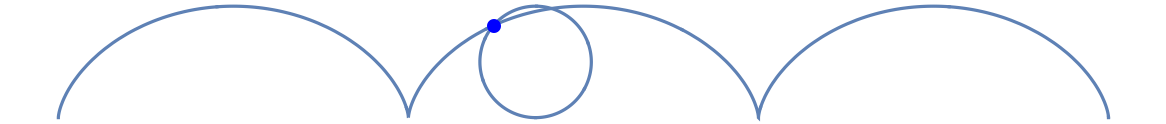
\includegraphics[width=\linewidth]{curvas1}
		  \end{figure}
		\item Basta calcular
		\begin{align*}
			\int_0^{2\pi}|\alpha'(t)|dt&=\int_0^{2\pi}|(1-\cos{t},\sin{t})|dt\\
			&=\int_0^{2\pi}\sqrt{(1-\cos{t})^2+\sin^2{t}}dt\\
			&=\int_0^{2\pi}\sqrt{1-2\cos{t}+\cos^2{t}+\sin^2{t}}dt\\
			&=\int_0^{2\pi}\sqrt{2(1-\cos{t})}dt\\
			&=\sqrt{2}\int_0^{2\pi}\sqrt{1-\cos{t}}dt\\
			&=\ldots=8
		\end{align*}
	\end{enumerate}
\end{proof}

\begin{ejer}[El Folio de Descartes. Ejer 5, Sec 1.3, Do Carmo] Consideremos la curva $\alpha:(-1,+\infty)\to\R^2$ dada por:
\[\alpha(t)=\left(\frac{3at}{1+t^3},\frac{3at^2}{1+t^3}\right)\]
Pruebe que:
\begin{itemize}
	\item Para $t=0$, $\alpha$ es tangente al eje $X$.
	\item Cuando $t\to\infty$, $\alpha \to (0,0)$ y $\alpha'\to(0,0).$
\end{itemize}
\end{ejer}

\begin{proof}[Solución]\leavevmode
	\begin{enumerate}
		\item Claro, pues
		\[\alpha'(t)=\left(\frac{(1+t^3)3a-(3at)(3t^2)}{(1+t^3)^2}, \frac{(1+t^3)6at-(6at^2)(1+3t)}{(1+t^3)^2}\right)\]
		Y si $t=0$, $\alpha'(0)=(3a,0)$.
		
		\item Claro, ya que cuanto $t\to\infty$, las variables en el denominador de ambas entradas "dominan" por tener exponentes de más grandes. Esto sucede tanto para $\alpha$ como para $\alpha'$.
		\begin{figure}[H]
			\centering
			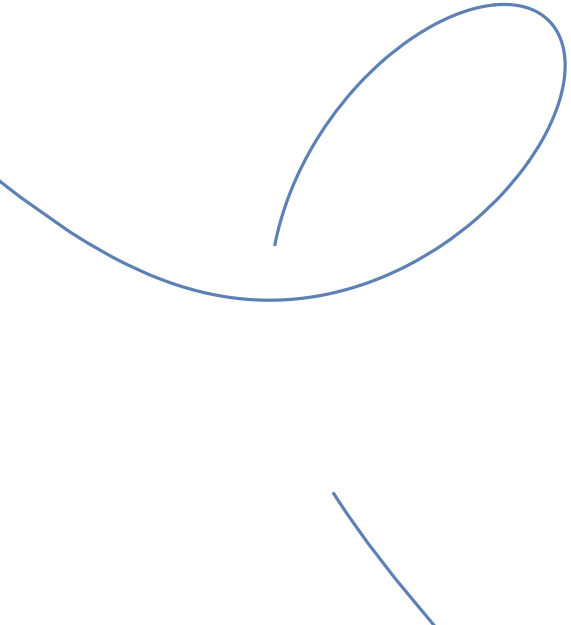
\includegraphics[width=0.3\linewidth]{curvas2}
			\caption*{\textit{Nunca pude completar el dibujo en Mathematica \Smiley}}
		\end{figure}
		\end{enumerate}
\end{proof}

\begin{ejer}[La espiral logarítmica.Ejer 6, Sec 1.3, Do Carmo] Consideremos la curva $\alpha(t)=(ae^{bt}\cos{t}, ae^{bt}\sin{t})$, $t\in\R,a>0,b<0$.
\begin{itemize}
	\item Pruebe que cuando $t\to\infty$, $\alpha(t)$ se aproxima al origen en espirales.
	\item Muestre que $\alpha'(t)\to(0,0)$ cuando $t\to+\infty$ y que
	\[\lim_{t\to+\infty}\int_{t_0}^t|\alpha'(t)| dt\]
	es finito. Es decir, que la longitud de arco de $\alpha$ es finita en el intervalo $(t_0,\infty)$.
\end{itemize}
\end{ejer}

\begin{proof}[Solución]\leavevmode
	\begin{enumerate}
		\item Como $\alpha(t)=(ae^{bt}\cos{t}, ae^{bt}\sin{t})=ae^{bt}(\cos{t},\sin{t})$ y $b$ es una constante negativa (y el coseno  y el seno son funciones acotadas), la norma de esta función se hace pequeña conforme $t\to\infty$.
		\item Calculemos la derivada:
		\begin{align*}
			\alpha'(t)&=a(-e^{bt}\sin{t}+be^{bt}\cos{t},e^{bt}\cos{t}+be^{bt}\sin{t})\\
			&=ae^{bt}(-\sin{t}+b\cos{t},\cos{t}+b\sin{t})
		\end{align*}
		De donde es claro el primer límite. Ahora calculamos la norma de la derivada:
		\begin{align*}
			|\alpha'(t)|&=| ae^{bt}(-\sin{t}+b\cos{t},\cos{t}+b\sin{t})|\\
			&=ae^{bt}\sqrt{(-\sin{t}+b\cos{t})^2+(\cos{t}+b\sin{t})^2}\\
			&=ae^{bt}\sqrt{\sin^2{t}-2b\sin{t}\cos{t}+b^2\cos^2{t}+\cos^2{t}+2b\sin{t}\cos{t}+b^2\sin^2{t}}\\
			&=ae^{bt}\sqrt{1+b^2}
		\end{align*}
		Integramos:
		\begin{align*}
			\int_{t_0}^t|\alpha'(t)| dt&=\int_{t_0}^t ae^{bt}\sqrt{1+b^2}dt\\
			&=a\sqrt{1+b^2}\int_{t_0}^te^{bt}dt\\
			&=a\sqrt{1+b^2}\left[\frac{e^{bt}}{b}\right]_{t_0}^t\\
			&=\frac{a\sqrt{1+b^2}}{b}(e^{bt}-e^{bt_0})
		\end{align*}
		que tiende a una cantidad finita cuando $t\to\infty$ ya que $b$ es negativo.
	\end{enumerate}
\end{proof}

\section{Evoluta}
En el ejercicio 7* de la sección 1.5 del Do Carmo y en el ejercicio 3 de la sección 2.30 tenemos la siguiente definición:
\begin{defn}
	Consideremos una curva $\alpha:I\to\R^2$ regular, plana ($\tau\equiv0$) no necesariamente parametrizada por 		longitud de arco, cuya curvatura está dada por
	\[\frac{d\mathbf{T}}{dt}=k\mathbf{N}\]
	donde $\mathbf{T}$ es el vector tangente unitario y $\mathbf{N}$ el normal unitario al tiempo $s$. Suponiendo que $k(t)\neq0$ 		para $t\in I$, definimos la \textbf{evoluta} de $\alpha$ como
	\[\beta(t)=\alpha(t)+\frac{1}{k(t)}\mathbf{N}(t),\qquad t\in I\]
	Se trata del lugar geométrico de los centros de los círculos osculadores en cada momento en el tiempo. Los círculos osculadores son aquellos que tienen la misma tangente en cada punto de la curva, y también la misma curvatura. Es el círculo que mejor aproxima a la curva.
\end{defn}

\begin{ejer}[La evoluta de la parábola] Calcule la evulta de la parábola unitaria $(t,t^2)$. ¿Esta curva tiene singularidades?
\end{ejer}
\begin{proof}
	Comencemos por ver quién es el vector tangente:
	\[\mathbf{T}=\frac{d}{dt}(t,t^2)=(1,2t)\]
	Luego, el tangente unitario está dado por
	\[\frac{\mathbf{T}}{\Vert \mathbf{T}\Vert}=\frac{1}{\sqrt{1+4t^2}}(1,2t)\]
	Y el normal unitario es ese vector rotado 90º grados en dirección antihoraria:
	\[\mathbf{N}=\frac{1}{\sqrt{1+4t^2}}(-2t,1)\]
	Como no sabemos cuál es una parametrización por longitud de arco, usamos la fórmula en el Ejercicio 12(d), Sección 1.5 Do Carmo, que aplica para curvas planas de la forma $(x(t),y(t))$:
	\[k(t)=\frac{x'y''-x''y'}{\left((x')^2+(y')^2\right)^{3/2}}\]
	En nuestro caso,
	\[x'=1\qquad x''=0\qquad y'=2t\qquad y''=2\]
	así que
	\[k(t)=\frac{2}{(1+(2t)^2)^{3/2}}=\frac{2}{(1+4t^2)^{3/2}}\]
	O sea que la evoluta es:
	\begin{align*}
		\beta(t)&=(t,t^2)+\frac{(1+4t^2)^{3/2}}{2}\frac{1}{\sqrt{1+4t^2}}(-2t,1)\\
		&=(t,t^2)+\frac{1+4t^2}{2}(-2t,1)
	\end{align*}
	Para saber si la curva tiene singularidades, derivamos e igualamos a cero. Encontramos que en $t=0$ la curva tiene una singuladgridad:
	\begin{figure}[H]
		\centering
		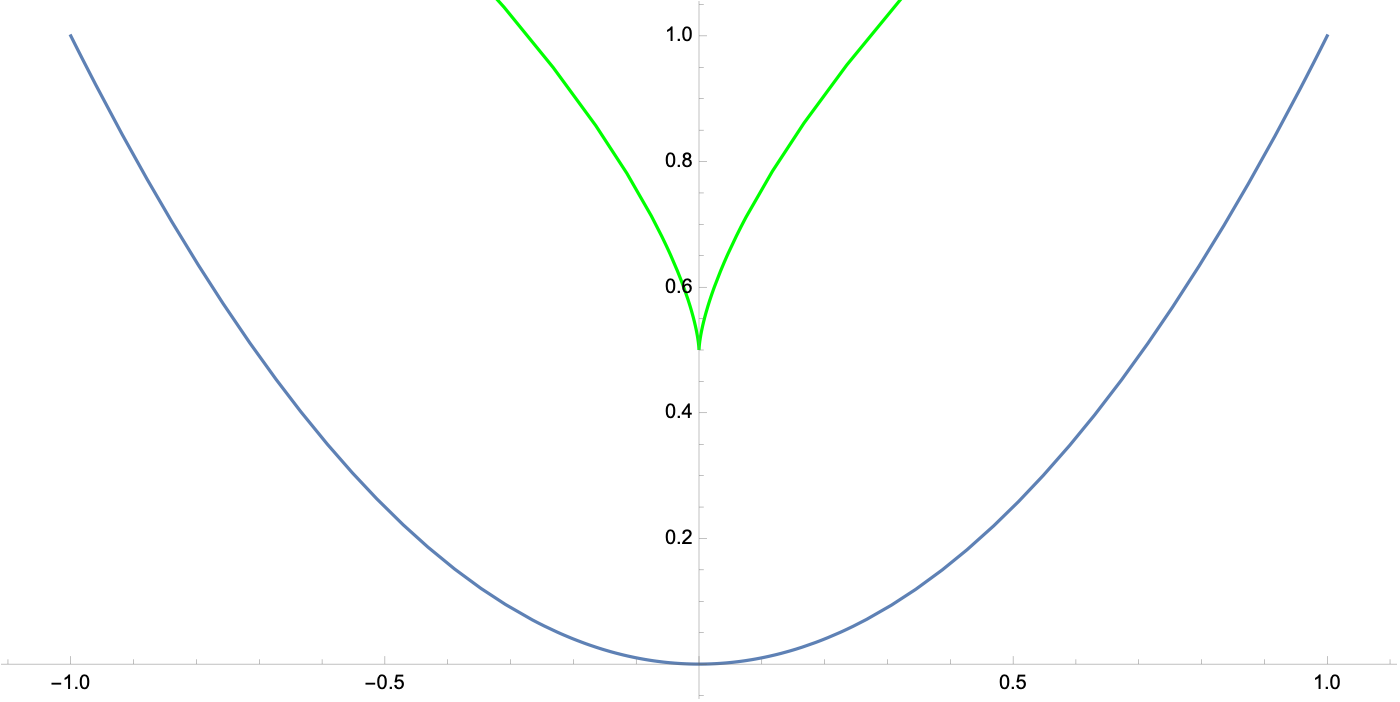
\includegraphics[width=0.7\linewidth]{curvas3}
	\end{figure}
\end{proof}
\begin{obs}
	La circunferencia de radio R tiene una arametrización por longitud de arco dada por:
	\begin{align*}
		\alpha:[0,&2\pi]\to \R^2\\
		t&\mapsto (R\cos{\frac{t}{R},R\sin{\frac{t}{R}}})
	\end{align*}
	Ya que 
	\[\alpha'(t)=(-\sin{\frac{t}{R}},\cos{\frac{t}{R}})\]
	es de norma 1.
\end{obs}
\begin{ejem}[La evoluta de la elipse]
	La parametrización por longitud de arco no resulta tan sencilla para el caso de la elipse, pero sí es posible encontrar una expresión para la evoluta usando otro método para encontrar la curvatura **(Falta).**
	La curva resulta ser así:
	\begin{figure}[H]
		\centering
		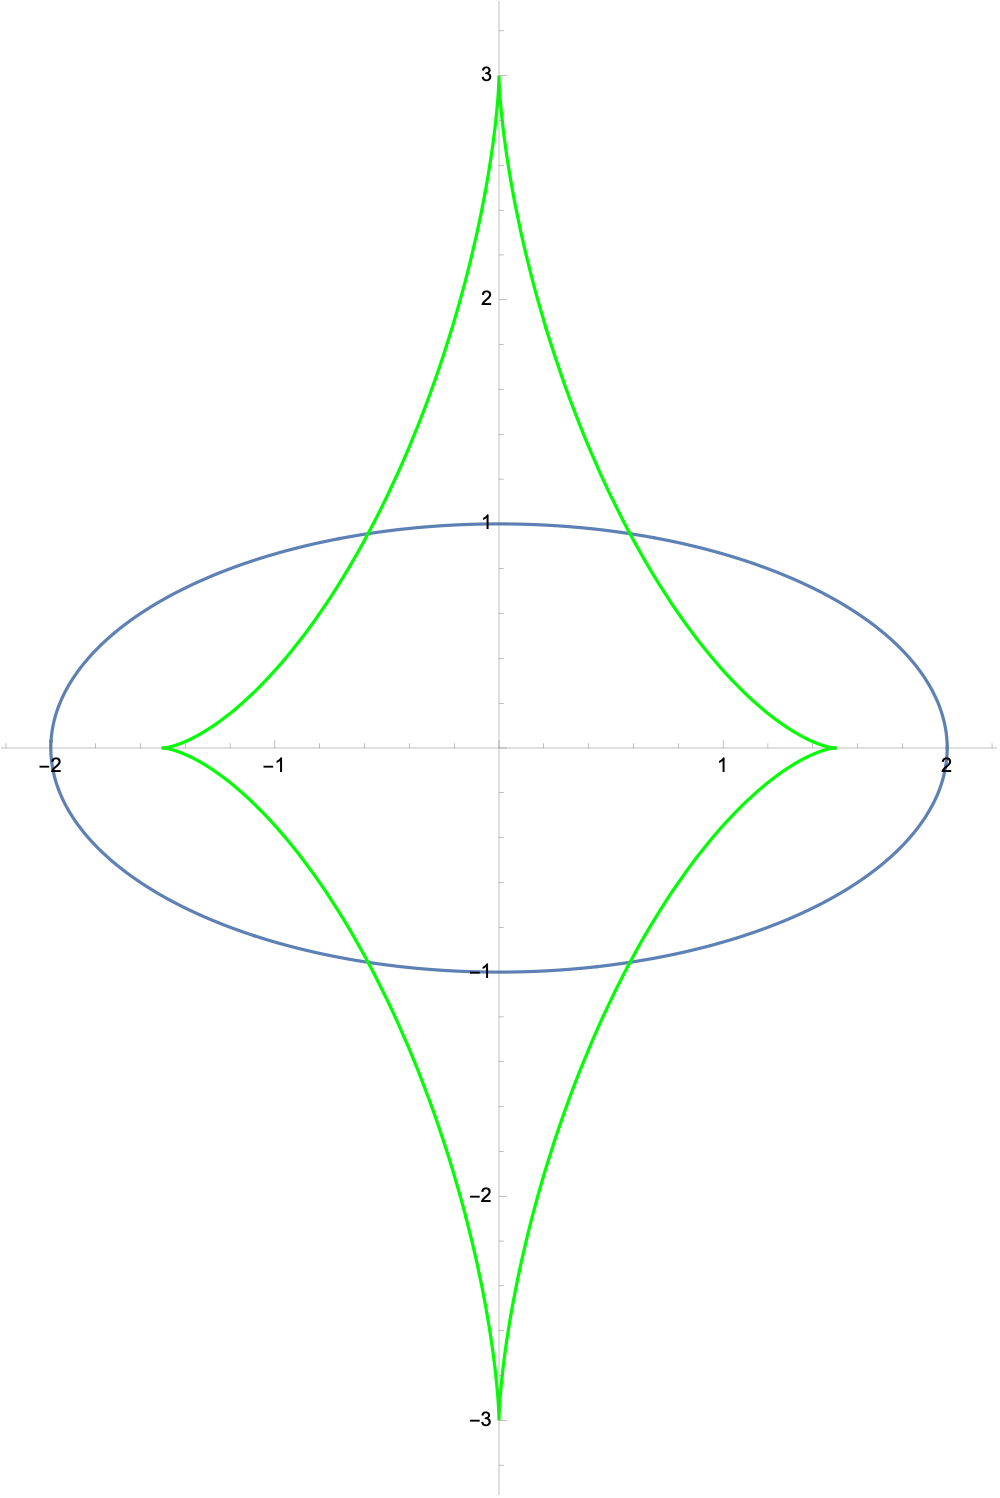
\includegraphics[width=0.7\linewidth]{curvas4}
	\end{figure}
\end{ejem}
\begin{pregunta}
	¿Cómo detectamos las singularidades en la evoluta?
\end{pregunta}
Visualmente, notamos que las singularidades en la evoluta corresponden con los puntos máximos y mínimos de la curvatura de la elipse. De hecho, esto se puede formalizar en el siguiente ejercicio.
\begin{defn}
	El radio de curvatura $\rho$ es el radio del círculo osculador, ie. $\rho=\frac{1}{\kappa}$.
\end{defn}
\begin{ejer}[Ejercicio 2.26(3), Bruce\&Giblin]
	Consideremos una curva plana $\alpha:I\to\R^2$ parametrizada por longitud de arco y tal que $\kappa(t)$ nunca es cero.
	\begin{enumerate}
		\item Muestre que la evoluta es regular salvo por los puntos donde $k'(t)=0$. Estos puntos se llaman "vértices" de la curva.
		\item Supongamos que $k'(t)<0$ en $I$. Muestre que la longitud de arco de la evoluta de $t_0$ a $t_1$, para $t_1>t_0\in I$, es $\rho(t_1)-\rho(t_0)$.
		\item Nuevamente suponiendo que $\kappa'(t)<0$, muestre que el tangente unitario y el normal a $\varepsilon$ satisfacen que
		\[\mathbf{T}_\varepsilon=\mathbf{N},\qquad\mathbf{N}_\varepsilon=-\mathbf{T},\qquad \kappa_\varepsilon=-\kappa^3/\kappa'\]
 		de forma que la evoluta no tiene inflexiones. **Falta el de la curvatura.**
 		\item Una vez más tomemos $\kappa'(t)<0$. Supongamos que amarramos una cuerda en algún punto de la curva $\alpha(t_0)$. Amarremos la cuerda primero al punto correspondiente en la evoluta, $\varepsilon(t_0)$, y luego recorramos sobre la evoluta hasta llegar a algún punto $\varepsilon(t)$. Pruebe que el tamaño de la cuerda es $\Vert \varepsilon(t)-\alpha(t)\Vert$.
	\end{enumerate}
\end{ejer}
\begin{obs}[Comentarios sobre el inciso 3]
	Las inflexiones son puntos donde la curvatura cambia de signo. Para gráficas de funciones, es cuando la curva pasa de ser cóncava a convexa. Por otro lado, las inflexiones son puntos de contacto de orden $\geq3$, que se mide viendo cuántas derivadas se hacen cero en el punto.
\end{obs}
\begin{proof}[Solución]
	\begin{enumerate}
		\item Derivando la ecuación general de la evoluta,
		\[\varepsilon(t)=\alpha(t)+\frac{1}{\kappa(t)}\mathbf{N}(t),\qquad t\in I\]
		obtenemos
		\begin{align*}
			\varepsilon'(t)&=\alpha'(t)+\frac{k(t)\mathbf{N}'(t)-k'(t)\mathbf{N}(t)}{k(t)^2}\\
			&=\alpha'(t)+\frac{\mathbf{N}'(t)}{k(t)}-\frac{k'(t)}{k(t)^2}\mathbf{N}(t)\\
		\end{align*}
		Ahora como la parametrización es por longitud de arco, podemos aplicar Frenet-Serret para obtener
		\begin{align*}
			\varepsilon'(t)&=\mathbf{T}(t)+\frac{\mathbf{N}'(t)}{k(t)}-\frac{k'(t)}{k(t)^2}\mathbf{N}(t)\\\\
			&=\mathbf{T}(t)+\frac{-k(t)\mathbf{T}(t)+\tau(t)\mathbf{B}(t)}{k(t)}-\frac{k'(t)}{k(t)^2}\mathbf{N}(t)\\
			&=-\frac{k'(t)}{k(t)^2}\mathbf{N}(t)
		\end{align*}
		ya que la curva es plana.
		\item Basta calcular la integral
		\begin{align*}
			\int_{t_0}^{t_1}\Vert\varepsilon'(t)\Vert dt&=\int_{t_0}^{t_1}\Big\Vert-\frac{\kappa'(t)}{\kappa(t)^2}\mathbf{N}(t)\Big\Vert dt\\
			&=\int_{t_0}^{t_1}\frac{\kappa'(t)}{\kappa(t)^2} dt\\
			&=\Big[\frac{1}{\kappa(t)}\Big]_{t_0}^{t_1}\\
			&=\rho(t_1)-\rho(t_0)
		\end{align*}
		\item Notemos que aunque la curva $\alpha$ está parametrizada por longitud de arco, esto no necesariamente es cierto para su evoluta. Calculemos el vector tangente unitario de la evoluta:
		\[\mathbf{T}_\varepsilon=-\frac{\frac{\kappa'(t)}{\kappa(t)^2}\mathbf{N}(t)}{\Vert\varepsilon'(t)\Vert}\]
		donde, como $\kappa'(t)<0$,
		\[\Vert\varepsilon'(t)\Vert=\Big|-\frac{\kappa'(t)}{\kappa(t)^2}\Big|=-\frac{\kappa'(t)}{\kappa(t)^2}\]
		Ahora, el vector normal de la evoluta es rotar el tangente en dirección antihoraria, lo que naturalmente nos devuelve $-\mathbf{T}$.
		Por último, si intentamos calcular la curvatura usando la fórmula para curvas planas
		\begin{align*}
			\kappa(t)&=\frac{\det{(\varepsilon'(t),\varepsilon''(t))}}{\Vert \varepsilon'(t)\Vert^3}\\
		\end{align*}
		tendríamos que calcular la segunda derivada de $\varepsilon$ para ver si algo se simplifica:
		\begin{align*}
			\varepsilon''(t)&=-\frac{d}{dt}\frac{\kappa'(t)}{\kappa(t)^2}\mathbf{N}(t)\\
			&=-\Big(\frac{\kappa'(t)}{\kappa(t)^2}\mathbf{N}'(t)+\frac{d}{dt}\frac{\kappa'(t)}{\kappa(t)^2}\mathbf{N}(t)\Big)\\
			&=-\Big(-\frac{\kappa'(t)}{\kappa(t)^2}\kappa(t)\mathbf{T}(t)+\frac{\kappa(t)^2\kappa''(t)-2\kappa'(t)^2\kappa(t)}{\kappa(t)^4}\mathbf{N}(t)\Big)\\
			&=\frac{\kappa'(t)}{\kappa(t)}\mathbf{T}(t)-\frac{\kappa(t)\kappa''(t)-2\kappa'(t)^2}{\kappa(t)^3}\mathbf{N}(t)\\
		\end{align*}
		Ahora para simplificar nuestro camino recordemos que queremos llegar a que $\kappa_\varepsilon=-\kappa^3/\kappa'$, y el denominador es
		\[-\frac{\kappa'(t)^3}{\kappa(t)^6}\]
		Este camino no funciona...
		
		Otra idea es: si tuviéramos una parametrización por longitud de arco de $\varepsilon$, tendríamos Frenet-Serret, es decir
		\[\frac{d}{dt}\mathbf{T}_\varepsilon(t)=\kappa_\epsilon(t)\mathbf{N}_\varepsilon(t)\]
		donde
		\[\frac{d}{dt}\mathbf{T}_\varepsilon(t)=\frac{d}{dt}\mathbf{N}(t)=-\kappa(t)\mathbf{T}(t)\]
		Y como además $\mathbf{N}_\varepsilon=-\mathbf{T}$, llegaríamos a la contradicción de que $\kappa_\varepsilon=\kappa$. **Hasta aquí por ahora...**
		\item Queremos demostrar que
		\[\Vert\alpha(t)-\varepsilon(t)\Vert=\Vert\alpha(t_0)-\varepsilon(t_0)\Vert+\int_{t_0}^t\Vert\varepsilon'(t)\Vert dt\]
		Y ya sabemos que la integral vale $\rho(t)-\rho(t_0)$. Ahora la distancia de un punto en la curva a su punto correspondiente en la evoluta es:
		\begin{align*}
			\Vert\alpha(t)-\varepsilon(t)\Vert&=\Big\Vert\alpha(t)-\alpha(t)-\frac{1}{\kappa(t)}\mathbf{N}(t)\Big\Vert\\
			&=\Big\Vert-\frac{1}{\kappa(t)}\mathbf{N}(t)\Big\Vert\\
			&=\Big|\frac{1}{\kappa(t)}\Big|\\
			&=|\rho(t)|
		\end{align*}
		Así, lo que queremos ver es simplemente que 
		\begin{align*}
			|\rho(t)|&=|\rho(t_0)|+\rho(t)-\rho(t_0)\\
			\iff |\rho(t)|-\rho(t)&=|\rho(t_0)|-\rho(t_0)\\
		\end{align*}
		   que se cumple en cualquier caso:
		\begin{itemize}
			\item Si $\rho(t)>0$ y $\rho(t_0)>0$ es trivial.
			\item El caso $\rho(t)>0$ y $\rho(t_0)<0$ no es posible porque eso implica que $\kappa(t)=0$, que no es posible por hipótesis. Lo análogo sucede si $\rho(t)<0$ y $\rho(t_0)>0$
			\item Si $\rho(t)<0$ y $\rho(t_0)<0$, tenemos que $\rho(t)=\rho(t_0)$, pero esto tampoco es posible porque $\kappa'<0$.
			\begin{figure}
				\centering
				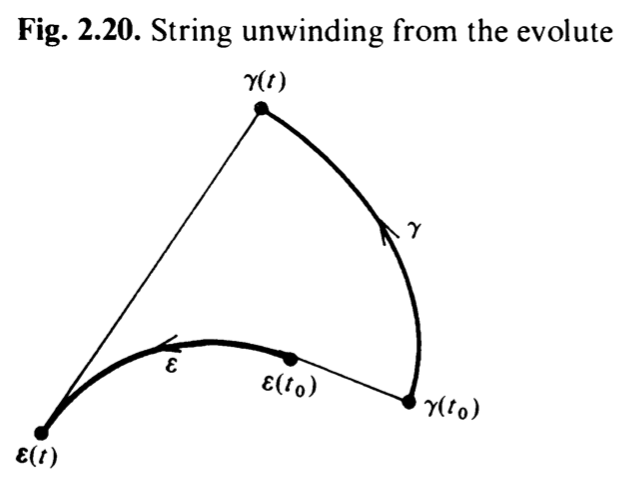
\includegraphics[width=0.4\linewidth]{curvas5}
			\end{figure}
		\end{itemize}
	\end{enumerate}
\end{proof}
\begin{ejem}[La evoluta de la gráfica del coseno]
	Para una curva con puntos de inflexión, la evoluta tiene puntos al infinito:
	\begin{figure}[H]
		\centering
		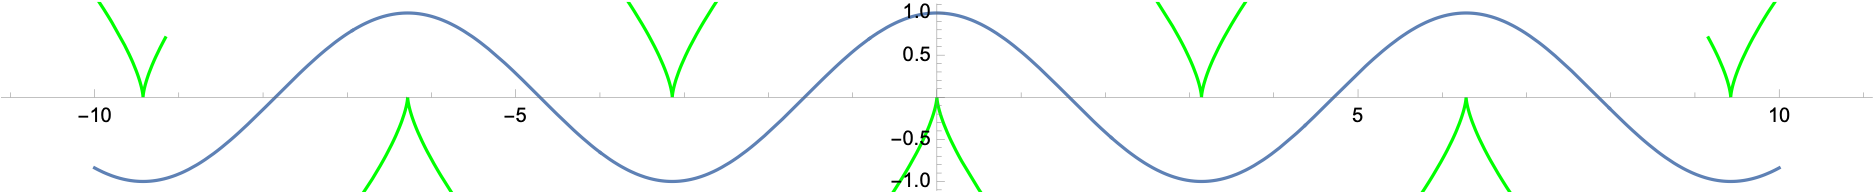
\includegraphics[width=0.8\linewidth]{curvas6}
	\end{figure}
	Si tratamos de ver la imagen completa:
	\begin{figure}[H]
		\centering
		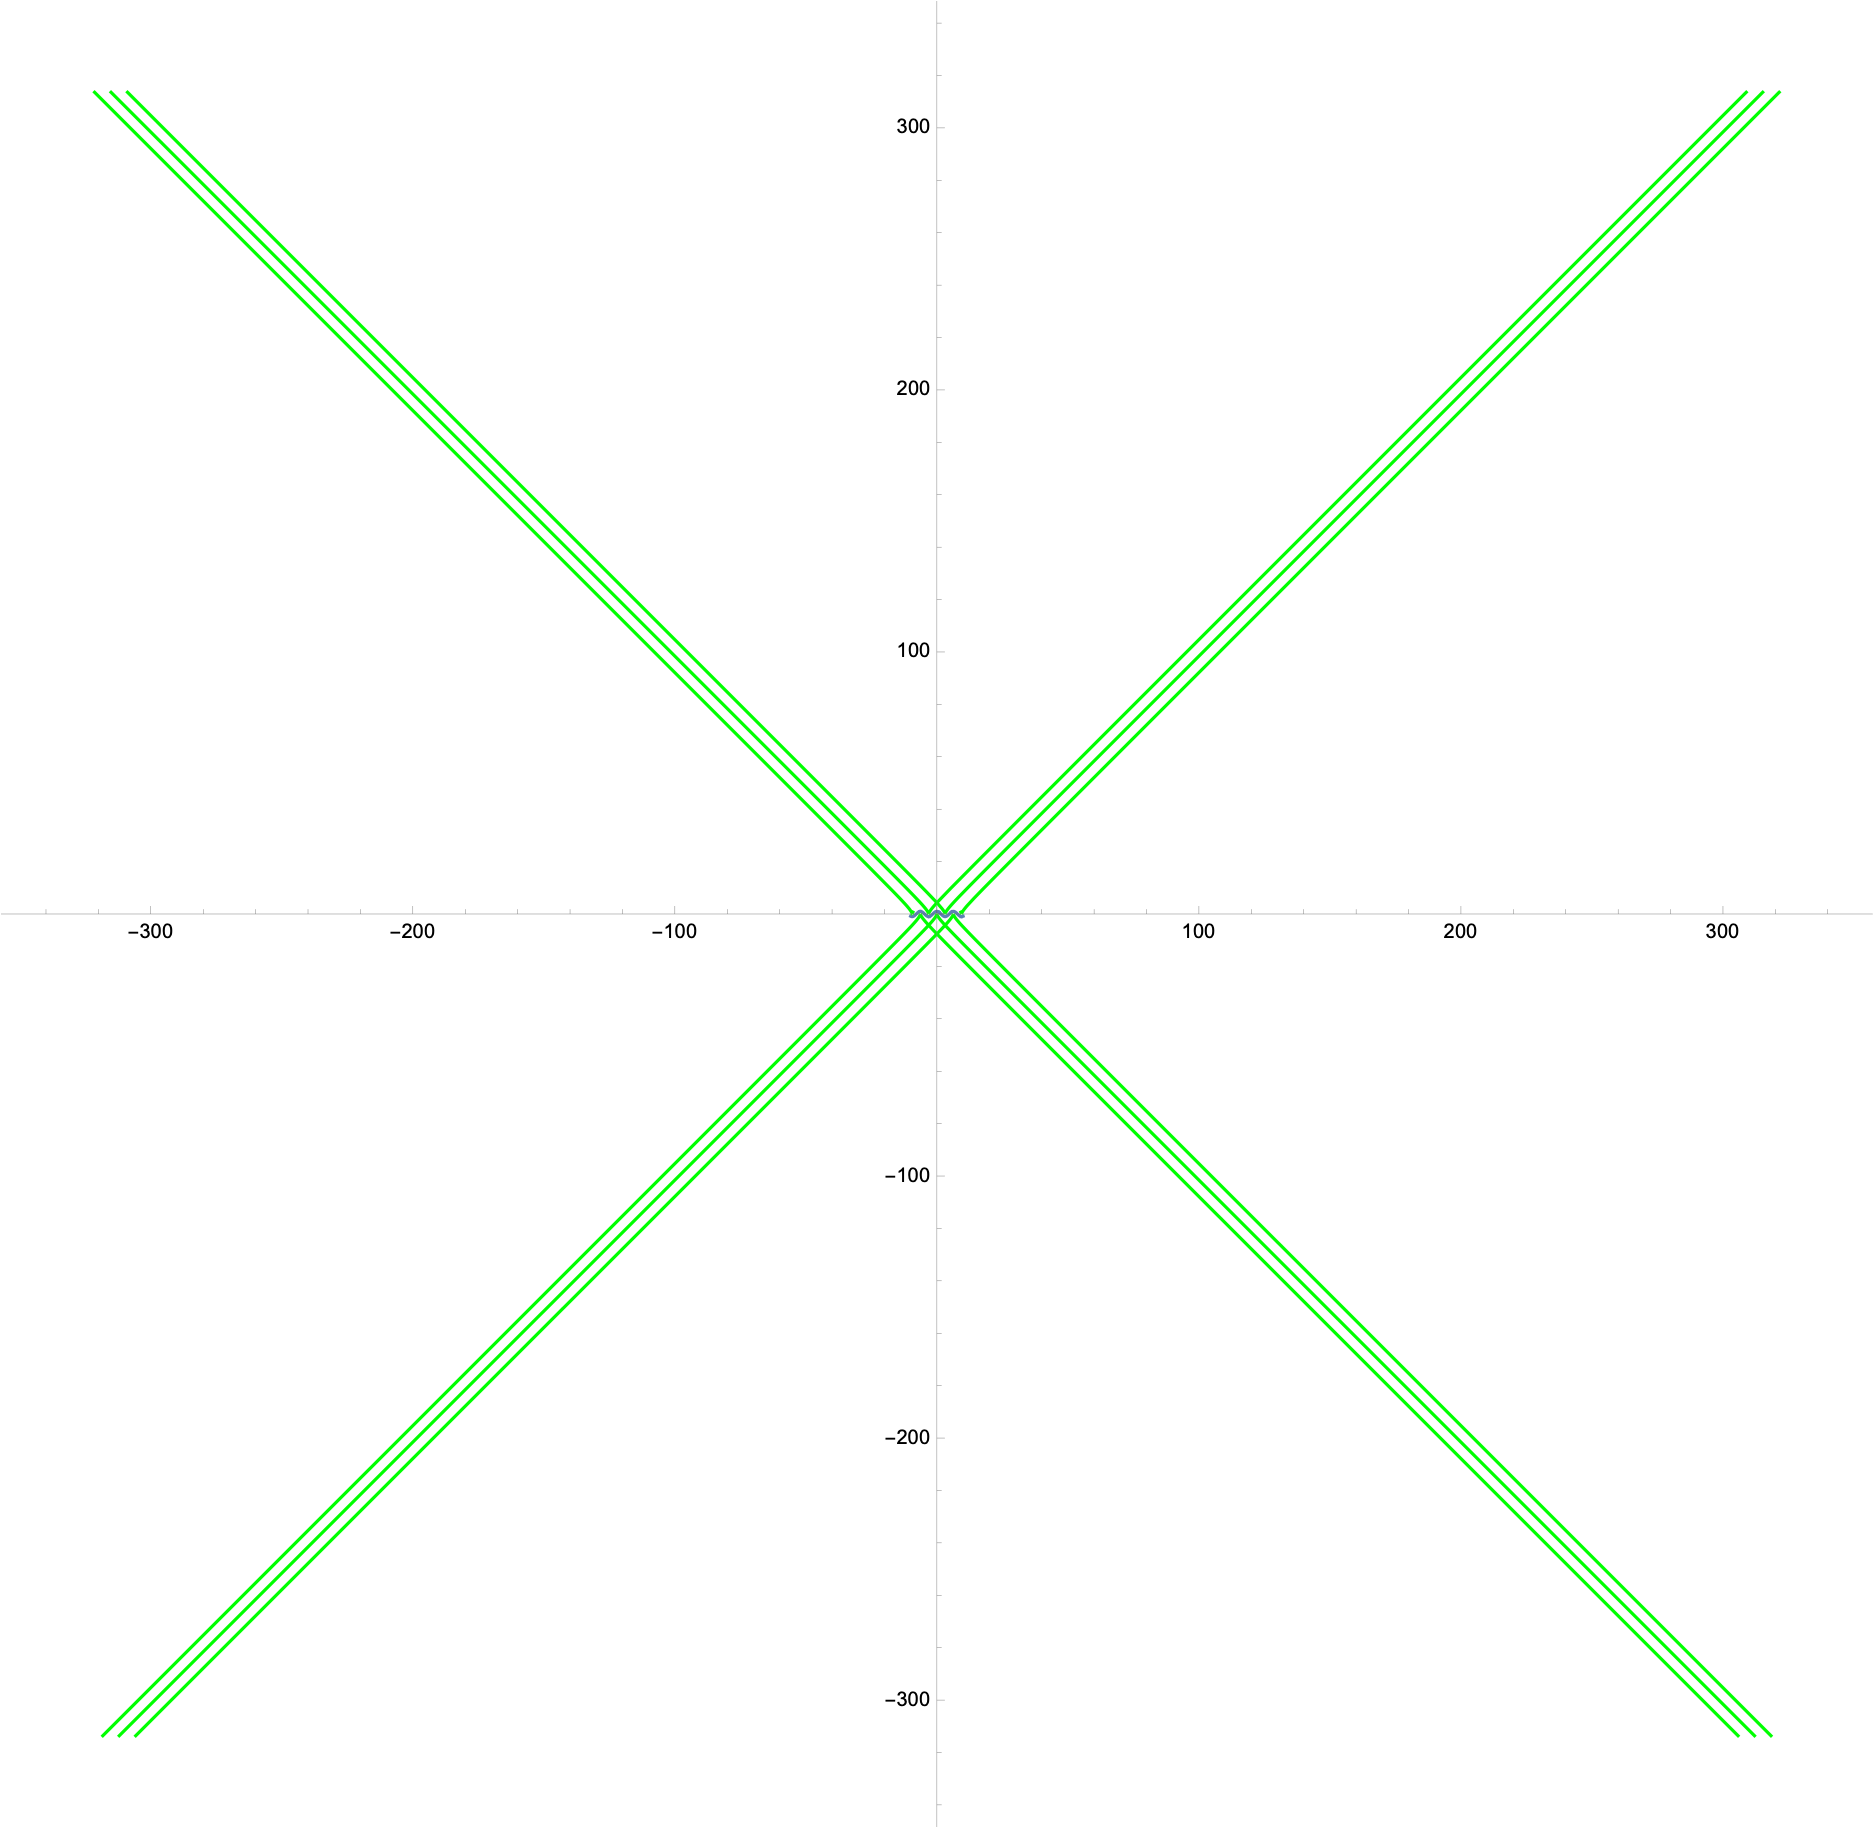
\includegraphics[width=0.9\linewidth]{curvas7}
	\end{figure}
\end{ejem}
\section{Podaria}
\begin{ejer}[2.26(1), Bruce\&Giblin]
	La curva podaria es el lugar geométrico de las proyecciones ortogonales del origen en la recta tangente. Para encontrar una parametrización, observemos el siguiente diagrama:
	\begin{figure}[H]
		\centering
		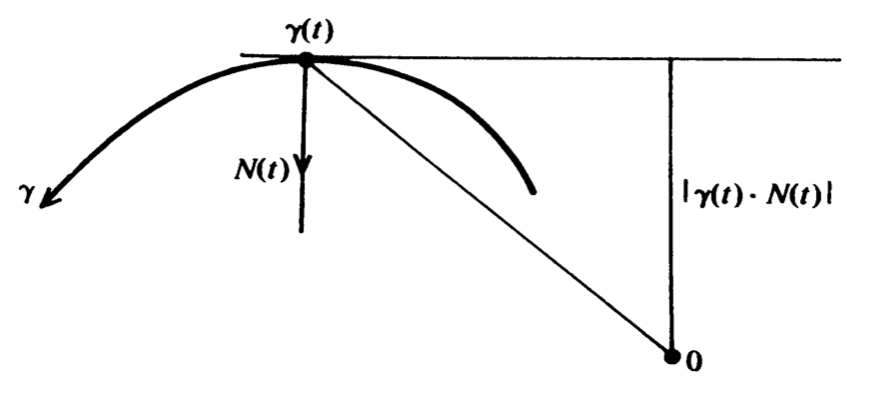
\includegraphics[width=0.7\linewidth]{curvas8}
	\end{figure}
	Al ser el punto que buscamos ortogonal a la recta tangente, debe ser un múltiplo del vector normal. Para encontrar su magnitud, observamos en el diagrama que el ángulo entre $\gamma (t)$ y $\mathbf{N}(t)$ es adyacente al vector que buscamos. Usando trigonometría clásica, el coseno de este ángulo por el tamaño de la hipotenusa del triángulo rectángulo nos da la magnitud buscada, es decir:
	\[|\text{lado adyacente}|=|\gamma(t)|\cos{\theta}=\gamma(t)\cdot\mathbf{N}(t)\]
	Así, la curva podaria simplemente es
	\[\delta(t)=\big(\gamma(t)\cdot\mathbf{N}(t)\big)\mathbf{N}(t)\]
	
	Que, por una cuenta sencilla suponiendo una parametrización por longitud de arco tiene derivada
	\[\delta'=-\kappa\Big((\gamma\cdot\mathbf{T})\mathbf{N}+(\gamma\cdot\mathbf{N})\mathbf{T}\Big)\]
	De forma que las singularidades son cuando la curva es plana o cuando pasa por el origen. *Observación. Bruce\&Giblin escriben que "**El segundo factor** de $\delta'$ se hace cero si y sólo si la curva pasa por el origen ".* En el libro también se menciona que si la curva no pasa por el origen, $\delta$ es regular salvo en los puntos de inflexión.
\end{ejer}
\begin{ejem}[La podaria de una circunferencia con centro en (1,0)]
	Resulta que cuando calculamos la podaria desde un punto en la circunferencia obtenemos la cardioide. Para esto, mejor calculamos la podaria de una circunferencia trasladada.
	\begin{figure}[H]
		\centering
		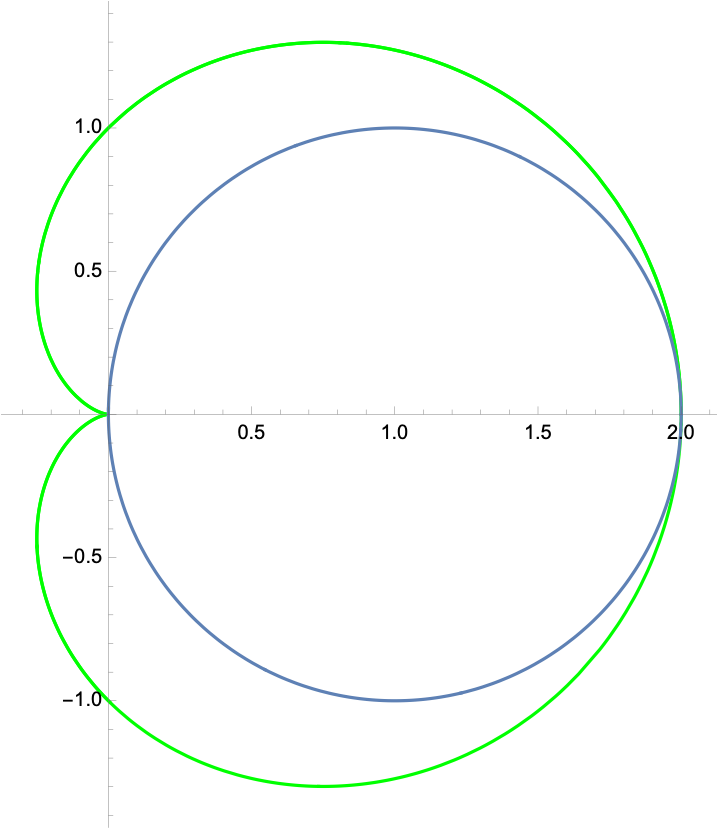
\includegraphics[width=0.7\linewidth]{curvas9}
	\end{figure}
\end{ejem}
\begin{pregunta}
	¿Qué otros ejemplos padres hay de curvas podarias?
\end{pregunta}

\section{Paralela}
\begin{ejer}[2.26(2), Bruce\&Giblin]
	Dada una curva plana parametrizada por longitud de arco $\alpha$, y un número real positivo $d$, las curvas del estilo
	\[\delta(t)=\alpha(t)+d\mathbf{N}(t)\]
	son llamadas curvas paralelas a $\alpha$. Aquí hay una familia de curvas paralelas a la parábola unitaria (rosa) para valores de $d$ menores que 1.
	\begin{figure}[H]
		\centering
		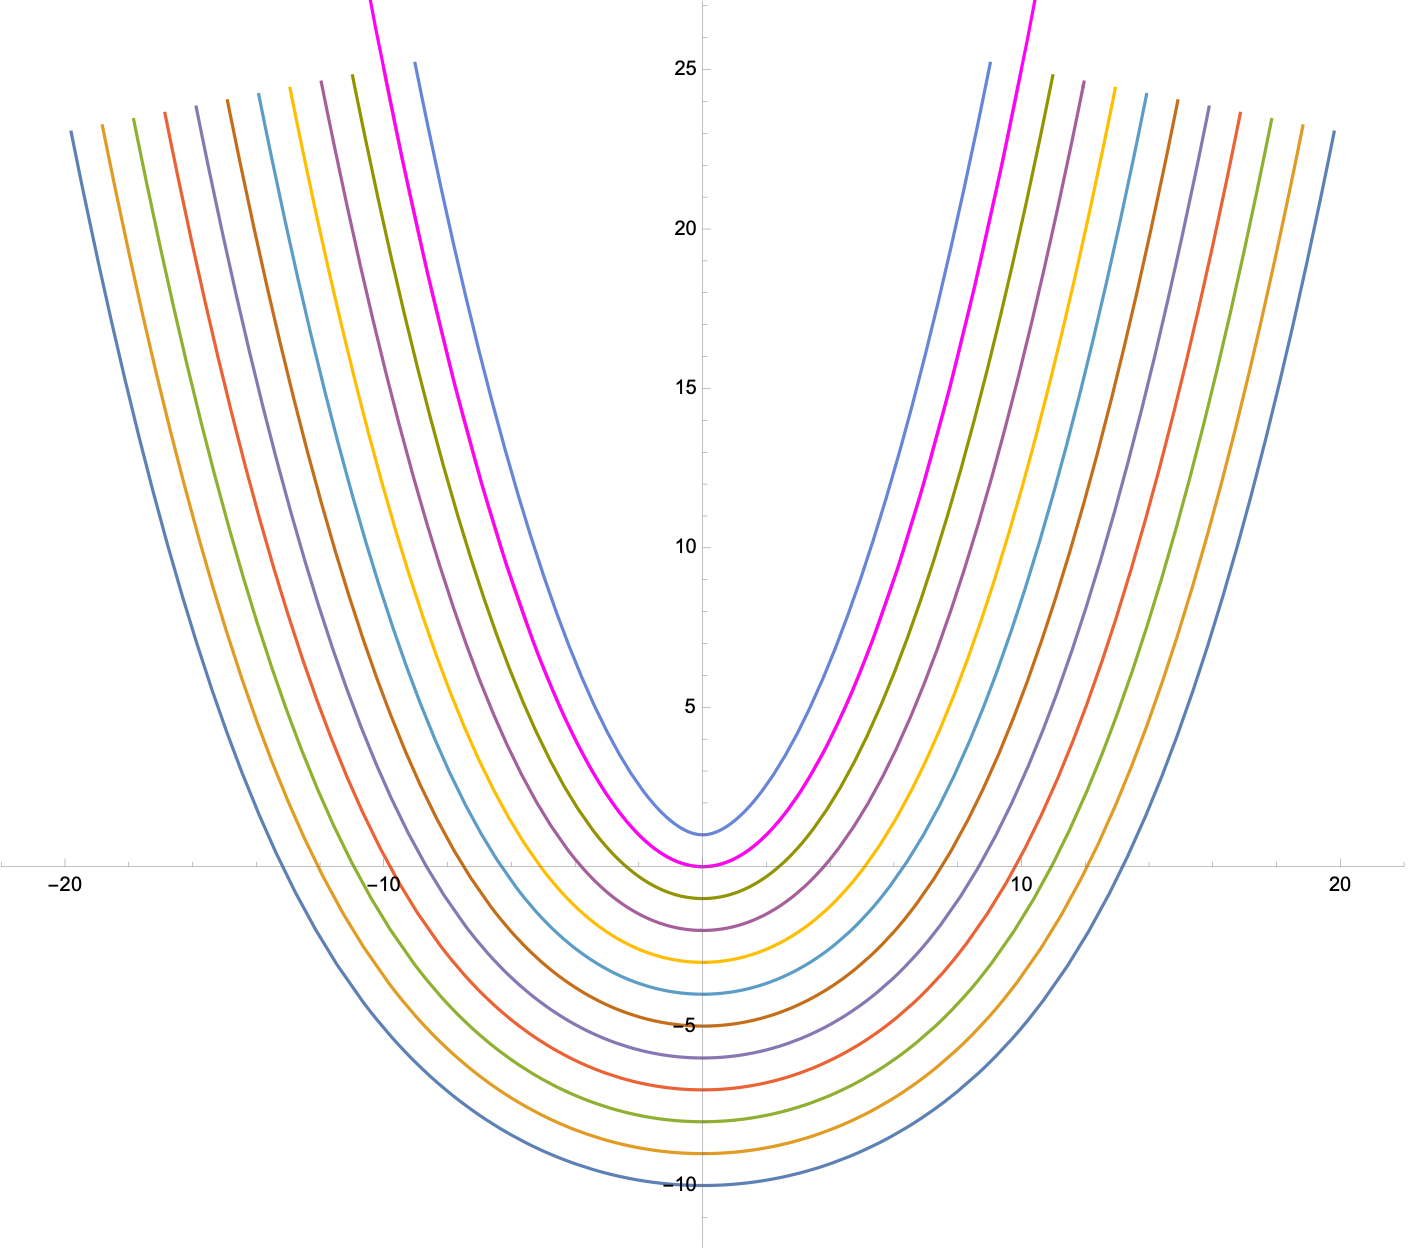
\includegraphics[width=0.7\linewidth]{curvas10}
	\end{figure}
	En general, una curva paralela es regular salvo en los puntos donde $\kappa(t)\neq0$ y $d=1/\kappa(t)$. Y de hecho, los puntos singulares de las curvas paralelas están precisamente en los centros de curvatura de la curva original **(Falta)**. Si calculamos las curvas paralelas a la parábola para valores de $d$ entre -10 y 40 obtenemos la siguiente figura:
	\begin{figure}[H]
		\centering
		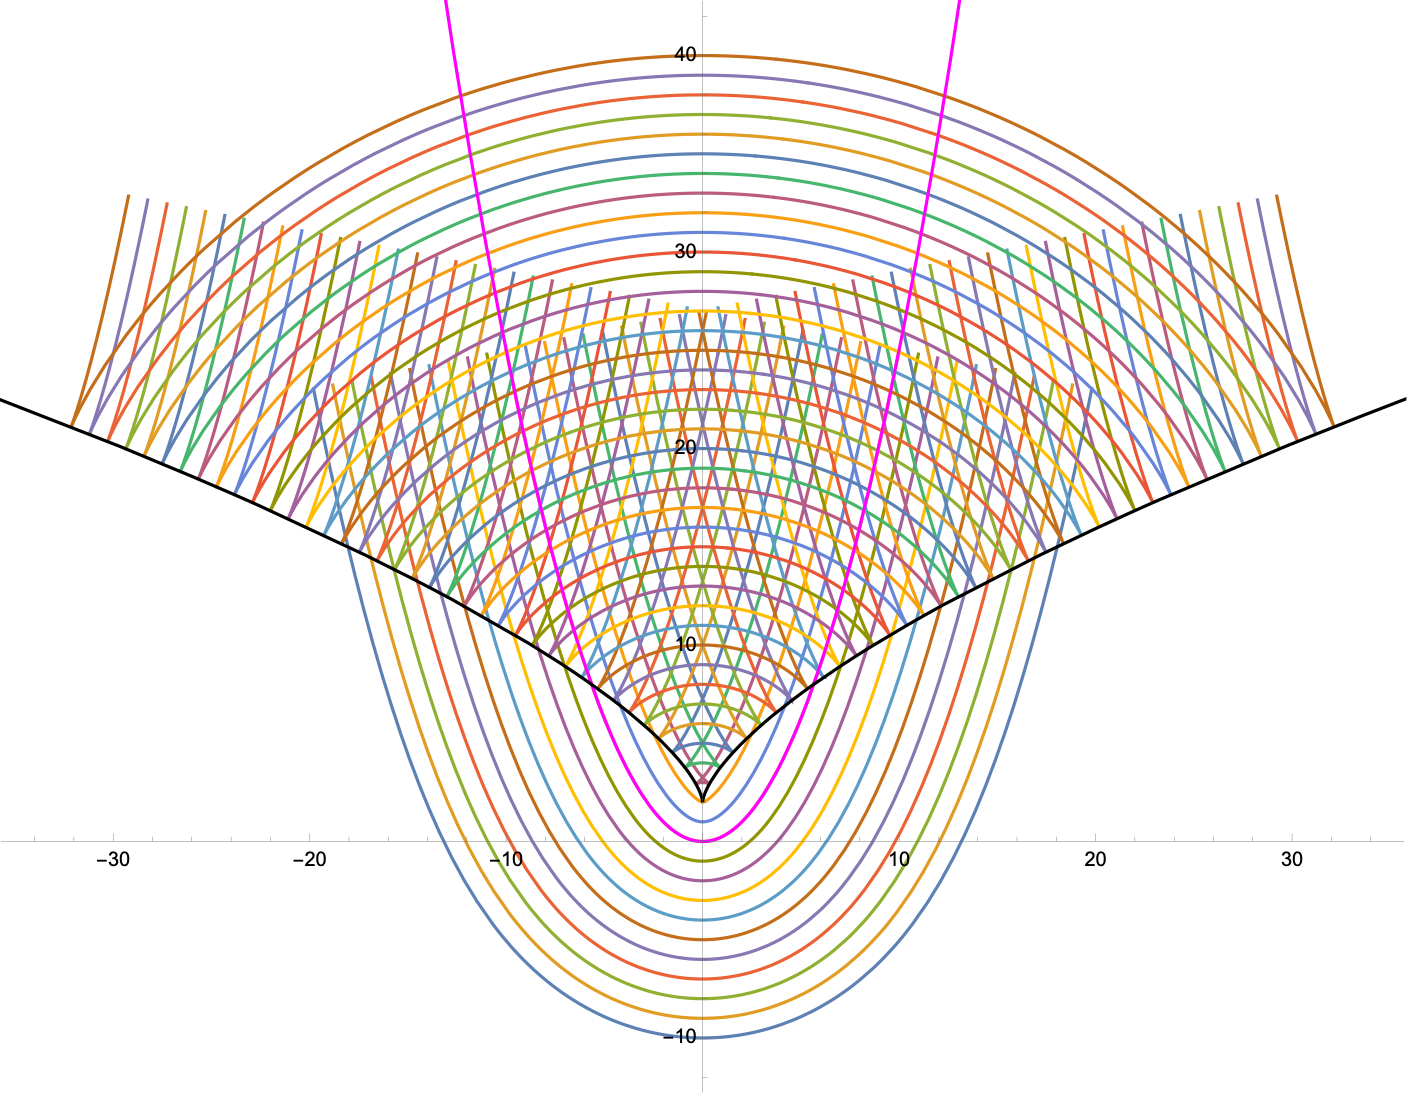
\includegraphics[width=0.7\linewidth]{curvas11}
	\end{figure}
	Aquí vemos que las singularidades de las curvas paralelas a la parábola para valores de $d$ grandes están en la evoluta, que es la curva en color negro y estudiamos anteriormente.
\end{ejer}

\chapter{Superficies}
\section{Primeros ejemplos}
\begin{obs}[Sobre la definición]
	En la definición de superficie regular pedimos que la diferencial de la parametrización local sea inyectiva. Esto es equivalente a que las columnas de la matriz sean linealmente independientes y por eso podemos definir el plano tangente. (El rango de una matriz es la cantidad de columnas linealmente indepientes). Comparemos esto con la condición de suprayectividad: es equivalente a que los renglones sean linealmente independientes.
\end{obs}
\begin{ejem}[La esfera]
	Usando seis parametrizaciones locales de la forma
	\[\mathbf{x_1}=\big(x,y,\sqrt{1-(x^2+y^2)}\big)\qquad,\qquad(x,y)\in\{(x,y)\in\R^2|x^2+y^2\leq1\}\]
	Hay que comprobar las tres propiedades de la definición de do Carmo para superficies regulares. La inversa de la parametrización es la proyección. Las demás $\mathbf{x_i}$ se dan análogamente.
	
	Otra parametrización útil está dada en coordenadas esféricas:
	\[\mathbf{x}(\theta,\varphi)=(\sin{\theta}\cos\varphi,\sin\theta\sin\varphi,\sin\theta)\]
\end{ejem}

\begin{ejem}[El toro como  superficie regular. Do Carmo, Sección 2.2, ejemplo 4, ]
	Sea $S^1$ el círculo de radio $r$ en el plano $yz$ con centro en el punto $(0,a,0)$. Es decir, $S^1=\{(x,y,z)\in\R^3:(y-a)^2+z^2=r^2\}$. Resulta que al rotar este círculo alrededor del eje $z$ obtenemos el conjunto
	\[T=\{(x,y,z)\in\R^3:(\sqrt{x^2+y^2}-a)^2+z^2=r^2\}\]
	Ahora consideremos la función
	\[f(x,y,z)=(\sqrt{x^2+y^2}-a)^2+z^2\]
	Entonces, $T=f^{-1}(r^2)$. Para ver que el toro es una superficie regular, es suficiente demostrar $f$ es diferenciable y $r^2$ es un valor regular de $f$. Derivemos:
	\[\frac{\partial f}{\partial z}=2z\qquad\qquad\frac{\partial f}{\partial y}=\frac{2y(\sqrt{x^2+y^2}-a)}{\sqrt{x^2+y^2}}\qquad\qquad\frac{\partial f}{\partial x}=\frac{2x(\sqrt{x^2+y^2}-a)}{\sqrt{x^2+y^2}}\]
	Así que siempre $(x,y)\neq(0,0)$ tenemos que $f$ es diferenciable, y entonces es suficiente definir el dominio de $f$ como $\R^3-\text{eje }z$. La única forma de que esta derivada como transformación lineal no sea suprayectiva es que sea idénticamente cero, lo que nunca sucede en nuestro dominio.
\end{ejem}

\begin{ejem}[Parametrización del toro. Do Carmo, Sección 2.2, ejemplo 6]
	Consideremos nuevamente $S^1$, el círclo en el plano $yz$ de radio $r$ y centro $(0,a,0)$. Sus puntos tienen coordenadas $(0,a,0)+(0,r\cos{\varphi},r\sin{\varphi})=(0,a+r\cos{\varphi},r\sin{\varphi})$. Ahora tomemos la rotación respecto al eje $z$:
	\[R_z(\theta)=\begin{pmatrix}-\sin\theta&\cos\theta&0\\ \cos\theta&\sin\theta&0\\0&0&1\end{pmatrix}\]
	Aplicando la rotación obtenemos los puntos
	\[\begin{pmatrix}-\sin\theta&\cos\theta&0\\ \cos\theta&\sin\theta&0\\0&0&1\end{pmatrix}\begin{pmatrix}0\\a+r\cos\varphi\\ r\sin{\varphi}\end{pmatrix}
	=\begin{pmatrix}\cos\theta(a+r\cos{\varphi})\\ \sin\theta(a+r\cos\varphi)\\r\sin\varphi\end{pmatrix}\]
	Dando la vuelta completa alrededor de cada círculo parametrizamos todo el toro, aunque para mostrar que una función $\mathbf{x}(\varphi,\theta)$ dada por la ecuación anterior es una parametrización local, debemos definir el dominio $0<\varphi,\theta<2\pi$. Así, nuestra función es diferenciable en todo punto y además su diferencial es inyectiva.
	
	Para mostrar que además es un homeomorfismo, do Carmo usa el ejercicio anterior y la proposición de que un mapeo local biyectivo sobre una superficie regular que sarisface las condiciones (1) y (3) de la definición, también satisface la (2) (Teorema de la función inversa). Así que sólo falta ver que $\mathbf{x}$ es biyectivo.
	
	Para ver biyectividad según do Carmo:
	\begin{enumerate}
		\item $\sin\varphi=z/r$
		\item Si la norma de la proyección del punto sobre el plano $xy$ es menor que $a$, es decir, cuando el punto está "cerca" del eje $z$, $\sqrt{x^2+y^2}\leq a$, entonces el ángulo $\varphi$ está en el intervalo $[\pi/2,3\pi/2]$.
		\item Lo contrario: $\sqrt{x^2+y^2}\geq a\implies\varphi\in[0,\pi/2]\cup[3\pi/2,2\pi]$
		\item Dado un punto $(x,y,z)$ en el toro y veamos qué valor de $\varphi$ le pega. $x$ y $y$ determinan si estamos en el caso 2 o en el caso 3. Por la observación 1 $\varphi$ está únicamente determinado.
		\item Conociendo $\varphi$, $x$ y $y$ tenemos las igualdades $\cos\theta=x/(a+r\cos\varphi)$ y $\sin\theta=y/(a+r\cos\varphi)$, que en conjunto determinan únicamente a $\theta$.
	\end{enumerate}
\end{ejem}
\begin{pregunta}
		¿Cuántas parametrizaciones locales son necesarias para cubrir todo el toro?
\end{pregunta}
\begin{figure}[H]
	\begin{subfigure}{0.5\textwidth}
			\centering
		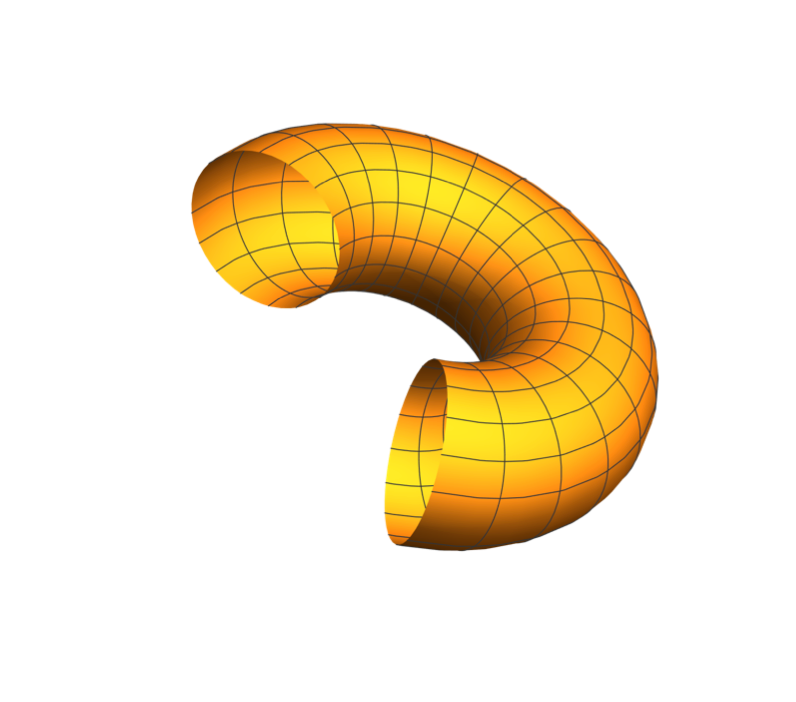
\includegraphics[width=\linewidth]{sup1}
	\end{subfigure}
	\begin{subfigure}{0.5\textwidth}
		\centering
		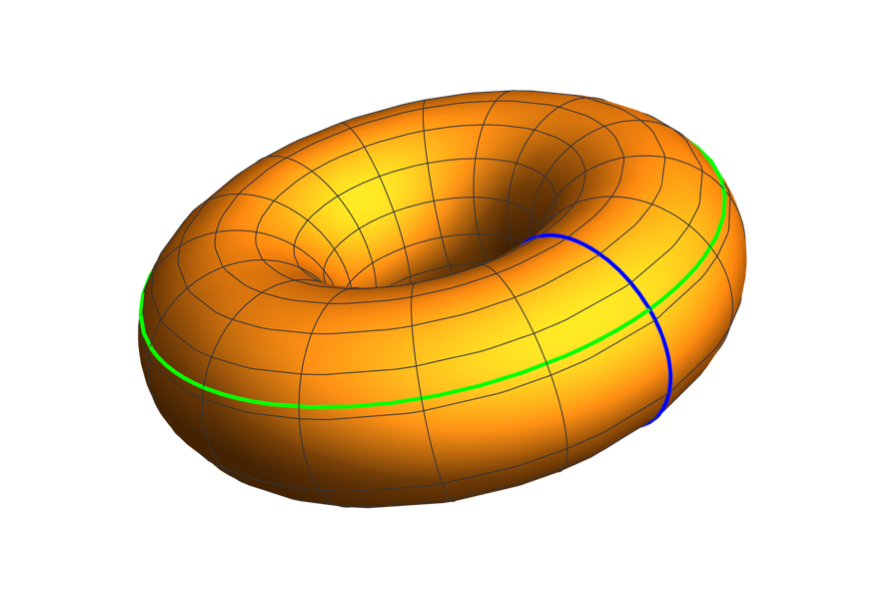
\includegraphics[width=\linewidth]{sup2}
	\end{subfigure}
\end{figure}
\section{Primera forma fundamental}
La primera forma fundamental es una matriz dada por los productos interiores de los vectores tangentes básicos $\mathbf{x}_u$ y $\mathbf{x}_v$. De acuerdo a la expresión
\begin{align*}
	\langle v,w\rangle=&\langle a\mathbf{x}_u+b\mathbf{x}_v,c\mathbf{x}_u+d\mathbf{x}_v\rangle\\
	=&\langle a\mathbf{x}_u,c\mathbf{x}_u+d\mathbf{x}_v\rangle+\langle b\mathbf{x}_v,c\mathbf{x}_u+d\mathbf{x}_v\rangle\\
	=&\langle a\mathbf{x}_u,c\mathbf{x}_u\rangle+\langle a\mathbf{x}_u,d\mathbf{x}_v\rangle+\langle b\mathbf{x}_v,c\mathbf{x}_u\rangle+\langle b\mathbf{x}_v,d\mathbf{x}_v\rangle\\
	=&ac\langle\mathbf{x}_u,\mathbf{x}_u\rangle+(ad+cd)\langle\mathbf{x}_u,\mathbf{x}_v\rangle+bd\langle\mathbf{x}_v,\mathbf{x}_v\rangle
\end{align*}
para dos vectores tangentes $v$ y $w$, sabemos que todas las propiedades métricas de los vectores tangentes están determinadas por la primera forma fundamental. Si ponemos
\[I=\begin{pmatrix}\langle\mathbf{x}_u,\mathbf{x}_u\rangle&\langle\mathbf{x}_u,\mathbf{x}_v\rangle\\\langle\mathbf{x}_u,\mathbf{x}_v\rangle&\langle\mathbf{x}_v,\mathbf{x}_v\rangle\end{pmatrix}=\begin{pmatrix}E&F\\F&G\end{pmatrix}\]
entonces
\[\langle v,w\rangle=v^TIw=acE+(ad+cd)F+bdG\]
¿Cómo calculamos longitudes de arco usando el lenguaje de la primera forma fundamental? La idea aquí es usar  una curva en la superficie que se obtiene tomando una curva en el dominio de la parametrización y luego levantándola a la superficie.
\section{Longitudes de curvas}
Tomemos una curva $\beta(t)=(u(t),v(t))$ en el dominio de una parametrización local, y definamos  nuestra curva por $\alpha(t)=(\mathbf{x}\circ\beta)(t)=\mathbf{x}(u(t),v(t))$.

Naturalmente, queremos que la longitud de la curva en la superficie $\alpha$ sea
\[\ell(\alpha)=\int_{t_0}^{t_1}|\alpha'(t)|dt\]
Así que nos interesa calcular
\begin{align*}
	\alpha'(t)=d_{\beta(t)}\mathbf{x}\cdot\beta'(t)
	=\begin{pmatrix}\frac{\partial\mathbf{x}^1}{\partial u}&\frac{\partial\mathbf{x}^1}{\partial v}\\\frac{\partial\mathbf{x}^2}{\partial u}&\frac{\partial\mathbf{x}^2}{\partial v}\\\frac{\partial\mathbf{x}^3}{\partial u}&\frac{\partial\mathbf{x}^3}{\partial v}\end{pmatrix}_{\beta(t)}\begin{pmatrix}u'(t)\\ \\v'(t)\end{pmatrix}
	=\begin{pmatrix}\frac{\partial\mathbf{x}^1}{\partial u}\big|_{\beta(t)}u'(t)+\frac{\partial\mathbf{x}^1}{\partial v}\big|_{\beta(t)}v'(t)\\\frac{\partial\mathbf{x}^2}{\partial u}\big|_{\beta(t)}u'(t)+\frac{\partial\mathbf{x}^2}{\partial v}\big|_{\beta(t)}v'(t)\\\frac{\partial\mathbf{x}^3}{\partial u}\big|_{\beta(t)}u'(t)+\frac{\partial\mathbf{x}^3}{\partial v}\big|_{\beta(t)}v'(t)\end{pmatrix}
\end{align*}
Que es de hecho igual a $u'(t)\mathbf{x}_u(\beta(t))+v'(t)\mathbf{x}_v(\beta(t))$.

Cuando claculamos la norma aparece la primera forma fundamental (quitamos la $t$ y la $\beta(t)$ para facilitar la escritura):
\begin{align*}
	|\alpha'|^2=&\langle \alpha',\alpha'\rangle\\
	=&\langle u'\mathbf{x}_u+v'\mathbf{x}_v ,u'\mathbf{x}_u+v'\mathbf{x}_v\rangle\\
	=&\langle u'\mathbf{x}_u+,u'\mathbf{x}_u+v'\mathbf{x}_v\rangle+\langle v'\mathbf{x}_v,u'\mathbf{x}_u+v'\mathbf{x}_v\rangle\\
	=&\langle u'\mathbf{x}_u,u'\mathbf{x}_v\rangle+\langle u'\mathbf{x}_u,v'\mathbf{x}_v\rangle+\langle v'\mathbf{x}_u+u'\mathbf{x}_v\rangle+\langle v'\mathbf{x}_u+v'\mathbf{x}_v\rangle\\
	=&(u')^2\langle\mathbf{x}_u+\mathbf{x}_v\rangle+2u'v'\langle \mathbf{x}_u,\mathbf{x}_v\rangle+(v')^2\langle \mathbf{x}_v,\mathbf{x}_v\rangle\\
\end{align*}
O sea que a la mera hora
\begin{align*}
	\ell(\alpha)=&\int_{t_0}^{t_1}|\alpha'(t)|dt\\
	=&\int_{t_0}^{t_1}\sqrt{Eu'^2+2Fu'v'+Gv'^2}dt
\end{align*}
\begin{ejem}[longitudes de curvas en el toro]
	Primero debemos calcular la primera forma fundamental, para lo cual calculamos los vectores tangentes básicos de acuerdo a la parametrización local que dimos arriba:
	\[\mathbf{x}(\varphi,\theta)=(\cos\theta(a+r\cos{\varphi}),\sin\theta(a+r\cos\varphi),r\sin\varphi)\]
	Derivando obtenemos:
	\[\mathbf{x}_\varphi=(r\cos{\theta}\sin{\varphi},-r\sin{\theta}\sin{\varphi},r\cos{\varphi})\\
	\mathbf{x}_\theta=(-\sin{\theta}(a+r\cos{\varphi}),\cos{\theta}(a+r\cos{\varphi}),0)\]
	Luego, los productos internos son
	\begin{align*}
		E=\langle\mathbf{x}_\varphi,\mathbf{x}_\varphi\rangle=&r^2\cos^2{\theta}\sin^2{\varphi}+r^2\sin^2{\theta}\sin^2{\varphi}+r^2\cos^2{\varphi}\\
		=&r^2(\cos^2{\theta}\sin^2{\varphi}+\sin^2{\theta}\sin^2{\varphi}+\cos^2{\varphi})\\
		=&r^2(\sin^2{\varphi}(\cos^2{\theta}+\sin^2{\theta})+\cos^2{\varphi})\\
		=&r^2\\\\
		F=\langle\mathbf{x}_\varphi,\mathbf{x}_\theta\rangle=&r\cos{\theta}\sin{\varphi}(-\sin{\theta}(a+r\cos{\varphi}))+...\\=&0\\\\
		G=\langle\mathbf{x}_\theta,\mathbf{x}_\theta\rangle=&\sin^2\theta(a+r\cos{\varphi})^2+\cos^2{\theta}(a+r\cos{\varphi})^2\\
		=&(a+r\cos{\varphi})^2
	\end{align*}
	Y ahora simplemente usamos la idea de la sección anterior para una curva en el toro.
	
	Por ejemplo, tomemos la curva $\beta(t)=(u(t),v(t))=(t,2t)$ definida en el dominio de nuestra parametrización, que es un cuadrado de lado $2\pi$. Derivando, obtenemos que $u'=1$ y $v'=2$, de forma que  la longitud de la curva $\alpha=\mathbf{x}\circ\beta$ está dada por
	\begin{align*}
		\int_{t_0}^{t_1}|\alpha'(t)|dt=&\int_{t_0}^{t_1}\sqrt{I(\alpha'(t))}dt\\
		=&\int_{t_0}^{t_1}\sqrt{Eu'^2+2Fu'v'+Gv'^2}dt\\
		=&\int_{t_0}^{t_1}\sqrt{r^2+2(a+r\cos{\varphi})^2}dt
	\end{align*}
	Escogiendo un toro canónico, digamos $a=2$, $r=1$, obtenemos
	\begin{align*}
		\int_{t_0}^{t_1}|\alpha'(t)|=&\int_{t_0}^{t_1}\sqrt{1+2(2+\cos{2t})^2}dt\\
		=&\int_{t_0}^{t_1}\sqrt{1+2(4+2\cos{2t}+\cos^2{2t})}dt\\
		=&\int_{t_0}^{t_1}\sqrt{5+4\cos{2t}+2\cos^2{2t})}dt\\
		=&\qquad?
	\end{align*}
\end{ejem}
\begin{figure}[H]
	\begin{subfigure}{0.5\textwidth}
		\centering
		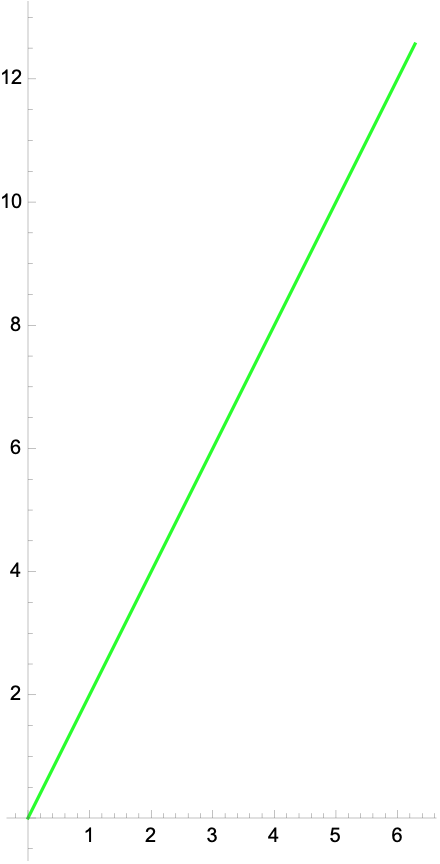
\includegraphics[width=0.5\linewidth]{sup3}
	\end{subfigure}
	\begin{subfigure}{0.5\textwidth}
		\centering
		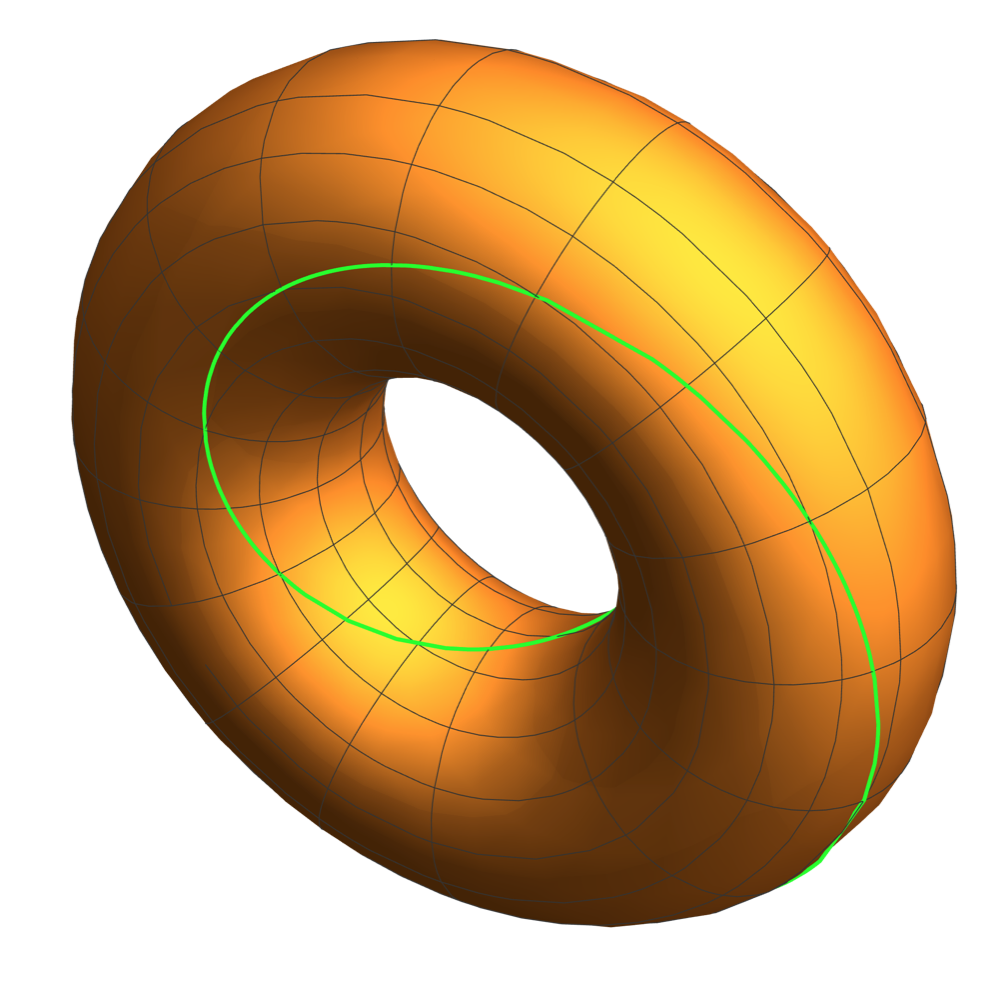
\includegraphics[width=0.7\linewidth]{sup4}
	\end{subfigure}
\end{figure}
\begin{ejem}[La recta identidad en la esfera]
	No es una coincidencia que la integral del ejemplo anterior sea complicada. De hecho, hay muchas curvas sencillas cuya longitud está dada por una integral no trivial, en algunos casos incluso elíptica (la recta identidad levantada a la esfera).	
	\begin{figure}[H]
		\begin{subfigure}{0.5\textwidth}
			\centering
			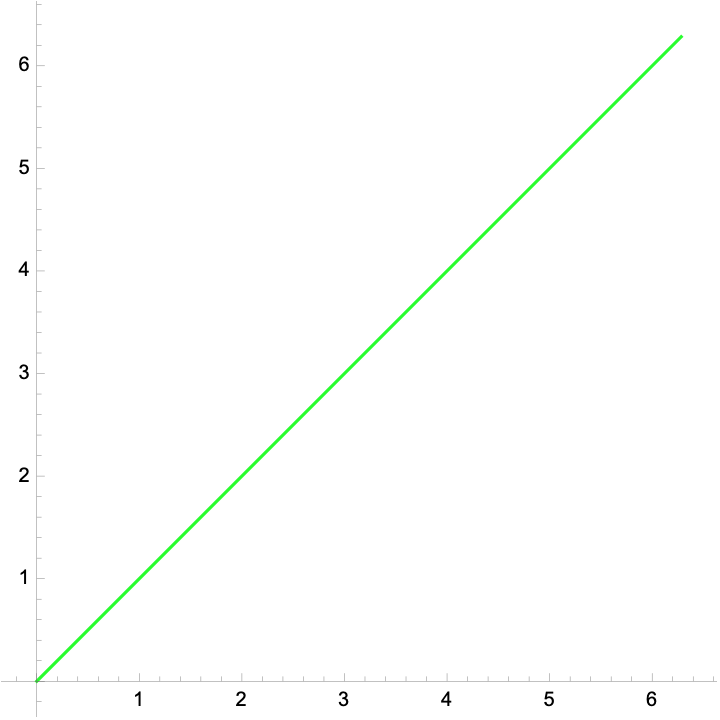
\includegraphics[width=0.7\linewidth]{sup5}
		\end{subfigure}
		\begin{subfigure}{0.5\textwidth}
			\centering
			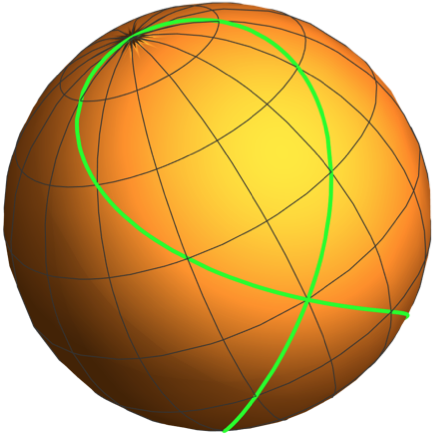
\includegraphics[width=0.7\linewidth]{sup6}
		\end{subfigure}
	\end{figure}
\end{ejem}
\section{Áreas}
Intuitivamente, queremos que el área de una región esté dada por el área de ciertos paralelogramos infinitesimales en cada punto de la región. Pensando en usar la parametrización local de nuestra superficie, queremos integrar el área del paralelogramo infinitesimal generado por los vectores tangentes básicos en cada punto.

Así que si $Q$ es una región (subconjunto compacto cuya frontera es una curva cerrada regular salvo por una cantidad finita de puntos) en el dominio de alguna parametrización local, definimos el área de la región en la superficie $\mathbf{x}(Q):=R$ como
\[A(R)=\iint_Q|\mathbf{x}_u\wedge\mathbf{x}_v|dudv\]
donde $|\mathbf{x}_u\wedge\mathbf{x}_v|$ es el área del paralelogramo generado por los vectores $\mathbf{x}_u$ y $\mathbf{x}_v$.

Esta notación proviene de un objeto muy general que se llama "álgebra exterior", que es una estructura algebraica donde está bien definido el producto cuña $\wedge$ entre sus elementos. Aunque $\mathbf{x}_u$ y $\mathbf{x}_v$ son vectores en $\R^3$, el producto cuña de ellos no. Esta álgebra es una estructura fundamental para la teoría de integración en variedades de cualquier dimensión.

Para nuestro caso, recordemos de geometría analítica que de hecho el área del paralelogramo generado por dos vectores en $\R^3$ es la magnitud de su producto curuz, es decir, $|\mathbf{x}_u\wedge\mathbf{x}_v|=|\mathbf{x}_u\times\mathbf{x}_v|$, que podríamos tomarlo como definición. Este resultado se debe a que:
\begin{figure}[H]
	\centering
	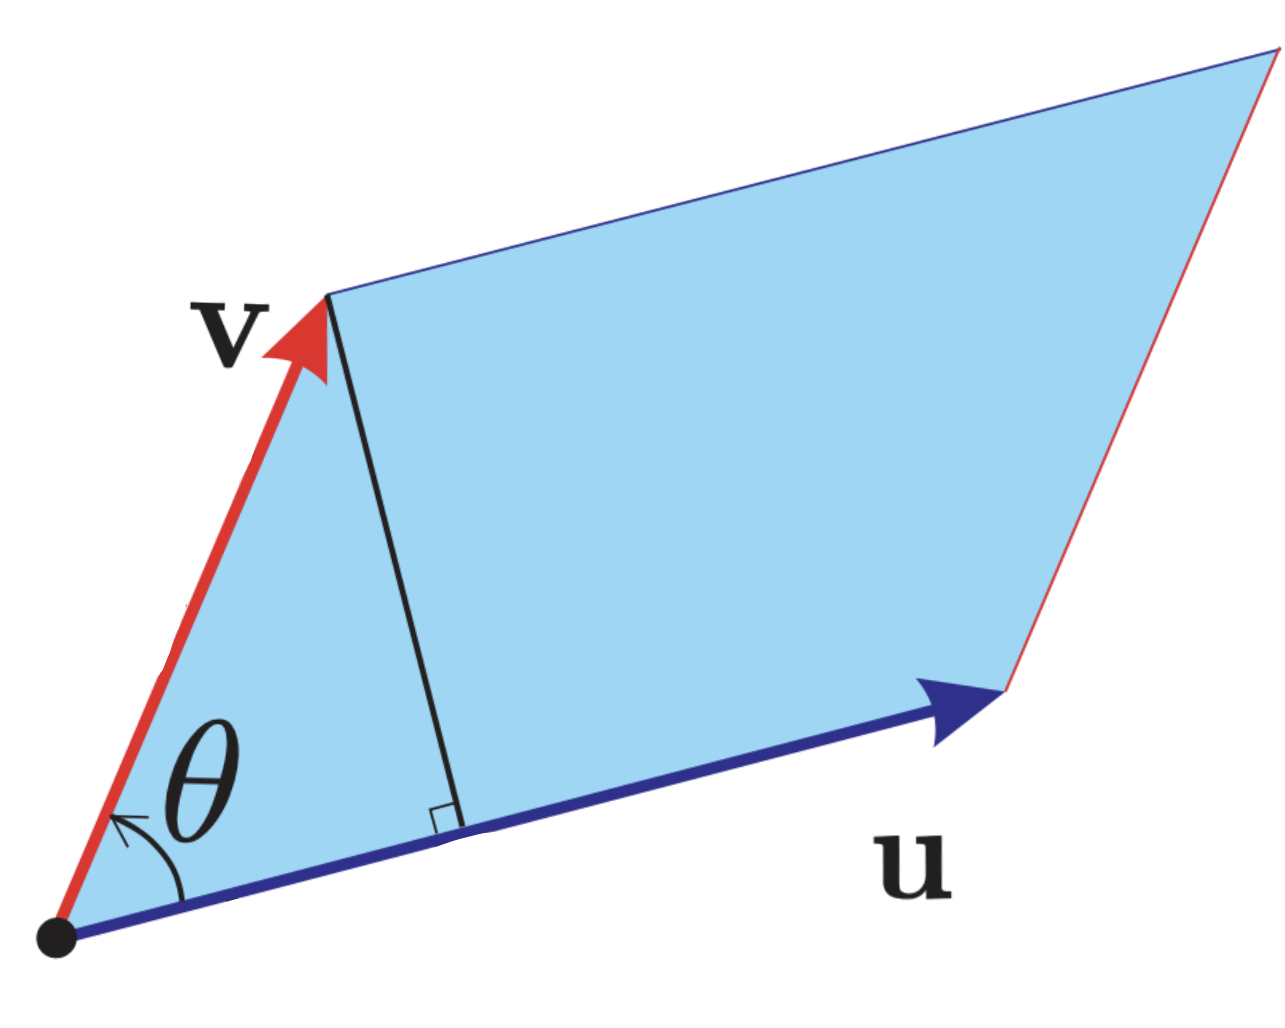
\includegraphics[width=0.4\linewidth]{sup7}
\end{figure}
(Consultar en Bracho, Introducción analítica a las geometrías) el área de un paralelogramo es base por altura, y la altura del paralelogramo generado por $\mathbf{u}$ y $\mathbf{v}$ es $|\mathbf{v}|\sin{\theta}$ de acuerdo al diagrama. Y bueno, una propiedad del producto cruz es que $|\mathbf{u}\times\mathbf{v}|=|\mathbf{u}||\mathbf{v}|\sin{\theta}$, para el ángulo $\theta\in[0,\pi]$ entre los vectores.

Con todo esto en mente, Do Carmo nos hace notar que 
\begin{align*}
	|\mathbf{x}_u\wedge\mathbf{x}_v|^2+\langle\mathbf{x}_u,\mathbf{x}_v\rangle^2=&|\mathbf{x}_u\times\mathbf{x}_v|^2+\langle\mathbf{x}_u,\mathbf{x}_v\rangle^2\\
	=&|\mathbf{x}_u|^2|\mathbf{x}_v|^2\sin^2{\theta}+|\mathbf{x}_u|^2|\mathbf{x}_v|^2\cos^2{\theta}\\
	=&|\mathbf{x}_u|^2|\mathbf{x}_v|^2
\end{align*}
Y entonces
\begin{align*}
	|\mathbf{x}_u\wedge\mathbf{x}_v|^2=&|\mathbf{x}_u|^2|\mathbf{x}_v|^2-\langle\mathbf{x}_u,\mathbf{x}_v\rangle^2\\
	=&\langle\mathbf{x}_u,\mathbf{x}_u\rangle\langle\mathbf{x}_v,\mathbf{x}_v\rangle-\langle\mathbf{x}_u,\mathbf{x}_v\rangle^2\\
	=&EG-F^2
\end{align*}
Así que por fin volvió a aparecer la primera forma fundamental. Hemos visto que
\[A(R)=\iint_Q\sqrt{EG-F^2}dudv\]
Como en el caso de las longitudes de curvas, sólo necesitamos saber cómo son las cosas *en el dominio de la parametrización* y no directamente en la superficie.

\begin{ejem}[El área del toro. Ejemplo 5, cap 2, Do Carmo]
	Ya hemos hecho casi todo el trabajo. Aunque se nos antoja integrar en todo el cuadrado $C=(0,2\pi)\times(0,2\pi)$ que sea el dominio una parametrización local, no podemos hacerlo directamente porque nuestra definición de integral está dada en conjuntos compactos. Así, debemos tomar un cuadrado un poquitito más pequeño: $C_\varepsilon=[0+\varepsilon,2\pi-\varepsilon]\times[0+\varepsilon,2\pi-\varepsilon]$.
	
	Aquí sí integramos:
	\begin{align*}
		A(T)=&\iint_{C_\varepsilon}\sqrt{EG-F^2}dudv\\
		=&\iint_{C_\varepsilon}r(a+r\cos{u})dudv\\
		=&\int_{\varepsilon}^{2\pi-\varepsilon}(ra+r^2\cos{u})du\int_{\varepsilon}^{2\pi-\varepsilon}dv\\
		=&\big(\big[rau\big]_{\varepsilon}^{2\pi-\varepsilon}+\big[r^2\sin{u}\big]_{\varepsilon}^{2\pi-\varepsilon}\big)(2\pi-2\varepsilon)^2\\
		=&\big(ra(2\pi-\varepsilon)-ra\varepsilon+r^2\sin{(2\pi-\varepsilon)}-r^2\sin{\varepsilon}\big)(2\pi-2\varepsilon)^2
	\end{align*}
	que cuando $\varepsilon\to0$ se vuelve $4\pi^2ra$.
\end{ejem}
\section{Isometrías}
Primero revisemos las definiciones de Do Carmo:
\begin{defn}[Función real diferenciable]
	Una función $f:V\subseteq S\to \R$ es diferenciable en $p\in v$ si existe una parametrización local $\mathbf{x}$ de $p$ tal que la composición $f\circ\mathbf{x}$ sea diferenciable
\end{defn}
\begin{defn}[Función diferenciable entre superficies]
	Decimos que $\varphi:S\to\bar{S}$ es diferenciable si existen parametrizaciones locales $\mathbf{x}$ y $\mathbf{y}$ de las superficies tales que la composición $\mathbf{y}\circ f\circ\mathbf{x}^{-1}$ es diferenciable.
\end{defn}
Quizás podemos dispensar de estas dos definiciones y usar la diferenciabilidad en $\R^3$... Sea como sea, definimos
\begin{defn}[Isometría]
	Una función $\varphi:S\to\bar{S}$ es una isometría si es un difeomorfismo (función diferenciable con inversa diferenciable) y preserva la primera forma fundamental, es decir, si para cualquesquiera vectores tangentes $u$ y $v$ a $S$, se tiene que
	$$
	\langle u,v\rangle_p=\langle d_p\varphi v,d_p\varphi v\rangle_{\varphi(p)}
	$$
\end{defn}
\begin{defn}[Isometría local]
	Una función $\varphi:S\to\bar{S}$ es una isometría local si para cada punto $p\in S$ existen vecindades $V$ de $p$ y $\bar{V}$ de $\varphi(p)$ tales que la restricción $\varphi|_{V}:V\to\bar{V}$ es una isometría.
\end{defn}
\begin{prop}
	Una función $\varphi:S\to\bar{S}$ es una isometría local si para cada punto $p\in S$ existen vecindades $V$ de $p$ y $\bar{V}$ de $\varphi(p)$ tales que la restricción $\varphi|_{V}:V\to\bar{V}$ es una isometría.
\end{prop}
\begin{prop}
	Si existen dos parametrizaciones locales $\mathbf{x}$ y $\bar{\mathbf{x}}$ de $S$ y $\bar{S}$ tales que $E=\bar{E}$, $F=\bar{F}$ y $G=\bar{G}$, entonces la aplicación $\varphi=\mathbf{\bar{x}\circ\mathbf{x}^{-1}}:\mathbf{x}(U)\to\bar{S}$ es una isometría local.
\end{prop}
\begin{prop}[Recíproca]\label{prop:reciproca}
	Sea $\varphi:S\to\bar S$ una isometría y $\mathbf x:U\to S$ una parametrización en $p\in S$. Entonces, la función $\bar{\mathbf x}=\varphi\circ\mathbf{x}$  es una parametrización local en $\varphi(p)$ tal que $E=\bar{E}$, $F=\bar{F}$ y $G=\bar{G}$.
\end{prop}
\begin{ejem}[la catenoide y la helicoide. Ejemplo 2, Cap. 4, Do Carmo]
	La catenoide es la superficie de revolución que se obtiene rotando la curva $\alpha(t)=(0,\cosh{t},t)$ alrededor del eje $Z$. Todas sus propiedades se obtienen análogamente a lo que se hizo con el toro. Siguiendo a Do Carmo, la parametrización está dada por
	\[\mathbf{x}(u,v)= (a\cosh{v}\cos{u},a\cosh{v}\sin{v},av)\]
	para algún parámetro $a$. Con nuestro código en Mathematica, tomando $a=1$, obtenemos
	\[\mathbf{x}(u,v)= (\cosh{v}\sin{u},\cosh{v}\cos{v},v)\]
	Por otro lado, la helicoide está parametrizada por
	\[\bar{\mathbf{x}}(\bar{u},\bar{v})= (\bar{u}\cos{v},\bar{u}\sin{\bar{v}},a\bar{v})\]
	\begin{figure}[H]
		\begin{subfigure}{0.5\textwidth}
			\centering
			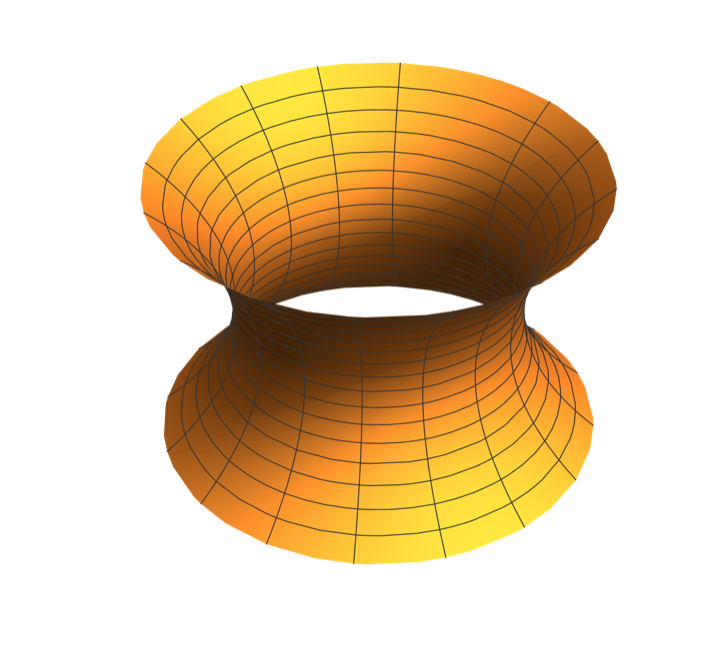
\includegraphics[width=0.9\linewidth]{sup8}
		\end{subfigure}
		\begin{subfigure}{0.5\textwidth}
			\centering
			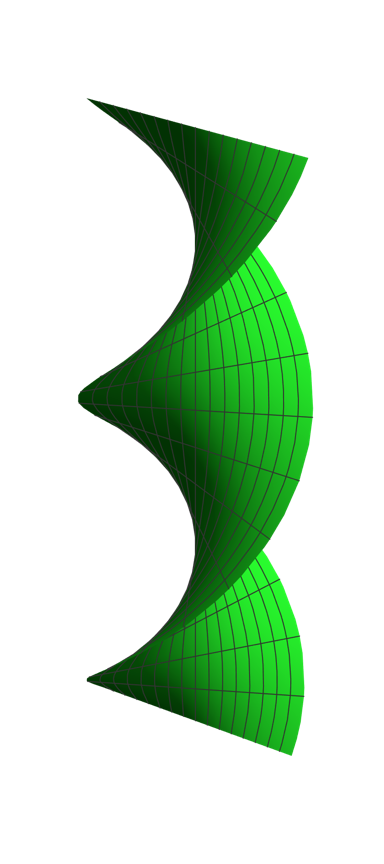
\includegraphics[width=0.4\linewidth]{sup9}
		\end{subfigure}
	\end{figure}
\end{ejem}
Ahora para ver que las dos superficies son isométricas es suficiente, por la proposición anterior, ver que cada una tiene una parametrización tal que los coeficientes de la primera forma fundamental de cada una sean iguales.

Usando nuestro código de Mathematica podemos comprobar que esto no sucede para las dos parametrizaciones que acabamos de dar. Luego, hay que reparametrizar alguna de las superficies. Do Carmo lo hace para la helicoide de acuerdo a la sustitución:
$$
\bar{u}=u,\qquad\bar{v}=a\sinh{v},\qquad 0<u<2,\quad-\infty<v<\infty
$$
que es una función biyectiva cuyo Jacobiano no se anula. Con esta parametrización, la primera forma fundamental de ambas superficies está dada por
$$
E=a^2\cosh^2{v},\qquad F=0,\qquad G=a^2\cosh^2v
$$
En el siguiente dibujo hecho en Mathematica vemos una deformación continua de una superficie en otra:
	\vspace{-.6cm}
	\begin{figure}[H]
		\begin{subfigure}{0.3\textwidth}
			\centering
			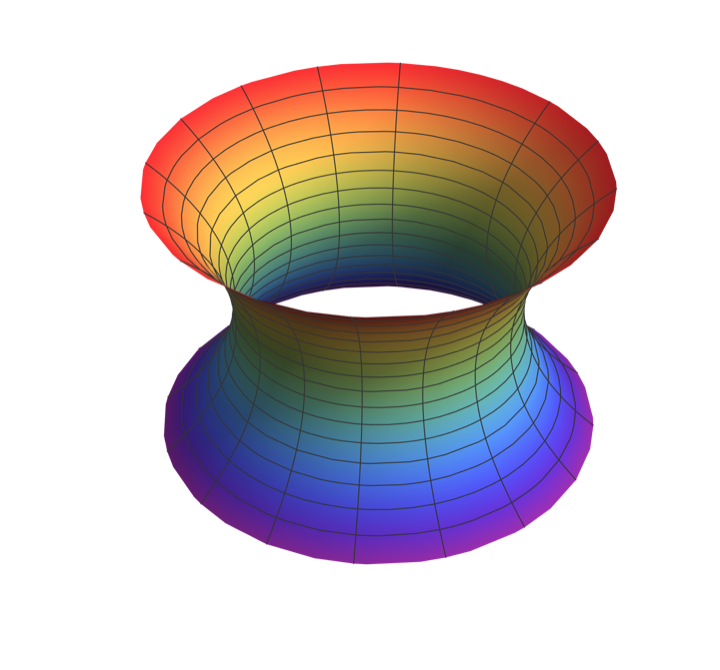
\includegraphics[width=\linewidth]{sup10}
		\end{subfigure}
		\begin{subfigure}{.2\textwidth}
			\centering
			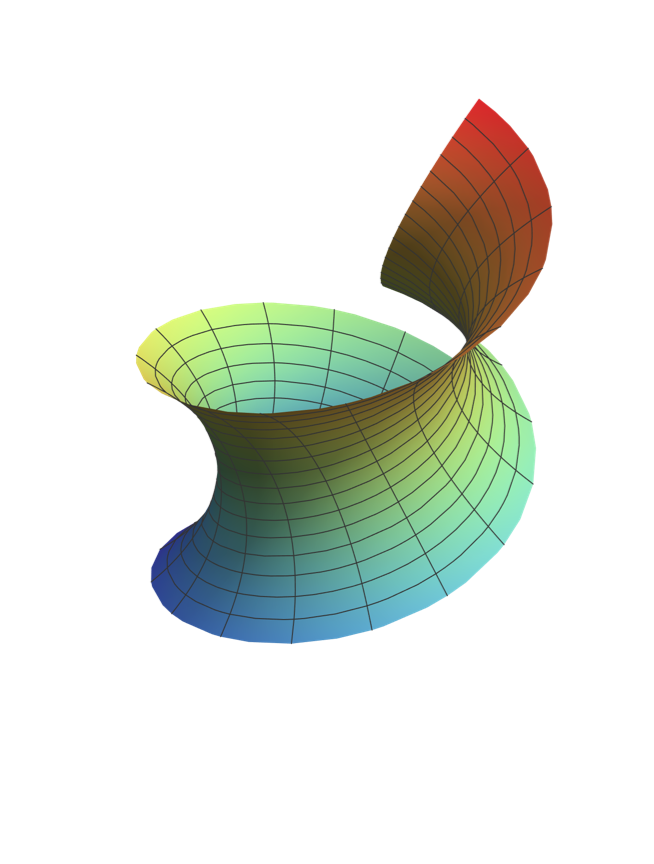
\includegraphics[width=\linewidth]{sup11}
		\end{subfigure}
		\begin{subfigure}{.2\textwidth}
			\centering
			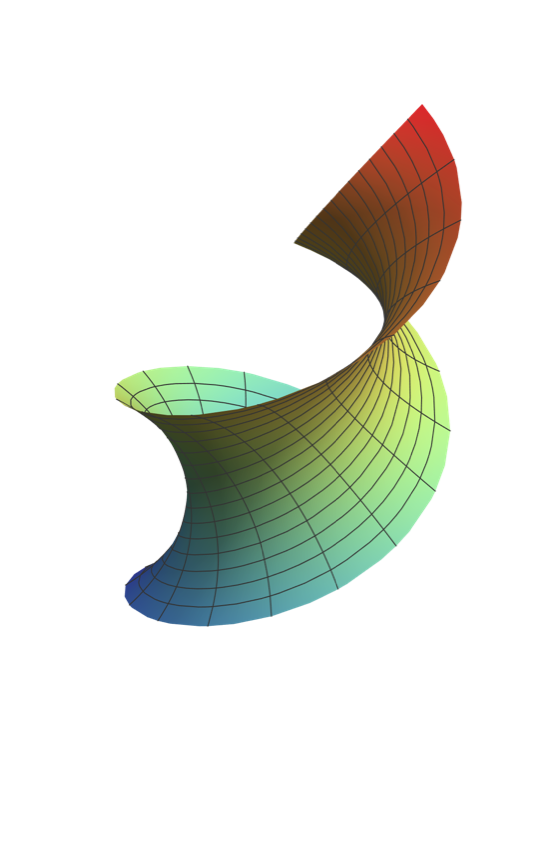
\includegraphics[width=\linewidth]{sup12}
		\end{subfigure}
		\begin{subfigure}{.125\textwidth}
			\centering
			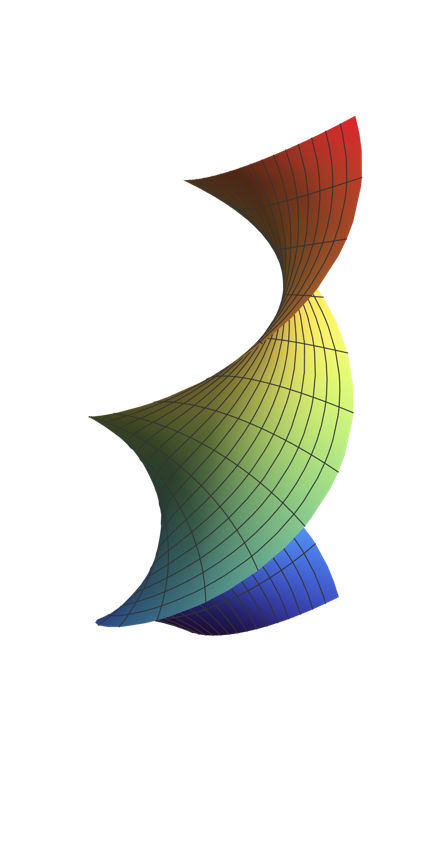
\includegraphics[width=\linewidth]{sup13}
		\end{subfigure}
		\begin{subfigure}{0.125\textwidth}
			\centering
			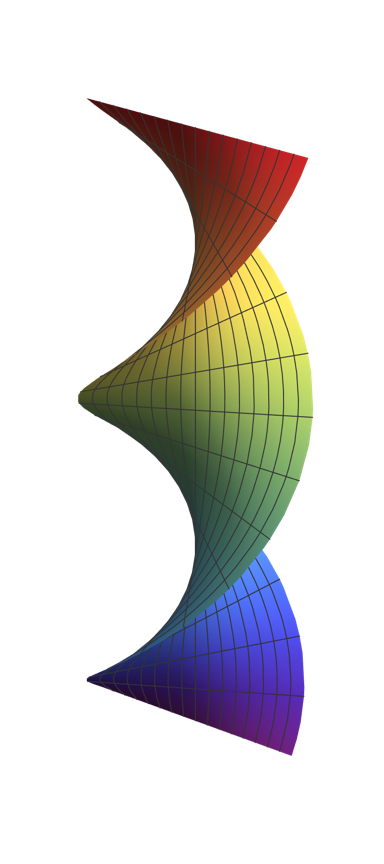
\includegraphics[width=\linewidth]{sup14}
		\end{subfigure}
	\end{figure}
	\vspace{-.6cm}
	Estos dibujos fueron creados usando una simple homotopía "de línea recta" entre las parametrizaciones, explícitamente dada por
	\[H(t,(u,v))=t\mathbf{x}(u,v)+(1-t)\bar{\mathbf{x}}(u,v)\]
	para $t\in[0,1]$.
	\begin{pregunta}[Hasta ahora sin respuesta]
		¿La homotopía preserva la estructura regular de las superficies? Es decir, ¿las superficies en los puntos de en medio son todas regulares? ¿Isométricas?
	\end{pregunta}
	
\begin{ejer}[El cono y el Pac-Man. Ejemplo 2, Cap. 4, Do Carmo] Mostrar que el cono visto como superficie de revolución y el Pac-Man no tienen la misma primera forma fundamental. Usar la parametrización que da Do Carmo y comprobar que de esa forma sí coincide la primera forma fundamental.
		\vspace{-2cm}
		\begin{figure}[H]
		\begin{subfigure}{0.5\textwidth}
			\centering
			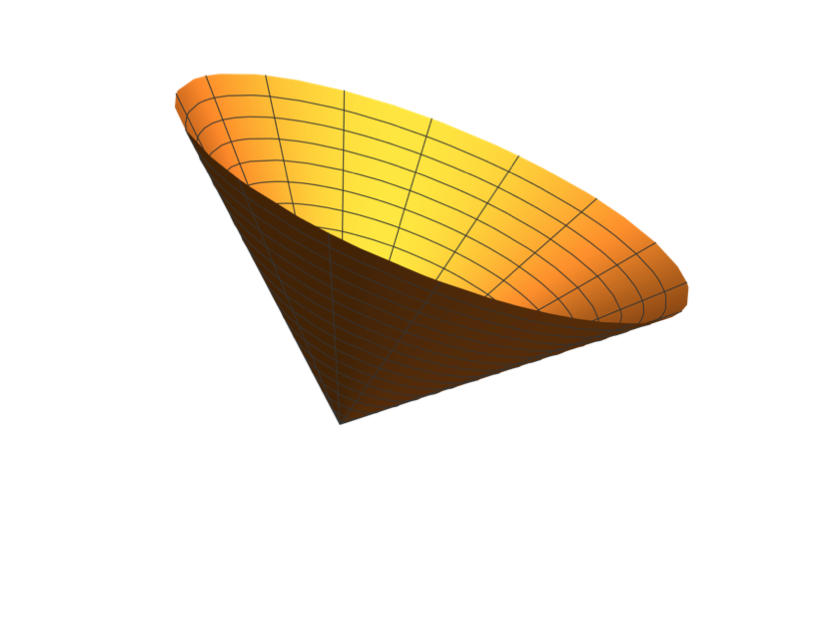
\includegraphics[width=\linewidth]{sup15}
		\end{subfigure}	\hspace{-1cm}
		\begin{subfigure}{.5\textwidth}
			\centering
			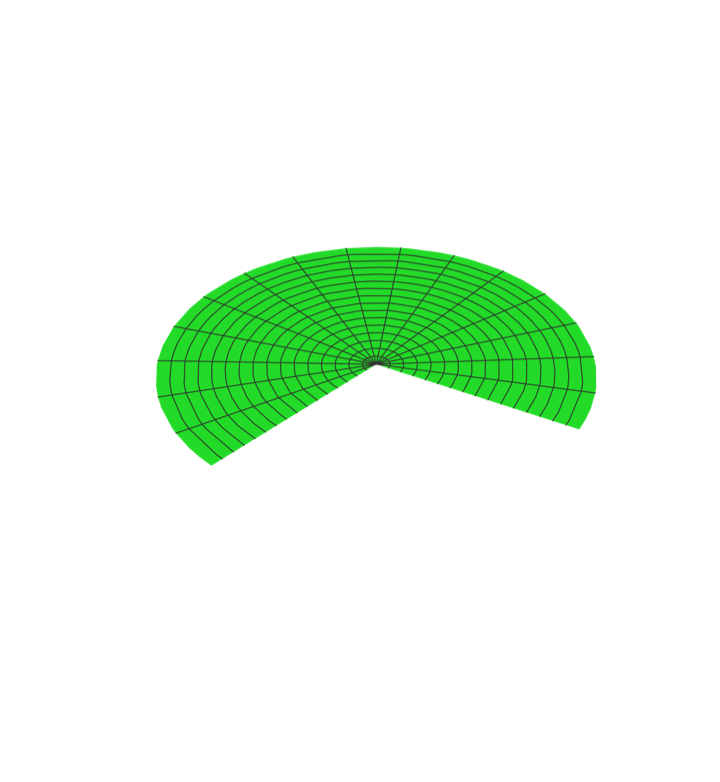
\includegraphics[width=\linewidth]{sup16}
		\end{subfigure}
	\end{figure}
	\vspace{-2cm}
	\begin{figure}[H]
		\begin{subfigure}{.3\textwidth}
			\centering
			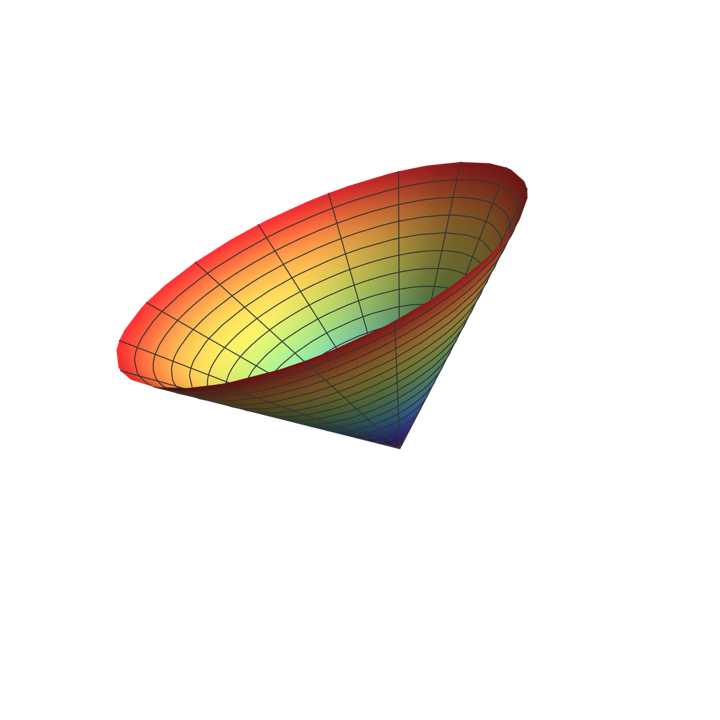
\includegraphics[width=\linewidth]{sup17}
		\end{subfigure}	\hspace{-1.2cm}
		\begin{subfigure}{.3\textwidth}
			\centering
			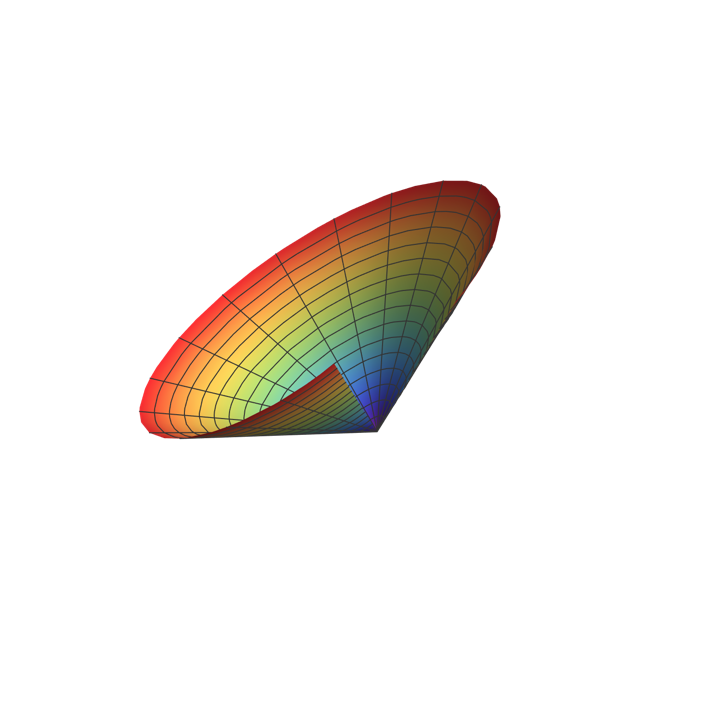
\includegraphics[width=\linewidth]{sup18}
		\end{subfigure}	\hspace{-1.2cm}
		\begin{subfigure}{.3\textwidth}
			\centering
			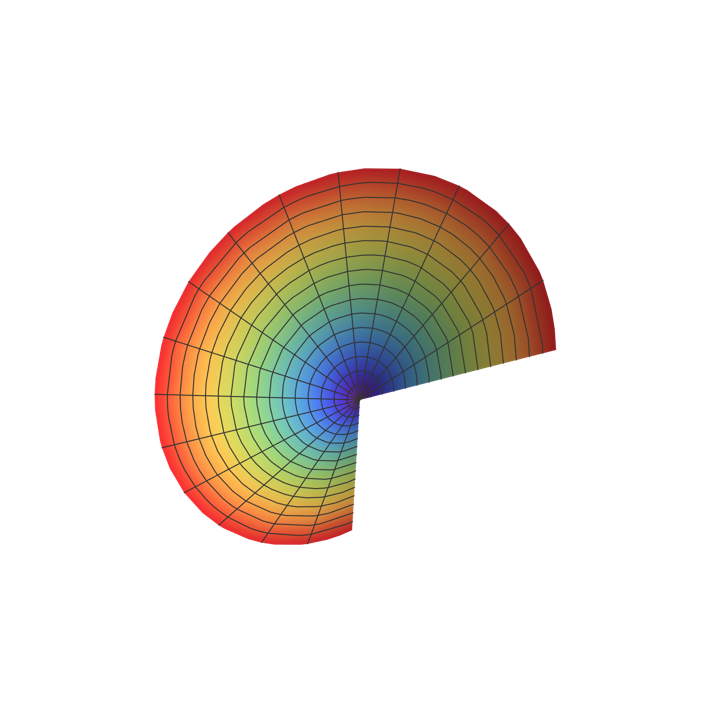
\includegraphics[width=\linewidth]{sup19}
		\end{subfigure}	\hspace{-1cm}
		\begin{subfigure}{.3\textwidth}
			\centering
			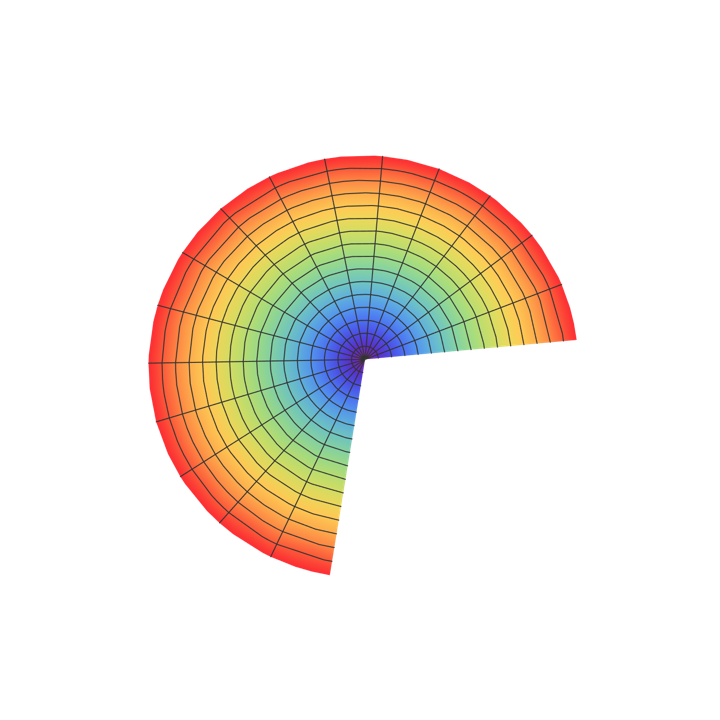
\includegraphics[width=\linewidth]{sup20}
		\end{subfigure}
	\end{figure}
\end{ejer}
\begin{proof}[Solución]
	Primero, ¿cuál es una parametrización del cono?
	
	Bueno, tomamos una línea con pendiente $\varphi$ en el plano $yz$ y rotémosla:
	\begin{align*}
		\alpha:\R&\to\R^3\\
		t&\mapsto(0,t,\varphi t)
	\end{align*}
	Recordemos que la matriz de rotación alrededor del eje $z$ por ángulo $\theta$, denotada por $R_\theta$, es tal que
	\begin{align*}
		e_1&\xrightarrow{R_\theta} (0,\cos\theta,\sin\theta)\\
		e_2&\xrightarrow{R_\theta}(0,-\sin\theta,\cos\theta)\\
		e_3&\xrightarrow{R_\theta}e_3
	\end{align*}
	así que
	\[R_\theta=\begin{pmatrix}\cos\theta&-\sin\theta&0\\ \sin\theta&\cos\theta&0\\0&0&1\end{pmatrix}\]
	Luego, los puntos en el cono son de la forma
	\[\mathbf{x}(t,\theta)=R_\theta\cdot\alpha(t)=\begin{pmatrix}\cos\theta&-\sin\theta&0\\ \sin\theta&\cos\theta&0\\0&0&1\end{pmatrix}\begin{pmatrix}0\\t\\\varphi t\end{pmatrix}=\begin{pmatrix}-t\sin\theta\\\cos\theta\\\varphi t\end{pmatrix}\]
	Parece bien. Ahora parametricemos el Pac-Man que corresponde. Aquí hay que hacer algo de geometría clásica. El meollo del asunto es la siguiente relación
	\begin{figure}[H]
		\centering
		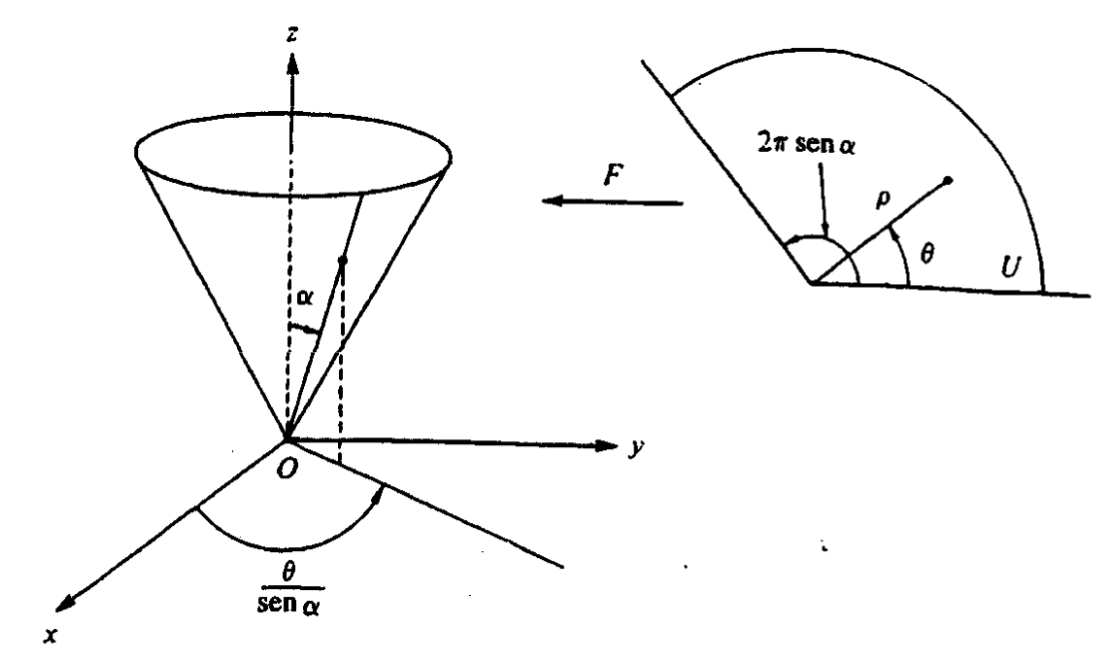
\includegraphics[width=0.5\linewidth]{sup21}
	\end{figure}
	De acuerdo al diagrama, $\sin\alpha$ es el tamaño del lado opuesto del triángulo rectángulo con lado ayacente al eje $z$ e hipotenusa sobre el cono, cuando la hipotenusa mide 1. Esta cantidad es el radio de un círculo que se obtiene al cortar el cono con un plano paralelo a $xy$. Específicamente, ese círculo es
	\[\{(\sin\alpha\cos\theta,\sin\alpha\sin{{\theta}},\cos\alpha)\in\R^3|\theta\in[0,2\pi]\}\]
	Cuando desenrollamos el cono para convertirlo en el Pac-Man, queremos que ese círculo, cuya circunferencia mide $2\pi\sin\alpha$ sea el tamaño del sector de circunferencia del Pac-Man.
	
	Una vez establecido esto, tenemos la parametrización del Pac-Man
	\[\mathbf{\bar{x}}(u,v)=(u\cos{v},u\sin v,0),\qquad u\in\R^+,v\in(0,2\pi\sin\alpha)\]
	donde, de acuerdo al dibujo $\alpha=\pi/2–\varphi$.
	
	Ahora toca calcular las primera formas fundamentales. Primero los vectores tangentes básicos:
	\begin{align*}
		\mathbf{x}_t&=(-\sin\theta,0,t)\\
		\mathbf{x}_\theta&=(-t\cos\theta,-\sin\theta,0)\\ \\
		\mathbf{\bar{x}}_u&=(\cos{v},\sin{v},0)\\
		\mathbf{\bar{x}}_v&=(-u\sin{v},u\cos{v},0)
	\end{align*}
	Y ahora sí
	\begin{align*}
		{E}&=\langle \mathbf{{x}}_u,\mathbf{{x}}_u\rangle=\sin^2{\theta}+t^2\\
		{F}&=\langle \mathbf{{x}}_u,\mathbf{{x}}_v\rangle=0\\
		{G}&=\langle \mathbf{{x}}_v,\mathbf{{x}}_v\rangle=t^2\sin^2{\theta}+\sin^2{\theta}\\\\
		\bar{E}&=\langle \mathbf{\bar{x}}_u,\mathbf{\bar{x}}_u\rangle=\cos^2{v}+\sin^2{v}=1\\
		\bar{F}&=\langle \mathbf{\bar{x}}_u,\mathbf{\bar{x}}_v\rangle=-u\cos{v}\sin{v}+u\cos{v}\sin{v}=\cos{v}\sin{v}(-u+u)=0\\
		\bar{G}&=\langle \mathbf{\bar{x}}_v,\mathbf{\bar{x}}_v\rangle=u^2\sin^2{v}+u^2\cos^2{v}=u^2\\
	\end{align*}
	Bueno, no pueden ser iguales porque $\bar{E}$ es constante y $E$ no. Resulta que hay una reparametrización del cono en términos del ángulo $\alpha=\pi/2-\varphi$:
	\[\mathbf{x}(\rho,\theta)=(\rho\sin\alpha\cos{\frac{\theta}{\sin{\alpha}}},\rho\sin\alpha\sin{\frac{\theta}{\sin{\alpha}}},\rho\cos\alpha)\]
	**¿Por qué?** Recordemos el círculo que nos ayudó a encontrar el ángulo del Pac-Man. Otra forma de definirlo es:
	\[\{(\sin\alpha\cos\frac{\theta}{\sin\alpha},\sin\alpha\sin{\frac{\theta}{\sin\alpha}},\cos\alpha)\in\mathbb{R}^3|\theta\in[0,2\pi\sin\alpha]\}\]
	Al multiplicar todo por $\rho$, estamos parametrizando círculos cuyos radios cambian proporcionalmente a la altura. Esto parametriza un nuestro cono.
	
	Para entender un poco más lo que dice Do Carmo, recordemos que el cono estándar es $\{(x,y,z)\in\mathbb{R}^3|x^2+y^2=z^2\}$. Dado el ángulo $\alpha$, nuestro cono es $\{(x,y,z)\in\mathbb{R}^3|x^2+y^2=(\frac{z}{\cot\alpha})^2\}$ **¿Por qué...?**.  Es decir necesitamos que $\cot{\alpha}\sqrt{x^2+y^2}=z$ para la parte de arriba del cono. Do Carmo nos muestra esta condición se satisface para los puntos de esta nueva parametrización:
	\[\cot\alpha\sqrt{x^2+y^2}=\cot\alpha\sqrt{\rho^2\sin^2\alpha}=\rho\cos\alpha=z\]
	Bueno… el chiste es que
	\begin{align*}
		\mathbf{x}_\rho&=(\sin\alpha\cos{\frac{\theta}{\sin{\alpha}}},\sin\alpha\sin{\frac{\theta}{\sin{\alpha}}},\cos\alpha)\\
		\mathbf{x}_\theta&=(-\rho\sin\alpha\sin\big({\frac{\theta}{\sin{\alpha}}}\big)\frac{1}{\sin\alpha},\rho\sin\alpha\cos\big({\frac{\theta}{\sin{\alpha}}}\big)\frac{1}{\sin\alpha},0)\\
		&=(-\rho\sin{\frac{\theta}{\sin{\alpha}}},\rho\cos{\frac{\theta}{\sin{\alpha}}},0) \\\\
		{E}&=\langle \mathbf{{x}}_\rho,\mathbf{{x}}_\rho\rangle=\sin^2\alpha\cos^2{\frac{\theta}{\sin{\alpha}}}+\sin^2\alpha\sin^2{\frac{\theta}{\sin{\alpha}}}+\cos^2\alpha=1\\
		{F}&=\langle \mathbf{{x}}_\rho,\mathbf{{x}}_\theta\rangle=0\\
		{G}&=\langle \mathbf{{x}}_\theta,\mathbf{{x}}_\theta\rangle=\rho^2
	\end{align*}
	Así es que sí son localmente isométricas. ¡Viva!
	
	Surge una pregunta importante: \textbf{¿Será que el truco para encontrar estas isometrías locales es que los dominios de las parametrizaciones sean iguales?} Tras un par de intentos en Mathematica, creo que la respuesta es que no.
\end{proof}

\section{Transformaciones conformes}
\begin{defn}
	Un \textbf{difeomorfismo} $\varphi:S\to\bar S$ es una transformación conforme si existe una función diferenciable $\lambda^2:S\to\mathbb{R}$ que nunca se anula tal que
	\[\langle u,v\rangle_p=\lambda^2(p)\langle d_p\varphi(u),d_p\varphi(v)\rangle_{\varphi(p)}\]
	para todo $p\in S$ y $u,v\in T_pS$.
	
	Para entender esta definición, tomemos dos curvas $\alpha$ y $\beta$ en $S$ que se intersecten en un punto $p=\alpha(0)=\beta(0)$. El ángulo entre ellas está dado por
	\[\cos\theta=\frac{\langle\alpha',\beta'\rangle_p}{|\alpha'||\beta'|}\]
	Y al aplicar nuestra transformación conforme obtenemos
	\[\cos\bar\theta=\frac{\langle d_p\varphi(\alpha'),d_p\varphi(\beta')\rangle_p}{|d_p\varphi(\alpha')||d_p\varphi(\beta')|}=\frac{\lambda^2(p)\langle\alpha',\beta'\rangle_p}{|\lambda\alpha'||\lambda\beta'|}=\frac{\langle\alpha',\beta'\rangle_p}{|\alpha'||\beta'|}=\cos\theta\]
	Tenemos una proposición análoga a la que nos permitió encontrar las isometrías de los ejemplos anteriores:
\end{defn}
\begin{prop}
	Si existen dos parametrizaciones locales $\mathbf{x}$ y $\bar{\mathbf{x}}$ de $S$ y $\bar{S}$ tales que $E=\lambda^2\bar{E}$, $F=\lambda^2\bar{F}$ y $G=\lambda^2\bar{G}$, entonces la aplicación $\varphi=\mathbf{\bar{x}\circ\mathbf{x}^{-1}}:\mathbf{x}(U)\to\bar{S}$ es una transformación conforme local.
\end{prop}
	Aquí, \textbf{transformación conforme local} significa que en cada punto de $S$ hay una vecindad donde la restricción de la transformación es conforme.
\begin{ejem}[La esfera y el plano mediante la proyección estereográfica]
	Para mostrar que el plano y la esfera son superficies conformes, usaremos la proyección estereográfica como parametrización local de la esfera, esto es:
	\begin{align*}
		\mathbf{x}:\mathbb{R}^2&\to S^2\backslash{N}\\
		(u,v)&\mapsto \left(\frac{2u}{1+u^2+v^2},\frac{2v}{1+u^2+v^2},\frac{-1+u^2+v^2}{1+u^2+v^2}\right)
	\end{align*}
	Definiendo $g=1+u^2+v^2$, tenemos que 
	\[\mathbf{x}(u,v)=\frac{1}{g}(2u,2v,u^2+v^2-1)\]
	Calculemos el primer vector tangente básico con la regla del producto:
	\begin{align*}
		\mathbf{x}_u&=\frac{1}{g}(2,0,2u)+\Big(\frac{-1}{g^2}\Big)(2u)(2u,2v,u^2+v^2-1)
	\end{align*}
	Notemos que la primera entrada aquí es
	\[\frac{2}{g}-\frac{4u^2}{g^2}=\frac{1}{g}\Big(2-\frac{4u^2}{g}\Big)=\frac{1}{g}\Big(\frac{2g-4u^2}{g}\Big)=\frac{2}{g^2}(g-2u^2)=\frac{2}{g^2}(-u^2+v^2+1)\]
	La segunda entrada es 
	\[\frac{2}{g^2}-2uv\]
	Y la tercera, ya buscando lo que creemos que puede ser el factor $\lambda^2$,
	\[\frac{2u}{g}-\frac{2u}{g^2}(u^2+v^2-1)=\frac{2}{g^2}\left(ug-u(u^2+v^2-1)\right)=\frac{2}{g^2}\left(u(u^2+v^2+1)-u(u^2+v^2-1)\right)=\frac{2}{g^2}2u\]
	Por fin,
	\[\mathbf{x}_u=\frac{2}{g^2}(-u^2+v^2+1,-2uv,2u)\]
	Y luego,
	\[\mathbf{x}_v=\frac{1}{g}(0,2,2v)+\left(\frac{-1}{g^2}\right)(2v)(2u,2v,u^2+v^2-1)\]
	Y de hecho las cuentas son análogas, nos queda que
	\[\mathbf{x}_v=\frac{2}{g^2}(-2uv,u^2-v^2+1,2v)\]
	Ahora podemos calcular la primera forma fundamental:
	\begin{align*}
		E=\langle\mathbf{x}_u,\mathbf{x}_u\rangle=&\frac{4}{g^4}\left((-u^2+v^2+1)^2+4u^2v^2+4u^2\right)\\
		=&\frac{4}{g^4}\left((u^4-u^2v^2-u^2-u^2v^2+v^4+v^2-u^2+v^2+1)+4u^2v^2+4u^2\right)\\
		=&\frac{4}{g^4}\left((u^4-2u^2v^2+v^4+2v^2-2u^2+1)+4u^2v^2+4u^2\right)\\
		=&\frac{4}{g^4}\left(u^4+2u^2v^2+v^4+2v^2+2u^2+1\right)\\
		=&\frac{4}{g^4}g^2\\
		=&\frac{4}{g^2}
	\end{align*}
	Y análogamente
	\[G=\langle\mathbf{x}_v,\mathbf{x}_v\rangle=\frac{4}{g^2}\\\]
	Mientras que
	\[F=\langle\mathbf{x}_u,\mathbf{x}_v\rangle=0\\\]
	Para concluir, simplemente recordemos que el plano tiene primera forma fundamental $E=G=1$ y $F=0$, por lo que tenemos nuestro factor de conformalidad $\lambda^2=\frac{4}{g^2}$.
	
	Mostramos la acción de la proyección estereográfica usando nuevamente la homotopía de línea recta:
	\vspace{.5cm}
	\begin{figure}[H]
		\begin{subfigure}{0.32\textwidth}
			\centering
			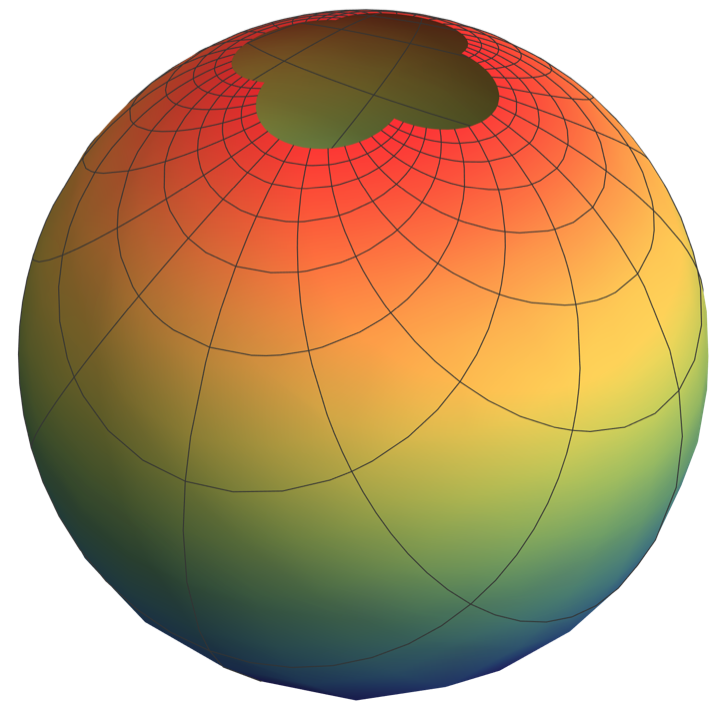
\includegraphics[width=\linewidth]{sup22}
		\end{subfigure}
		\begin{subfigure}{.32\textwidth}
			\centering
			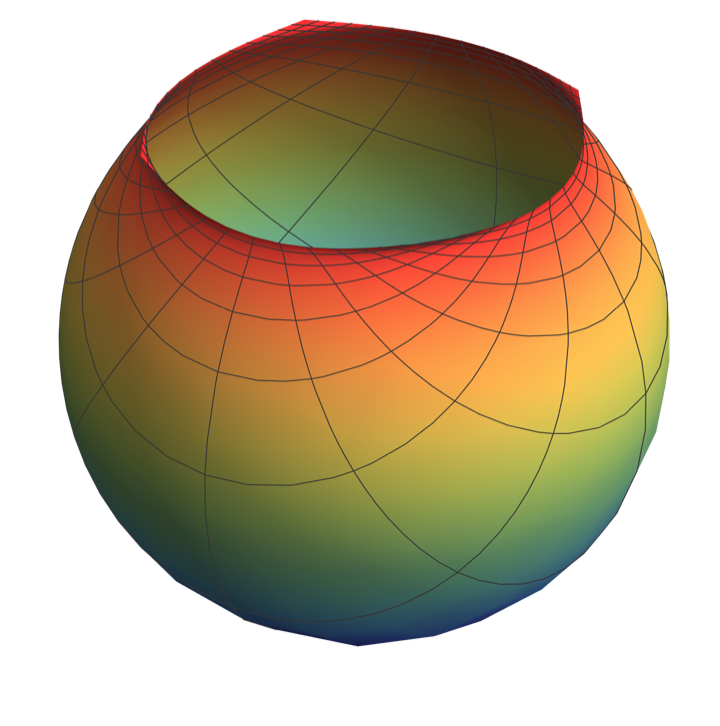
\includegraphics[width=\linewidth]{sup23}
		\end{subfigure}
		\begin{subfigure}{.32\textwidth}
			\centering
			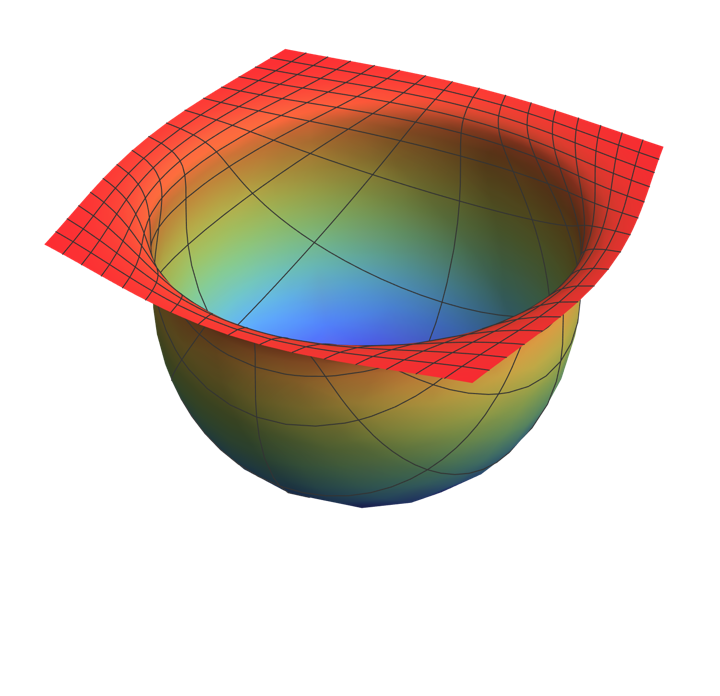
\includegraphics[width=\linewidth]{sup24}
		\end{subfigure}\vspace{.2cm}
		\begin{subfigure}{.25\textwidth}
			\centering
			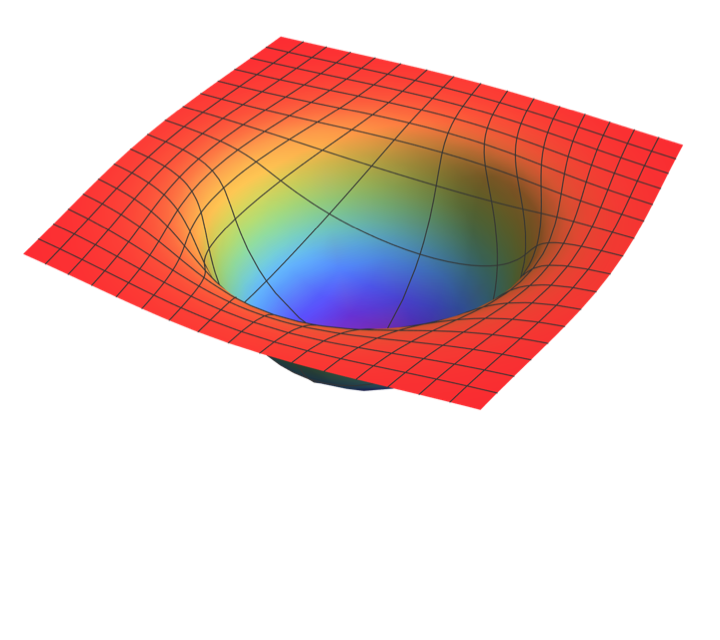
\includegraphics[width=\linewidth]{sup25}
		\end{subfigure}\hspace{-.2cm}
		\begin{subfigure}{0.25\textwidth}
			\centering
			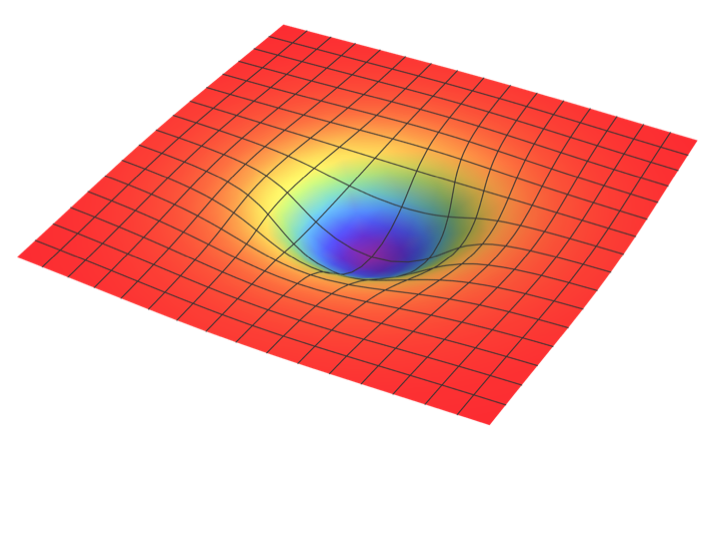
\includegraphics[width=\linewidth]{sup26}
		\end{subfigure}\hspace{-.2cm}
		\begin{subfigure}{0.25\textwidth}
			\centering
			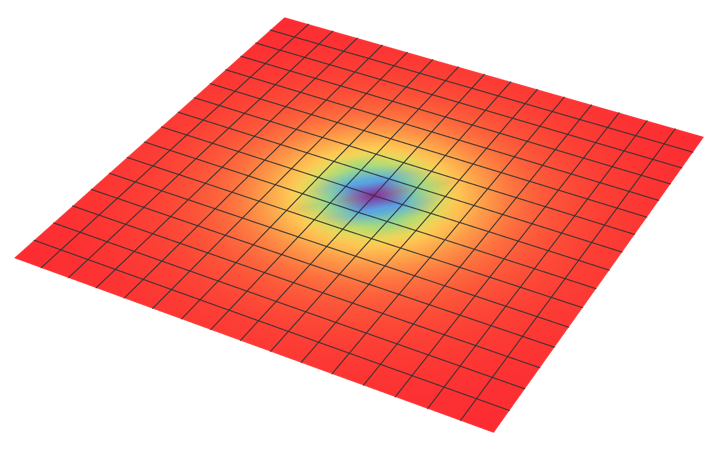
\includegraphics[width=\linewidth]{sup27}
		\end{subfigure}\hspace{-.2cm}
		\begin{subfigure}{0.25\textwidth}
			\centering
			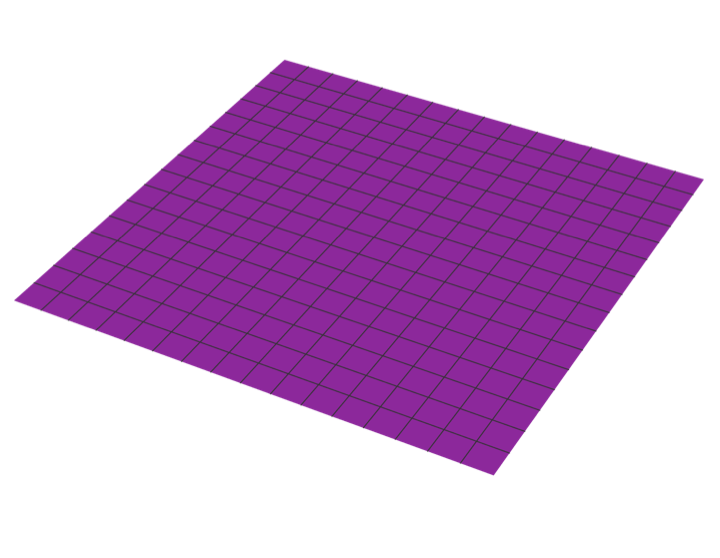
\includegraphics[width=\linewidth]{sup28}
		\end{subfigure}
	\end{figure}
	Notemos en la figura como las rectas coordenadas en el plano se convierten en círculos en la esfera. Aunque cambian sus longitudes, se siguen intersectando en ángulos rectos.
\end{ejem}

\chapter{La aplicación de Gauss}
Según Spivak (ver Spivak, Differential geometry Vol. II), el trabajo más importante en la historia de la geometría diferencial es el artículo de Gauss de 1827 titulado \textit{Disquisitiones generales circa superficies curvas}. Leamos dos párrafos directamente del abstract de este artículo:
\begin{quotation}
	In researches in which an infinity of directions of straight lines in space is concerned, it is advantageous to represent these directions by means of those points upon a fixed sphere, which are the end points of the radii drawn parallel to the lines. The centre and the radius of this auxiliary sphere are here quite arbitrary. The radius may be taken equal to unity. This procedure agrees fundamentally with that which is constantly employed in astronomy, where all directions are referred to a fictitious celestial sphere of infinite radius. Spherical trigonometry and certain other theorems, to which the author has added a new one of frequent application, then serve for the solution of the problems which the comparison of the various directions involved can present.
	
	If we represent the direction of the normal at each point of the curved surface by the corresponding point of the sphere, determined as above indicated, namely, in this way, to every point on the surface, let a point on the sphere correspond; then, generally speaking, to every line on the curved surface will correspond a line on the sphere, and to every part of the former surface will correspond a part of the latter. \textbf{The less this part differs from a plane, the smaller will be the corresponding part on the sphere.} It is, therefore, a very natural idea to use as the measure of the total curvature, which is to be assigned to a part of the curved surface, the area of the corresponding part of the sphere.
\end{quotation}
Así es que la aplicación de Gauss será simplemente la función
\begin{align*}
	N:S&\to S^2\\
	q&\mapsto\frac{\mathbf{x}_u\wedge\mathbf{x}_v}{|\mathbf{x}_u\wedge\mathbf{x}_v|}(q)
\end{align*}
donde $S$ es una superficie regular parametrizada localmente por $u$ y $v$, $S^2$ es la esfera unitaria en $\mathbb{R}^3$ y el símbolo cuña $\wedge$ representa el producto cruz.
\begin{figure}
	\centering
	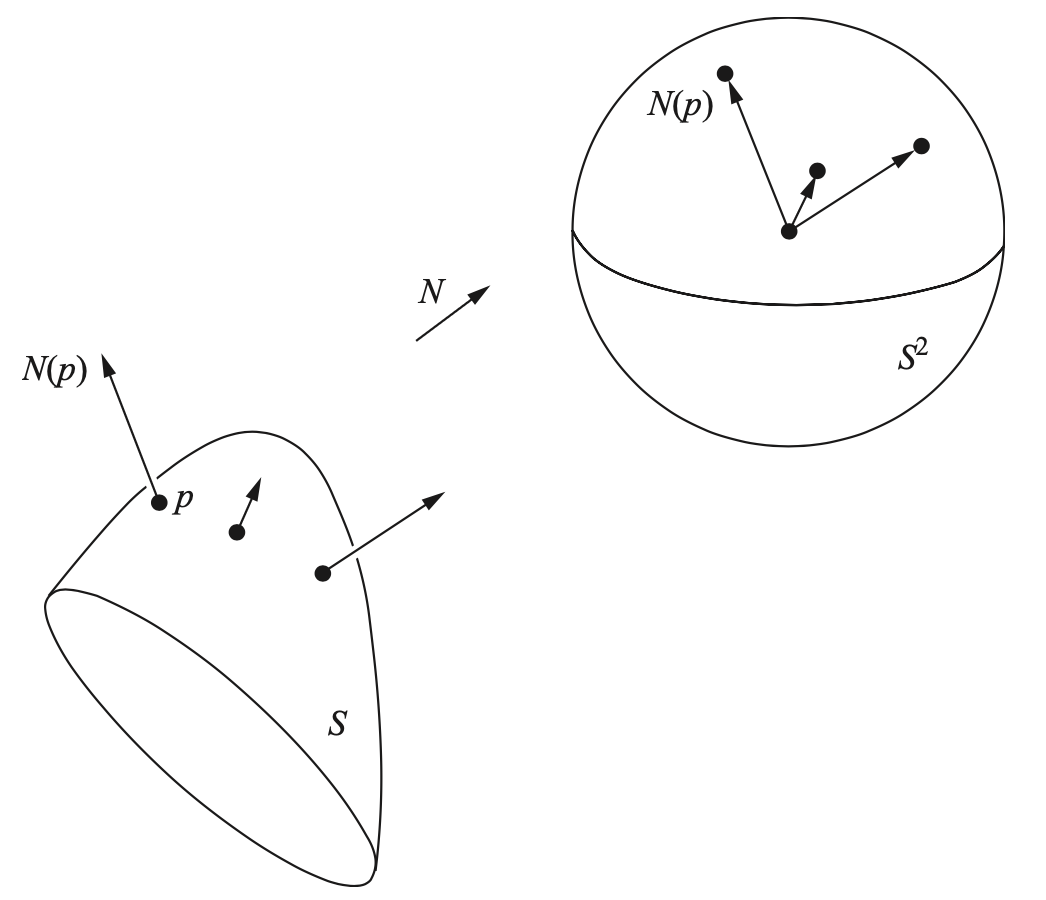
\includegraphics[width=0.7\linewidth]{gauss1}
\end{figure}
Convendrá utilizar superficies orientadas, donde una orientación es simplemente la elección de un campo vectorial normal unitario definido en la superficie.

Ahora de acuerdo a las observaciones de Gauss, para medir qué tanto se curva la superficie tendremos que estudiar qué tanto cambia el vector normal en una parte pequeña de la superficie. Esto sugiere considerar la diferencial de la aplicación de Gauss. Resultará que:
\begin{prop}
	La diferencial $dN_p:T_pS\to T_pS$ es una aplicación lineal autoadjunta, es decir,
	\[\langle dN_p(v),w\rangle=\langle v,dN_p(w)\rangle\]
	para cualesquiera $v,w\in T_pS$.
\end{prop}

Notemos que esta aplicación en efecto está definida de $T_pS$ en sí mismo, pues que el plano tangente a la superficie coincide con el plano tangente a la esfera, pues ambos son planos normales al vector $N(p)$.

Para cualquier aplicación lineal autoadjunta existe una forma bilineal simétrica:
\begin{defn}
	 La forma bilineal simétrica $\mathrm{I\!I}_p(v)=-\langle dN_p(v),v\rangle$ se llama \textbf{segunda forma fundamental}.
\end{defn}
\section{En coordenadas locales}
Supongamos que $M$ es una superficie orinentada en $\mathbb{R}^3$ con una parametrización local $\mathbf{x}:\Omega\subset\mathbb{R}^2\to U\subset M. $ Como antes, pensemos en una curva en la superficie de la forma $\alpha=\mathbf{x}\circ\beta$, donde $\beta$ es una curva en $\Omega$ y la levantamos con la parametrización. Los vectores tangentes a $\alpha$ son de la forma $\alpha'(t)=(u'(t),v'(t))$.

Bueno, si un vector tangente $v\in T_pS$ está expresado en coordenadas locales como $u'\mathbf{x}_u+v'\mathbf{x}_v$, se tiene que
\begin{align*}
	\mathrm{I\!I}_p(v)&=-\langle dN_p(v),v\rangle\\
	&=-\langle dN_p(u'\mathbf{x}_u+v'\mathbf{x}_v),u'\mathbf{x}_u+v'\mathbf{x}_v\rangle\\
	&=-\langle u'dN_p(\mathbf{x}_u),u'\mathbf{x}_u+v'\mathbf{x}_v\rangle-\langle v'dN_p(\mathbf{x}_v),u'\mathbf{x}_u+v'\mathbf{x}_v\rangle\\
	&=-\langle u'dN_p(\mathbf{x}_u),u'\mathbf{x}_u\rangle-\langle u'dN_p(\mathbf{x}_u),v'\mathbf{x}_v\rangle-\langle v'dN_p(\mathbf{x}_v),u'\mathbf{x}_u\rangle-\langle v'dN_p(\mathbf{x}_v),v'\mathbf{x}_v\rangle\\
	&=-(u')^2\langle dN_p(\mathbf{x}_u),\mathbf{x}_u\rangle-u'v'\langle dN_p(\mathbf{x}_u),\mathbf{x}_v\rangle-u'v'\langle dN_p(\mathbf{x}_v),\mathbf{x}_u\rangle-(v')^2\langle dN_p(\mathbf{x}_v),\mathbf{x}_v\rangle\\
	&=-(u')^2\langle dN_p(\mathbf{x}_u),\mathbf{x}_u\rangle-2u'v'\langle dN_p(\mathbf{x}_u),\mathbf{x}_v\rangle-(v')^2\langle dN_p(\mathbf{x}_v),\mathbf{x}_v\rangle\\
	&=-(u')^2e-2u'v'f-(v')^2g\\
\end{align*}


Donde simplemente definimos
\begin{align*}
	e&=-\mathrm{I\!I}_p(\mathbf{x}_u)=-\langle dN_p\mathbf{x}_u,\mathbf{x}_u\rangle=-\langle N_u,\mathbf x_u\rangle\\ 
	f&=-\langle dN_p\mathbf{x}_u,\mathbf{x}_v\rangle=-\langle \mathbf{x}_u,dN_p\mathbf{x}_v\rangle=-\langle\mathbf x_u,N_v\rangle\\ 
	g&=-\mathrm{I\!I}_p(\mathbf{x}_v)=-\langle dN_p\mathbf{x}_v,\mathbf{x}_v\rangle=-\langle N_v,\mathbf x_v\rangle
\end{align*}
Ahora como el vector normal es ortogonal a los dos vectores tangentes básicos, podemos derivar las expresiones $\langle N,\mathbf x_u\rangle=\langle N,\mathbf x_v\rangle=0$ para obtener
\[\langle N_u,\mathbf x\rangle+\langle N,\mathbf x_{uu}\rangle=0\iff\\ e=-\langle N_u,\mathbf x_u\rangle=\langle N,\mathbf x_{uu}\rangle\]
y análogamente
\[f=\langle N,\mathbf x_{uv}\rangle\\
g=\langle N,\mathbf x_{vv}\rangle\]
En fin, la segunda forma fundamental está dada por
\[\mathrm{I\!I}_p(v)=(u')^2e+2u'v'f+(v')^2g\]
Ahora veamos estas cuentas:
\[dN_p=\begin{pmatrix}a_{11}&a_{12}\\a_{21}&a_{22}\end{pmatrix}\]
entonces
\[dN_p(\mathbf{x}_u)=a_{11}\mathbf{x}_u+a_{12}\mathbf{x}_v\qquad\text{y}\qquad dN_p(\mathbf{x}_v)=a_{21}\mathbf{x}_u+a_{22}\mathbf{x}_v\]
Ahora en términos de nuestra matriz $(a_{ij})$,
\begin{align*}
	-e&=\mathrm{I\!I}_p(\mathbf{x}_u)\\
	&=\langle dN_p\mathbf{x}_u,\mathbf{x}_u\rangle\\
	&=\langle a_{11}\mathbf{x}_u+a_{12}\mathbf{x}_v,\mathbf{x}_u\rangle\\
	&=a_{11}\langle\mathbf{x}_u,\mathbf{x}_v\rangle+a_{12}\langle\mathbf{x}_u,\mathbf{x}_v\rangle\\
	&=a_{11}E+a_{12}F\\ \\
	-f&=a_{11}F+a_{21}G=a_{12}E+a_{22}F\\\\
	-g&=a_{12}F+a_{22}G
\end{align*}
Esto se puede expresar como un sistema de ecuaciones:
\[-\begin{pmatrix}e&f\\f & g\end{pmatrix}=\begin{pmatrix}a_{11}&a_{21}\\a_{12}&a_{22}\end{pmatrix}\begin{pmatrix}E&F\\F&G\end{pmatrix}\]
y despejando:
\begin{equation}
	\begin{pmatrix}a_{11}&a_{21}\\a_{12}&a_{22}\end{pmatrix}=-\begin{pmatrix}e&f\\f & g\end{pmatrix}\begin{pmatrix}E&F\\F&G\end{pmatrix}^{-1}
\end{equation}
*¿Por qué la primera forma fundamental es una matriz invertible?*

Como sí lo es, tenemos que 
\[\begin{pmatrix}E&F\\F&G\end{pmatrix}^{-1}=\frac{1}{EG-F^2}\begin{pmatrix}G&-F\\-F&E\end{pmatrix}\]
así que a la mera hora
\[a_{11}=\frac{fF-eG}{EG-F^2},\\
a_{12}=\frac{gF-fG}{EG-F^2},\\
a_{21}=\frac{eF-fE}{EG-F^2},\\
a_{22}=\frac{fF-gE}{EG-F^2}\]
Y lo mejor de todo es que sacando el determinante en $(1)$,
\[K=\det (a_{ij})=\frac{eg-f^2}{EG-F^2}\]
Resulta que también hay una expresión para la curvatura media (no entramos en detalles ahora):
\[H=\frac{1}{2}(\kappa_1+\kappa_2)=-\frac{1}{2}(a_{11}+a_{22})=\frac{1}{2}\frac{eG-2fF+gE}{EG-F^2}\]
Y para las curvaturas principales
\[\kappa=H\pm\sqrt{H^2-K}\]
(No debe haber confusión con el signo pues $\kappa_1\geq\kappa_2$, y la raíz es una cantidad positiva).

\begin{defn}
	La \textbf{curvatura normal} de una curva $C\subset S$  que pasa por un punto $p\in S$ es la magnitud del vector normal a $C$ en $p$, que está dado por $\kappa\mathbf{N}$, cuando lo proyectamos sobre la recta normal a la superficie en $p$.
\end{defn}
\begin{figure}
	\centering
	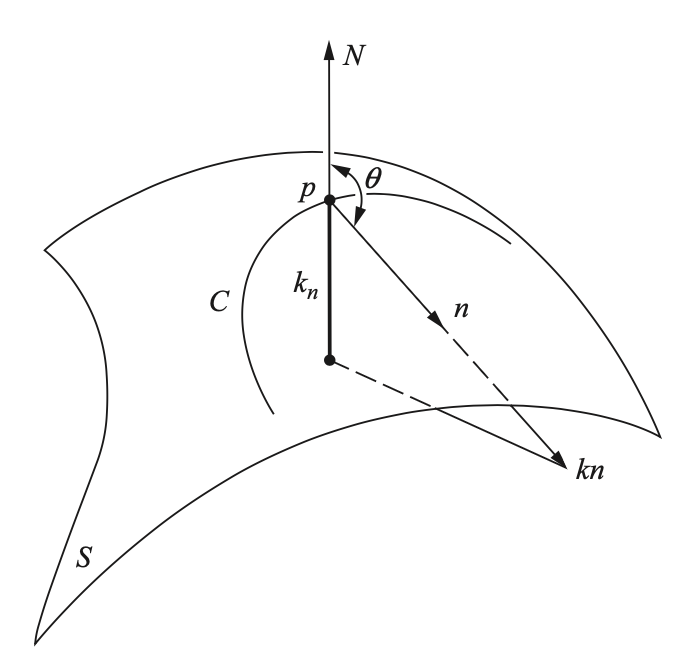
\includegraphics[width=0.5\linewidth]{gauss2}
\end{figure}
Esta cantidad se denotará por $\kappa_\mathbf{N}$. Notemos que como ambos vectores normales son unitarios, el ángulo entre ellos cumple que $\cos\theta=\langle N,\mathbf{{N}}\rangle$, y de hecho la curvatura normal de la curva es tal que $\kappa_\mathbf{{N}}=\kappa\cos\theta$. La curvatura normal cambia de signo si usamos una orientación distinta en nuestra superficie.

De hecho, la segunda forma fundamental nos devuelve este valor cuando la evaluamos en el vector velocidad de una curva parametrizada por longitud de arco, pues en este caso
\[\langle N,\alpha'(s)\rangle=0\implies\langle N(s),\alpha''(s)\rangle=-\langle N'(s),\alpha'(s)\rangle\]
Y luego
\begin{align*}
	\mathrm{I\!I}_p(\alpha'(s))&=-\langle dN_p(\alpha'(0))=\alpha'(0)\rangle\\
	&=-\langle N'(0),\alpha'(0)\rangle\\
	&=\langle N(0),\alpha''(0)\rangle\\
	&=\langle N,\kappa\mathbf{N}\rangle(p)\\
	&=\kappa_\mathbf{N}(p)
\end{align*}
por Frenet-Serret.

Do Carmo incluye en el apéndice el siguiente resultado de álgebra lineal:

Para cualquier aplicación lineal autoadjunta $A:V\to V$ existe una base ortonormal $\{v_1,v_2\}$ de vectores propios. Es decir, $A(v_i)=\lambda_iv_i$ para dos escalares $\lambda_1$ y $\lambda_2$. Expresando a $A$ como una matriz de acuerdo a esta base, resulta ser diagonal. Además, los valores propios son el máximo y el mínimo que alcanza la forma cuadrática $Q(v)=\lambda A(v),v\rangle$ en el círculo unitario de $V$.

Para nuestra aplicación lineal autoadjunta $dN_p$, los valores propios se denotarán por $\kappa_1$ y $\kappa_2$. Surgen algunas definiciones:

\begin{defn}\leavevmode
	\begin{itemize}
		\item El \textbf{máximo} de la curvatura normal $\kappa_1$ y el mínimo de la curvatura normal $\kappa_2$ son llamadas las curvaturas principales en $p$.
		\item Una \textbf{línea de curvatura} es una curva en una superficie tal que para todo punto $p$ la recta tangente a la curva es una dirección principal (es el espacio lineal generado por alguno de los valores propios de $dN_p$.
		\item $\det{dN_p}=\kappa_1\kappa_2:=K$ es la \textbf{curvatura Gaussiana}.
		\item $\frac{1}{2}(\kappa_1+\kappa_2):=H$ es la \textbf{curvatura media}.
		\item Un punto \textbf{umbílico} es donde las dos curvaturas principales son iguales.
	\end{itemize}
\end{defn}
En palabras de Gauss:
\begin{quotation}
	(...) there arises a remarkable relation between this measure of curvature and the curvatures of the curves formed by the intersections of the curved surface with planes normal to it. Euler, as is well known, first showed that two of these cutting planes which intersect each other at right angles have this property, that in one is found the greatest and in the other the smallest radius of curvature; or, more correctly, that in them the two extreme curvatures are found.
\end{quotation}
\begin{ejem}[La silla del macaco]
	La superficie parametrizada por
	\[x=u,\qquad y=v,\qquad z=u^3-3v^2u\]
	es plana en (0,0).
	
	Para verlo, calculemos la segunda forma fundamental y veamos que $K_{(0,0)}=0$.
	\begin{align*}
		\mathbf x_{u}&=(1,0,3u^2-3v^2)\\
		\mathbf x_{v}&=(0,1,-6uv)\\\\
		\mathbf x_{uu}&=(0,0,6u)\\
		\mathbf x_{uv}&=(0,0,-6v)\\
		\mathbf x_{vv}&=(0,0,-6u)\\
	\end{align*}
	Y para encontrar el vector normal recuerdo que si escribimos para una base de $\mathbb R^3$ $\mathbf{i},\mathbf{j},\mathbf{k}$,
	\[\mathbf{a}\times\mathbf{b}=\begin{vmatrix}
		\mathbf{i}&\mathbf{j}&\mathbf{k}\\
		a_1&a_2&a_3\\
		b_1&b_2&b_3
	\end{vmatrix}\]
	Obtenemos que
	\[\mathbf{a}\times\mathbf{b}=\begin{vmatrix}
		a_2&a_3\\
		b_2&b_3
		\end{vmatrix}\mathbf{i}-
		\begin{vmatrix}
		a_1&a_3\\
		b_1&b_3
		\end{vmatrix}\mathbf{j}+
		\begin{vmatrix}
			a_1&a_2\\
			b_1&b_2
		\end{vmatrix}\mathbf{k}\]
	O sea que antes de normalizar,
	\[\mathbf{x}_u\wedge\mathbf{x}_v=(-3u^2+3v^2,6uv,1)\]
	Y luego
	\[|(-3u^2+3v^2,6uv,1)|=\sqrt{(-3u^2+3v^2)^2+36u^2v^2+1}=\sqrt{9(-u^2+v^2)^2+36u^2v^2+1}\]
	De cualquier forma, en el punto $(0,0)$, $N=(0,0,1)$ así que
	\begin{align*}
		e&=\langle N,\mathbf x_{uu}\rangle=\langle(0,0,1),(0,0,6u)\rangle=6u\\
		f&=\langle N,\mathbf x_{uv}\rangle=\langle(0,0,1),(0,0,-6v)\rangle=-6v\\
		g&=\langle N,\mathbf x_{vv}\rangle=\langle(0,0,1),(0,0,-6u)\rangle=-6u
	\end{align*}
	y efectivamente $K=\frac{eg-f^2}{EG-F^2}$ se anula en el origen.
		\begin{figure}[H]
		\centering
		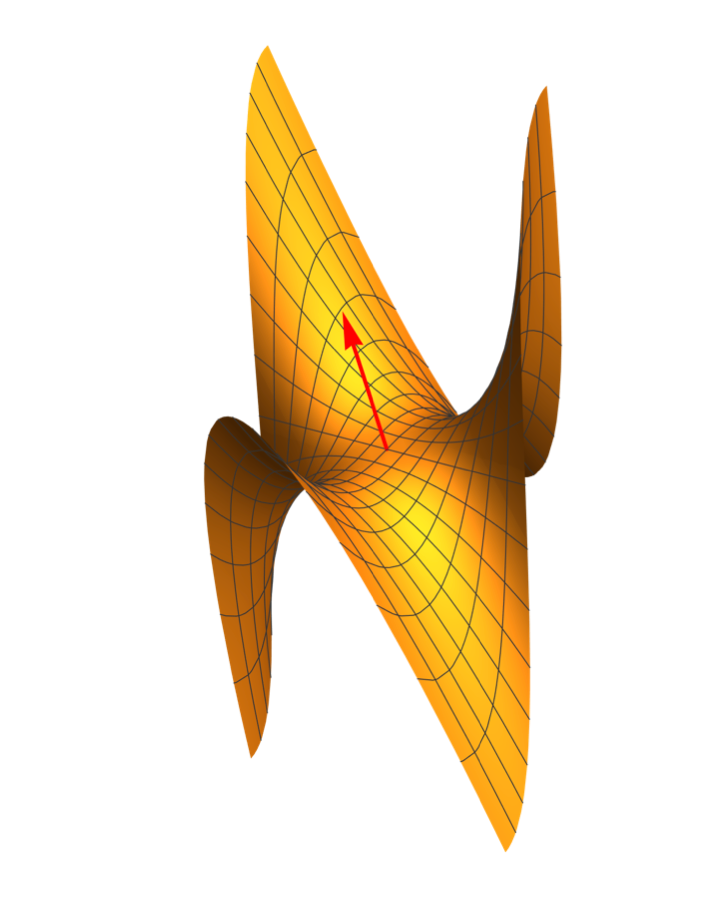
\includegraphics[width=10cm,height=6cm]{gauss3}
	\end{figure}
	\vspace{-0.5cm}
	Notemos que en general, si $\rho=|\langle\mathbf x_u,\mathbf x_v\rangle|$,
	\begin{align*}
		e&=\langle N,\mathbf x_{uu}\rangle=\frac{1}{\rho}\langle(-3u^2+3v^2,6uv,1),(0,0,6u)\rangle=\frac{6u}{\rho}\\
		f&=\langle N,\mathbf x_{uv}\rangle=\frac{1}{\rho}\langle(-3u^2+3v^2,6uv,1),(0,0,-6v)\rangle=\frac{-6v}{\rho}\\
		g&=\langle N,\mathbf x_{vv}\rangle=\frac{1}{\rho}\langle(-3u^2+3v^2,6uv,1),(0,0,-6u)\rangle=\frac{-6u}{\rho}
	\end{align*}
	Así que de hecho
	\[K=\frac{eg-f^2}{EG-F^2}=\frac{-36u-36v}{\rho^2(EG-F^2)}\]
	Pero fijémonos que siempre es cierto que
	\[\Vert\mathbf{a}\times\mathbf{b}\Vert^2=\begin{vmatrix}
		\mathbf{a}\cdot\mathbf{a}&\mathbf{a}\cdot\mathbf{b}\\
		\mathbf{a}\cdot\mathbf{b}&\mathbf{b}\cdot\mathbf{b}\end{vmatrix}=\Vert\mathbf{a}\Vert^2\Vert\mathbf{b}\Vert^2-(\mathbf{a}\cdot\mathbf{b})^2\]
	Así que en realidad $\rho=|\mathbf x_u\wedge \mathbf x_v|=\sqrt{EG-F^2}$, y el denominador se vuelve simplemente $(EG-F^2)^2$, un número que siempre es positivo. Por lo tanto, la silla del macaco tiene curvatura negativa salvo en el origen, donde es plana.
\end{ejem}

\section{El teorema de Gauus}
\subsection{Los símbolos de Christoffel}
Notando que los tres vectores $\mathbf x_u,\mathbf x_v$ y $N$ son una base de $\mathbb R^3$, deben existir los coeficientes que hagan ciertas las siguientes ecuaciones para las derivadas:
\begin{align*}
	\mathbf x_{uu}=\Gamma^1_{11}\mathbf x_u+\Gamma^2_{11}\mathbf x_v+L_1N\\
	\mathbf x_{uv}=\Gamma^1_{12}\mathbf x_u+\Gamma^2_{12}\mathbf x_v+L_2N\\
	\mathbf x_{vu}=\Gamma^1_{21}\mathbf x_u+\Gamma^2_{21}\mathbf x_v+\bar L_2N\\
	\mathbf x_{vv}=\Gamma^1_{22}\mathbf x_u+\Gamma^2_{22}\mathbf x_v+L_3N\\
	N_u=a_{11}\mathbf x_u+a_{21}\mathbf x_v\\
	N_u=a_{12}\mathbf x_u+a_{22}\mathbf x_v
\end{align*}
donde las últimas dos ecuaciones responden a la notación de la sección anterior:
\[dN_p=\begin{pmatrix}a_{11}&a_{12}\\a_{21}&a_{22}\end{pmatrix}\]
de forma que
\[dN_p(\mathbf{x}_u)=a_{11}\mathbf{x}_u+a_{12}\mathbf{x}_v\qquad\text{y}\qquad dN_p(\mathbf{x}_v)=a_{21}\mathbf{x}_u+a_{22}\mathbf{x}_v\]
y simplemente recordando que la derivada direccional en la dirección de cualquier vector es la derivada de la función evaluada en ese vector, se obtienen los últimos dos renglones. Ya sabemos los valores de estos coeficientes en términos de la primera y segunda formas fundamentales.

Haciendo productos internos de las primeras cuatro ecuaciones de arriba con el vector $N$, obtenemos que 
\[L_1=e,\qquad L_2=\bar L_2=f,\qquad L_3=g\]
Y que los "símbolos de Christoffel" $\Gamma^k_{ij}$ están dados en términos únicamente de la primera forma fundamental y sus derivadas. Específicamente:
\begin{align*}
	\Gamma^1_{11}E+\Gamma^2_{11}F&=\langle \mathbf x_{uu},\mathbf x_u\rangle=\frac{1}{2}E_u\\
	\Gamma^1_{11}F+\Gamma^2_{11}G&=\langle \mathbf x_{uu},\mathbf x_v\rangle=F_u+\frac{1}{2}E_v\\\\
	\Gamma^1_{12}E+\Gamma^2_{12}F&=\langle \mathbf x_{uv},\mathbf x_v\rangle=\frac{1}{2}E_v\\
	\Gamma^1_{1}F+\Gamma^2_{12}G&=\langle \mathbf x_{u},\mathbf x_v\rangle=\frac{1}{2}G_u\\ \\
	\Gamma^1_{22}E+\Gamma^2_{22}F&=\langle \mathbf x_{vv},\mathbf x_u\rangle=F_v+\frac{1}{2}G_u\\
	\Gamma^1_{22}F+\Gamma^2_{22}G&=\langle \mathbf x_{vv},\mathbf x_v\rangle=\frac{1}{2}G_v
\end{align*}
Ahora resolviendo este sistema por pares (no es difícil, quizá valga la pena checar uno) se obtienen las ecuaciones:
\[\begin{split}
	\Gamma^1_{11}&=\frac{GE_u-2FF_u+FE_v}{2(EG-F^2)}\\
	\Gamma^1_{12}&=\frac{GE_v-FG_u}{2(EG-F^2)}\\
	\Gamma^2_{11}&=\frac{2GF_v-GG_u-FG_v}{2(EG-F^2)}
\end{split}
\begin{split}
	\qquad\qquad\Gamma^2_{11}&=\frac{2EF_u-EE_v+FE_u}{2(EG-F^2)}\\
	\qquad\qquad \Gamma^2_{12}&=\frac{EG_u-FE_v}{2(EG-F^2)}\\
	\qquad\qquad\Gamma^2_{22}&=\frac{EG_v-2FF_v+FG_u}{2(EG-F^2)}
\end{split}\]
Ahora sí, lo más importante es que
\begin{quote}
	Cualquier concepto geométrico expresado en términos de los símbolos de Christoffel es invariante bajo isometrías.
\end{quote}
Y más aún, se demuestra la igualdad
\[(\Gamma^2_{12})_u+(\Gamma^2_{11})_v+\Gamma^1_{12}\Gamma^2_{11}+\Gamma^2_{12}\Gamma^2_{12}-\Gamma^2_{11}\Gamma^2_{22}-\Gamma^1_{1}\Gamma^2_{12}=-EK\]
Así es que 

\begin{teo}[Teorema Egregium] La curvatura Gaussiana es invariante bajo isometrías locales.
\end{teo}
En palabras de Gauss:
\begin{quotation}
	Therefore we notice that, in order to determine the measure of curvature, it is necessary to know only the general expression for a linear element; the expressions for the coordinates x, y, z are not required. A direct result from this is the remarkable theorem: If a curved surface, or a part of it, can be developed upon another surface, the measure of curvature at every point remains unchanged after the development.
\end{quotation}
Donde la primera forma fundamental se esconde tras el concepto de "linear element" que de hecho no es desconocido para nosotros: se trata de la expresión $\sqrt{E(u')^2+2Fu'v'+G(v')^2}$. ¿Y qué consecuencias tiene esto? Continuamos citando el abstract:
\begin{quotation}
	(...) we see that two essentially different relations must be distinguished, namely, on the one hand, those that presuppose a definite form of the surface in space; on the other hand, those that are independent of the various forms which the surface may assume.
\end{quotation}
Y tenemos dos teoremas que son consecuencia:
\begin{quotation}
	If upon a curved surface a system of infinitely many shortest lines of equal lengths be drawn from one initial point, then will the line going through the end points of these shortest lines cut each of them at right angles.
	
	If at every point of an arbitrary line on a curved surface shortest lines of equal lengths be drawn at right angles to this line, then will all these shortest lines be perpendicular also to the line which joins their other end points.
\end{quotation}
Y no podemos irnos sin agregar que:
\begin{quotation}
	The excess of the sum of the angles of a triangle formed by shortest lines over two right angles is equal to the total curvature of the triangle.
\end{quotation}
Por ahora no ahondaremos en estas afirmaciones.
\begin{ejem}[Helicoide y cuerno: el recíproco del teorema de Gauss]
	Mostraremos que estas dos superficies tienen misma curvatura Gaussiana pero no son localmente isométricas.
	
	Primero tomemos la helicoide
	\[{\mathbf{x}}({u},{v})= (u\cos{v},u\sin v,v)\]
	Y calculamos que:
	\begin{align*}
		\mathbf x_u&=(\cos v,\sin v,0)\\
		\mathbf x_v&=(-u\sin v,u\cos v,1)\\\\
		E&=1\\
		F&=0\\
		G&=u^2+1\\\\
		\mathbf x_{uu}&=(0,0,0)\\
		\mathbf x_{uv}&=(-\sin v,\cos v,0)\\
		\mathbf x_{vv}&=(-u\cos v,-u\sin v,0)\\
		N&=\frac{1}{\sqrt{u^2+1}}(\sin v,-\cos v,u)\\\\
		e&=0\\
		f&=-\frac{1}{\sqrt{u^2+1}}\\
		g&=0\\\\
		K&=\frac{-\frac{1}{u^2+1}}{{u^2+1}}=-\frac{1}{(u^2+1)^2}
	\end{align*}
	Ahora el cuerno
	\[\bar{\mathbf{x}}(\bar{u},\bar{v})= ( \bar u\cos{ \bar v}, \bar u\sin  \bar v,\log \bar u)\]
	Y luego:
	\begin{align*}
		\bar{\mathbf x}_{\bar{u}}&=(\cos \bar v,\sin\bar v,\frac{1}{\bar u})\\
		\bar{\mathbf x}_{\bar{v}}&=(-\bar u\sin\bar v,\bar u\cos \bar v,0)\\\\
		\bar E&=1+\frac{1}{\bar{u}^2}\\
		\bar F&=0\\
		\bar G&=\bar u^2\\\
		...\\
		\bar K&=-\frac{1}{(\bar{u}^2+1)^2}
	\end{align*}
	Recordando nuestra \hyperref[prop:reciproca]{herramienta de isometrías}, concluimos que la función $\varphi=\bar{\mathbf{x}}\circ\mathbf x^{-1}$ no es una isometría.
	
	Pero, ¿que no podrían existir otras parametrizaciones que hicieran estas superficies isométricas? Notando que la curvatura Gaussiana no depende de la parametrización (pues es el determinante de la diferencial del vector normal unitario), como tenemos que $K=\bar{K}$, entonces
	\[(u^2+1)^2=(\bar u^2+1)^2\iff u^2=\bar u^2\iff  u=\pm\bar u\]
	Ahora cambiando cualquier parametrización sin alterar esta relación **¡¡Falta!!**
	\begin{figure}[H]
		\centering
		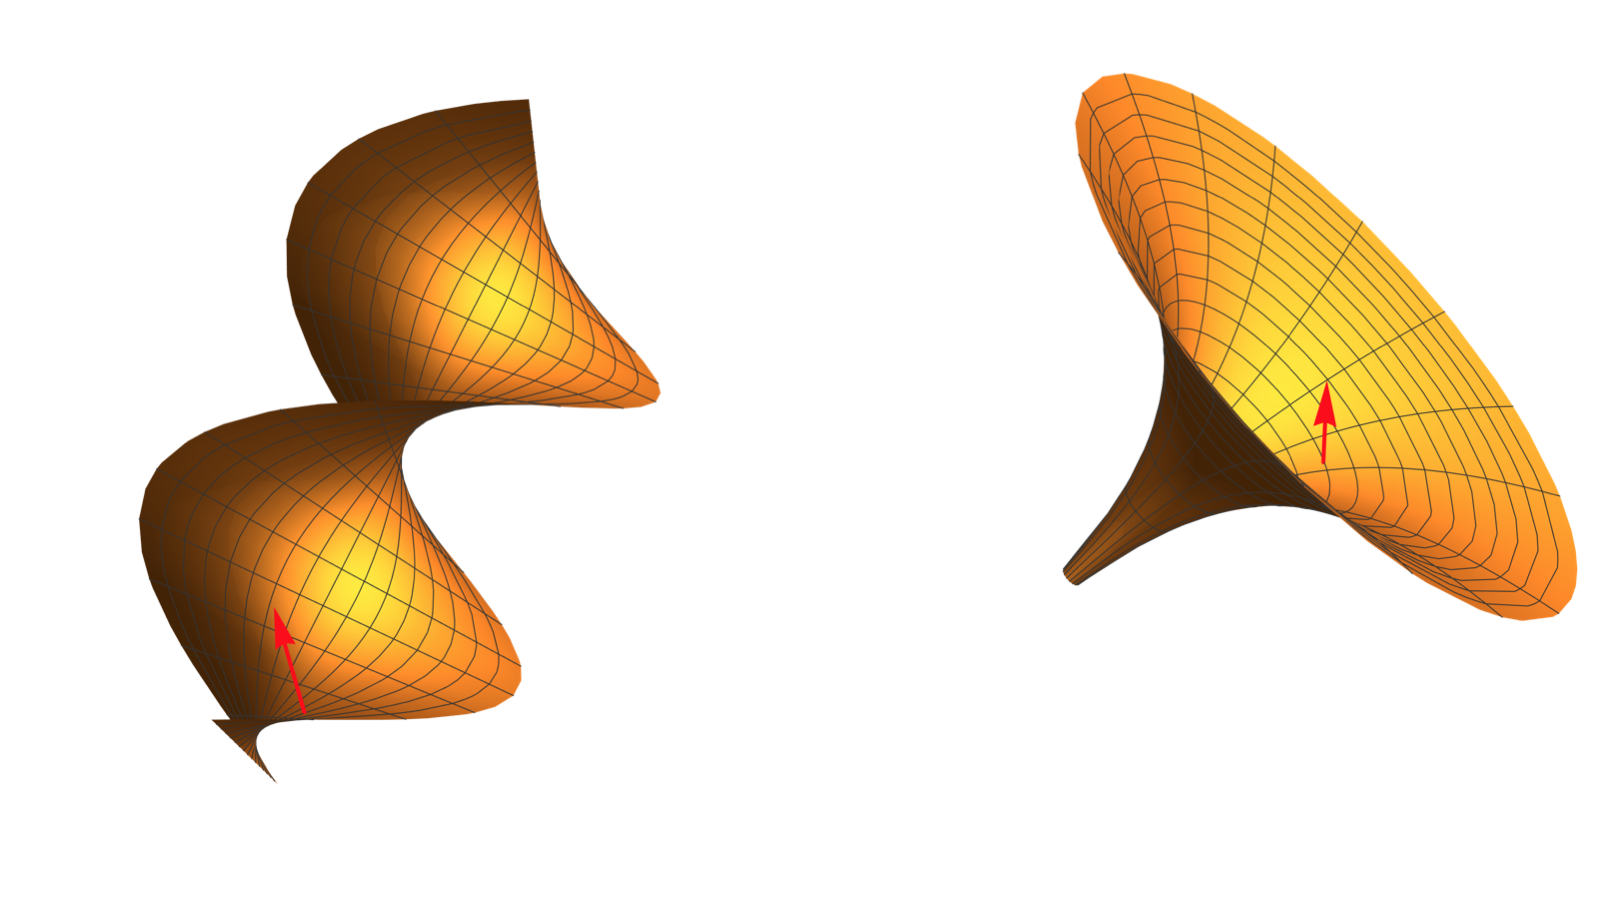
\includegraphics[width=\linewidth]{gauss4}
	\end{figure}
	\vspace{-1cm}
\end{ejem}
\begin{pregunta}
	¿No podrían existir otras parametrizaciones que hicieran estas superficies isométricas? ¿La curvatura Gaussiana depende de la parametrización?
\end{pregunta}

\subsection{Los símbolos de Christoffel de una superficie de revolución}
\begin{ejem}[Ejemplo 1, Sección 4.3, Do Carmo]
	Simplemente escribiremos aquí que para un superficie de revolución parametrizada por
	\[\mathbf x(u,v)=(f(v)\cos u,f(v)\sin u,g(v)),\qquad f(v)\neq0\]
	se tiene que
	\[E=(f(v))^2,\qquad F=0\qquad G=(f'(v))^2+(g'(v))^2\]
	y que
	\begin{align*}
		\Gamma^1_{11}=0,\qquad\Gamma^2_{11}=-\frac{ff'}{(f')^2+(g')^2}\\
		\Gamma^1_{12}=\frac{ff'}{f^2},\qquad\Gamma^2_{12}=0\\
		\Gamma^1_{22}=0,\qquad\Gamma^2_{22}=\frac{f'f''+g'g''}{(f')^2+(g')^2}
	\end{align*}
\end{ejem}
\begin{ejer}[Los símbolos de Christoffel de la helicoide]
	Ya hemos hecho bastante trabajo con la helicoide. Para calcular los símbolos de Christoffel debemos usar las seis fórmulas de la sección anterior y la primera fórmula fundamental de la helicoide, que ya calculamos:
	\begin{align*}
	\begin{matrix}
		\Gamma^1_{11}E+\Gamma^2_{11}F&=\langle \mathbf x_{uu},\mathbf x_u\rangle=\frac{1}{2}E_u&&&&&E=1\\
		\Gamma^1_{11}F+\Gamma^2_{11}G&=\langle \mathbf x_{uu},\mathbf x_v\rangle=F_u+\frac{1}{2}E_v&&&&&F=0\\&&&&&&G=u^2+1\\
		\Gamma^1_{12}E+\Gamma^2_{12}F&=\langle \mathbf x_{uv},\mathbf x_v\rangle=\frac{1}{2}E_v\\
		\Gamma^1_{1}F+\Gamma^2_{12}G&=\langle \mathbf x_{u},\mathbf x_v\rangle=\frac{1}{2}G_u\\ \\
		\Gamma^1_{22}E+\Gamma^2_{22}F&=\langle \mathbf x_{vv},\mathbf x_u\rangle=F_v+\frac{1}{2}G_u\\
		\Gamma^1_{22}F+\Gamma^2_{22}G&=\langle \mathbf x_{vv},\mathbf x_v\rangle=\frac{1}{2}G_v
	\end{matrix}
	\end{align*}
	Sustituyendo:
	\begin{align*}
		\Gamma^1_{11}&=\langle \mathbf x_{uu},\mathbf x_u\rangle=\frac{1}{2}E_u=0\\
		\Gamma^2_{11}(u^2+1)&=\langle \mathbf x_{uu},\mathbf x_v\rangle=F_u+\frac{1}{2}E_v=0\implies \Gamma^2_{11}=0\\\\
		\Gamma^1_{12}&=\langle \mathbf x_{uv},\mathbf x_v\rangle=\frac{1}{2}E_v=0\\
		\Gamma^2_{12}(u^2+1)&=\langle \mathbf x_{u},\mathbf x_v\rangle=\frac{1}{2}G_u=\frac{1}{2}2u=u\implies\Gamma^2_{12}=\frac{u}{u^2+1}\\ \\
		\Gamma^1_{22}&=\langle \mathbf x_{vv},\mathbf x_u\rangle=\frac{1}{2}G_u=u\\
		\Gamma^2_{22}G&=\langle \mathbf x_{vv},\mathbf x_v\rangle=\frac{1}{2}G_v=0
	\end{align*}
	Ahora recordemos que la helicoide es localmente isométrica a la catenoide. Pero parece que estos símbolos de Christoffel no pueden ser los de la catenoide cuando usamos las fórmulas para superficies de revolución. ¿Qué está pasando? ¿Es posible hacer que coincidan los símbolos de Christoffel de las dos superficies?
	\begin{figure}[H]
		\centering
		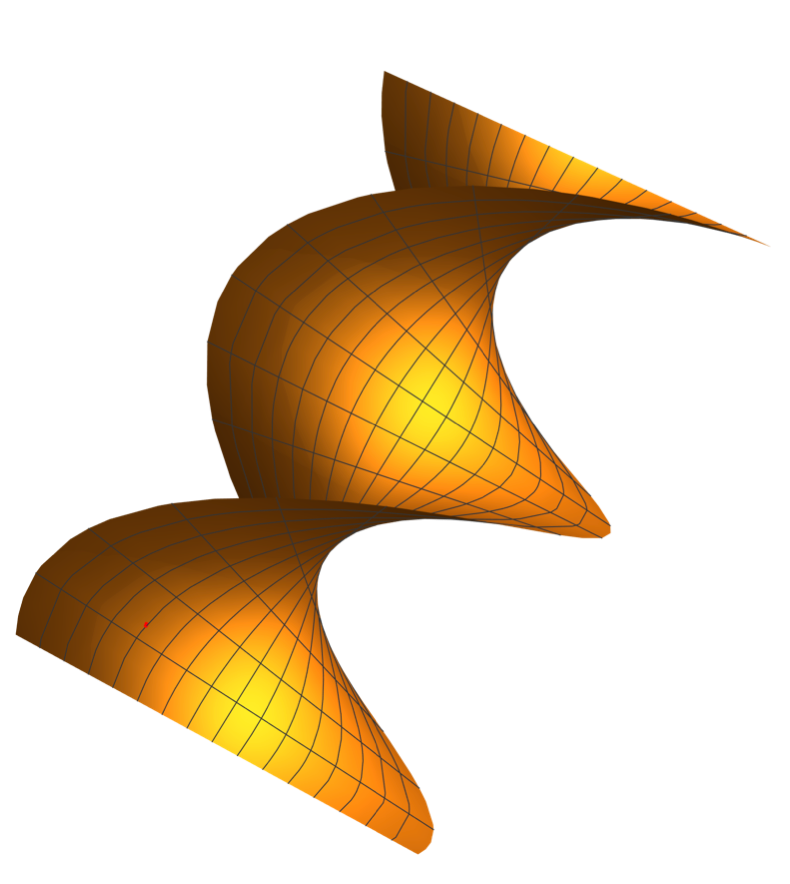
\includegraphics[width=0.4\linewidth]{gauss5}
	\end{figure}
\end{ejer}

\section{Campos vectoriales y geodésicas}
\subsection{Campos vectoriales paralelos}
Primero necesitamos algunas definiciones:
\begin{defn}\leavevmode
	\begin{itemize}
		\item Un \textbf{campo vectorial} en un abierto $U\subseteq S$ es una función $w$ que a cada punto le asocia un vector $w(p)\in T_pS$.
		\item Un \textbf{campo vectorial es diferenciable} en $p$ si existe alguna parametrización $\mathbf x(u,v)$ alrededor de $p$ tal que las funciones componentes $a$ y $b$ en la expresión $w(p)=a\mathbf x_u+b\mathbf x_v$ son funciones diferenciables en $p$. Un campo vectorial es diferenciable si es diferenciable en todos los puntos.
		\item Sea $w$ un campo vectorial diferenciable en algún abierto $U\subseteq S$ y $p$ algún punto en $U$. Tomemos un vector $y\in T_pS$ y una curva $\alpha$ que realice este vector en el sentido de que $\alpha(0)=p$ y $\alpha'(0)=y$.    Podemos considerar la restricción de $w$ a la curva $\alpha$, y de hecho podemos derivarlo como función de $\mathbb R$ en $\mathbb R^3$ para obtener el vector $(dw/dt)(0)$. Aunque éste no tiene por qué ser un vector en $T_pS$, podemos considerar su proyección en el plano tangente, que definiremos como la \textbf{derivada covariante} de $w$ en $p$ respecto a $y$, denotada por $\frac{Dw}{dt}$.
	\end{itemize}
\end{defn}
\begin{figure}
	\centering
	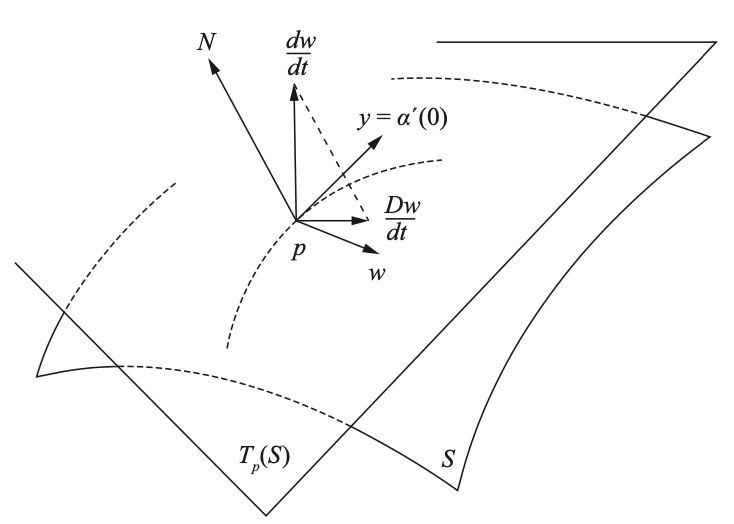
\includegraphics[width=0.5\linewidth]{gauss6}
\end{figure}
Lo primero que debemos demostrar es que la derivada covariante es un concepto intrínseco a la superficie. Esto no es obvio, ya que se definió usando el espacio ambiente $\mathbb R^3$. Por las observaciones de la sección anterior, basta demostrar que la derivada covariante tiene una expresión en términos de los símbolos de Christoffel.

Supongamos que nuestra curva está dada por $\alpha(t)=\mathbf x(u(t),v(t))$. Al restringir nuestro campo vectorial a la curva, como arriba, obtenemos la expresión $w(p)=a\mathbf x_u+b\mathbf x_v$. En este caso, $a$ y $b$ son funciones de $\mathbb R $ en $\mathbb R$, mientras que los vectores básicos están dados por la composición $\mathbf x_u(u(t),v(t))$. La derivada respecto a $t$ de esta última expresión es
\[\frac{d}{dt}\mathbf x_u(u(t),v(t))=(\mathbf x_{uu},\mathbf x_{uv})·(u'(t),v'(t))=\mathbf u'(t)\mathbf x_{uu}+v'(t)\mathbf x_{uv}\]
evaluando los vectores de segunda derivada parcial en el punto $(u(t),v(t))$.

En fin, la derivada del campo respecto a $t$ es:
\begin{align*}
	\frac{dw}{dt}&=\frac{d}{dt}a\mathbf x_u+b\mathbf x_v\\
	&=\frac{d}{dt}\Big(a(t)\mathbf x_u(u(t),v(t))+b(t)\mathbf x_v(u(t),v(t))\Big)\\
	&=a'(t)\mathbf x_u+a(t)\frac{d}{dt}\mathbf x_u(u(t),v(t))+b'(t)\mathbf x_v+b(t)\frac{d}{dt}\mathbf x_v(u(t),v(t))\\
	&=a'(t)\mathbf x_u+a(t)\big(u'(t)\mathbf x_{uu}+v'(t)\mathbf x_{uv}\big)
	+b'(t)\mathbf x_v+b(t)\big(u'(t)\mathbf x_{vu}+v'(t)\mathbf x_{vv}\big)\\
\end{align*}
Simplificando la notación,
\[\frac{dw}{dt}=a(u'\mathbf x_{uu}+v'\mathbf x_{uv})+b(u'\mathbf x_{uv}+v'\mathbf x_{vv})+a'\mathbf x_u+b'\mathbf x_v\]
Una vez aclarado esto, recordemos las expresiones de la sección anterior para las segundas derivadas parcial, que de hecho fue cuando definimos los símbolos de Christoffel. Para obtener la derivada covariante basta tomar las componentes en el plano tangente y ignorar la tercera, que correspondía al vector normal.

Sustituyendo, de acuerdo a Do Carmo, obtenemos
\begin{equation}
	\begin{aligned}
		\frac{Dw}{dt}&=(a'+\Gamma^1_{11}au'+\Gamma^1_{12}av'+\Gamma^1_{12}bu'+\Gamma^1_{22}bv')\mathbf x_u\\
		&+(b'+\Gamma^2_{11}au'+\Gamma^2_{12}av'+\Gamma^2_{12}bu'+\Gamma^2_{22}bv')\mathbf x_v
	\end{aligned}
\end{equation}
En fin, la derivada covariante tiene una expresión en términos de los símbolos de Christoffel así que, como la curvatura Gaussiana, es una propiedad intrínseca de la superficie: sólo depende de la primera forma fundamental. Notemos además que la curva $\alpha$ tampoco juega un papel importante: sólo es relevante el vector tangente con el que empezamos $y=(u',v')$.
\begin{obs}
	Cuando decimos que una propiedad es "intrínseca a una superficie", nos referimos a que está determinada únicamente por la primera forma fundamantal, y por lo tanto es invariante bajo isometrías. Otro significado importante, y es lo que hemos comentado aquí, es que "no depende del espacio ambiente". Claro, como la propiedad sólo depende de la primera forma fundamental, está dado en términos de las derivadas de la parametrización local, y de hecho no necesitamos hacer uso del vector normal en $\mathbb R^3$. Aunque claro, es mucho más didáctivo usar el espacio ambiente para definir la derivada covariante…
\end{obs}
Introducimos algunas definiciones más:
\begin{defn}\leavevmode
	\begin{itemize}
		\item Un campo vectorial a lo largo de una curva $w$ es una asociación que a cada punto del dominio de una curva $\alpha:I\to S$ le asocia un vector en el plano tangente. El campo es diferenciable si existe alguna parametrización para la cual las funciones componentes en la expresión $w(t)=a\mathbf x_u+b\mathbf x_v$ son diferenciables.
		\item La derivada covariante de un campo vectorial diferenciable a lo largo de una curva está dado por la expresión $(2)$.
		\item Un campo vectorial $w$ a lo largo de una curva $\alpha:I\to S$ es \textbf{paralelo} si $\frac{Dw}{dt}=0$ para toda $t\in I$. Siguiendo a Petrunin (ver Petrunin, What is differential geometry?): un campo vectorial a lo largo de una curva es paralelo si la derivada del campo es ortogonal al plano tangente.
	\end{itemize}
\end{defn}

Pensemos en un campo vectorial paralelo en $\mathbb R^3$. Se trata de una colección de vectores que apuntan en la misma dirección (de hecho, si pensamos que los vectores están anclados en el origen, no es más que un campo vectorial constante). Esto nos hace pensar que nuestro campo debe satisfacer que $w'=0$. Ahora, si el campo vectorial es tangente a alguna superficie, de igual forma quisiéramos que tuviera derivada cero para decir que es paralelo, pero esto en general no es posible si la superficie es curva.

Los planos tangentes a una superficie curva van cambiando conforme nos desplazamos en la superficie, y así, un campo vectorial tangente a la superficie no puede ser constante, es decir no puede ser realmente paralelo. Entonces, la derivada no puede ser cero.

Lo que sí podemos hacer con la derivada es comparar la derivada con el plano tangente. Nos gustaría que esta derivada fuera lo más cercano a cero, esto es, que cambiara sólo lo mínimo posible dado el cambio en el plano tangente: queremos que la derivada se mueva junto con el plano tangente. Esa propiedad quiere decir que la derivada sea siempre perpendicular al plano tangente, luego, la proyección de la derivada al plano tangente es el cero, es decir, $\frac{Dw}{dt}=0$.
\begin{prop}
	Si $v$ y $w$ son dos campos paralelos a lo largo de una curva $\alpha:I\to S$, entonces $\langle v(t),w(t)\rangle$ es constante. En particular $|v(t)|$ y $|w(t)|$ son constante y el ángulo entre $v(t)$ y $w(t)$ también.
\end{prop}
\begin{proof}
	Como la derivada de los campos es ortogonal al plano tangente, $\langle v(t),w'(t)\rangle=0=\langle v'(t),w(t)\rangle$. Luego $\langle v(t),w(t)\rangle'=\langle v'(t),w(t)\rangle+\langle v(t),w'(t)\rangle=0.$
\end{proof}
\subsection{Extra: dos fórmulas de geometría Riemanniana}
Damos un vistazo a la geometría diferencial en variedades de dimensión arbitraria.

Mostramos primero una fórmula para los símbolos de Christoffel:
\[\Gamma^k_{ij}=\frac{1}{2}\sum_m g^{km}\Big(\frac{\partial g_{jm}}{\partial x^i}+\frac{\partial g_{im}}{\partial x^j}-\frac{\partial g_{ij}}{\partial x^m}\Big)\]
donde $g_{ij}$ son coeficientes del tensor métrico, es decir, el producto interno de los vectores tangentes básicos con índices $i$ y $j$. Y bueno, $g^{ij}$ es la matriz inversa.

Y luego una fórmula (de hecho así se definen los símbolos de Christoffel) para la derivada covariante del campo vectorial $\mathbf x_j$ respecto al campo vectorial $\mathbf x_i$:
\[\nabla_{\mathbf x_i}\mathbf x_j=\sum_{k}\Gamma^k_{ij}\mathbf x_k\]
Notemos que esta derivada covariante está dada para campos vectoriales definidos en conjuntos abiertos y no sobre curvas. Desde luego, hay una relación entre ambos conceptos.

\section{Transporte paralelo}
\begin{prop}
	Sean $\alpha:I\to S$ una curva parametrizada en $S$ y $w_0\in T_{\alpha(t_0)}S$  para algún $t_0\in I$. Entonces, existe un único campo paralelo $w$ a lo largo de $\alpha$ tal que $w(t_0)=w_0$.
\end{prop}
\begin{proof}
	Usamos el teorema de existencia y unicidad de ecuaciones diferenciales: necesitamos encontrar un campo vectorial para el cual se satisfaga $(2)$ y la condición incial $w(t_0)=w_0$.
\end{proof}
Esta proposición nos permite definir:
\begin{defn}
	Sean $\alpha:I\to S$ una curva parametrizada en $S$ y $w_0\in T_{\alpha(t_0)}S$  para algún $t_0\in I$. Luego, sea $w$ el un único campo paralelo a lo largo de $\alpha$ tal que $w(t_0)=w_0$. El vector $w(t_1)$ es el **transporte paralelo** de $w_0$ a lo largo de $\alpha$ en $t_1$.
\end{defn}
\begin{obs}
	\begin{enumerate}\leavevmode
		\item Si la curva es regular, el transporte paralelo no depende de la parametrización de la curva. Esto es, un campo vectorial paralelo sigue siendo paralelo cuando hacemos un cambio de parametrización.
		\item El transporte paralelo es una isometría lineal. Dados dos puntos $p$ y $q$ en una superficie y una curva $\alpha:[a,b]\to S$ que los une en sus extremos, tenemos la función $P_\alpha:T_pS\to T_qS$ que a cualquier vector tangente a la superficie en $p$ le asocia su transporte paralelo a lo largo de $\alpha$ en $q$.
		\item Como la derivada covariante es la proyección de la derivada usual del campo sobre el plano tangente, se sigue que si dos superficies "son tangentes" a lo largo de una curva (esto es, el plano tangente es el mismo para todos los puntos de la curva), entonces las derivadas covariantes de cualquier campo definido a lo largo de la curva coinciden en ambas superficies. Luego, el transporte paralelo de algún vector $w_0$ es el mismo para ambas superficies.
	\end{enumerate}
\end{obs}
\begin{ejem}[transporte paralelo en la esfera. Ejemplo 1, Sección 4.4, Do Carmo.]
	Consideremos un paralelo $C$ de colatitud $\varphi$ (ver figura) en la esfera unitaria orientada, y un vector $w_0$ tangente unitario a $C$ en algún punto $p$. Determinaremos el transporte paralelo de $w_0$ a lo largo de $C$ cuando está parametrizado por longitud de arco con parámetro $s$ y en $s=0$ tenemos el punto $p$.
	
	Observemos la siguiente figura:
	\begin{figure}[H]
		\centering
		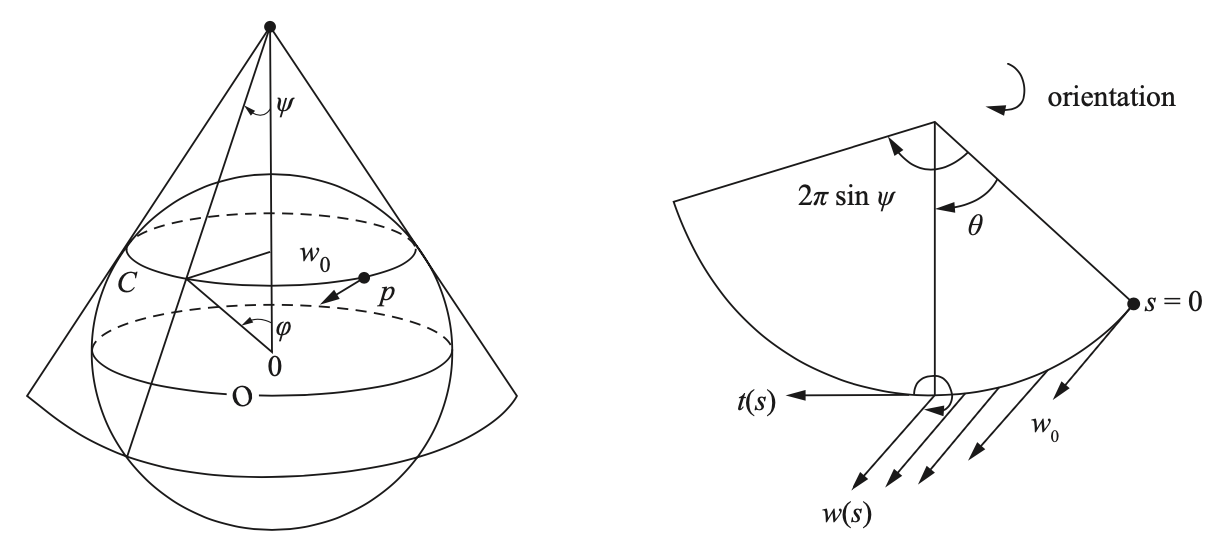
\includegraphics[width=0.7\linewidth]{gauss7}
	\end{figure}
	Aquí observamos que el hecho de que el paralelo $C$ tenga colatitud $\varphi$ implica que el ángulo en el vértice del cono es de $\psi=\pi/2-\varphi$. Luego, pensemos en el cono que es tangente a la esfera a lo largo de $C$ para usar la observación 3 y nuestro trabajo sobre la isometría que conocemos entre el cono menos una generatriz y Pac-Man (Pizza). Recordemos que el ángulo de la Pizza debe ser de $2\pi\sin\varphi$, puesto que es el tamaño de nuestro paralelo (un círculo de radio $\sin\varphi$).
	
	Luego, el transporte paralelo entre dos superficies isométricas es el mismo, ya que la derivada covariante está determinada por los símbolos de Christoffel. Así, un campo paralelo en el cono es enviado a un campo paralelo en la Pizza. ¡Pero la Pizza es plana!
	
	Cuando enviamos el transporte paralelo de $w_0$ a la Pizza, obtenemos un campo paralelo que se ve, como en la figura, como el mismo vector copiado muchas veces a lo largo de la imagen de $C$. Para determinar cómo es el transporte paralelo de $w_0$ en el cono basta decir qué ángulo forma con el vector velocidad de la curva.
	
	Esto es facilísimo de ver en la Pizza: el ángulo es de $2\pi-\theta$, el complemento ángulo del desplazamiento a lo largo de $C$. (Dependiendo de la orientación este ángulo podría ser simplemente $\theta$).
	
	Esto determina completamente al transporte paralelo de $w_0$ porque es el único vector unitario que tiene este ángulo con el vector tangente a la curva. (Aquí usamos que el transporte paralelo es una isometría, pues de esta forma el transporte paralelo de $w_0$ debe ser, en efecto, unitario).
	
	\begin{obs}
		Para que a un desplazamiento de $s$ unidades de tiempo correspona un cambio en el ángulo central de $\theta$, necesitamos la parametrización por longitud de arco. Claro, por esta razón es que se llama "parametrización \textit{por longitud de arco}".
	\end{obs} 
	\vspace{-1cm}
	\begin{figure}[H]
		\begin{subfigure}{0.5\textwidth}
			\centering
			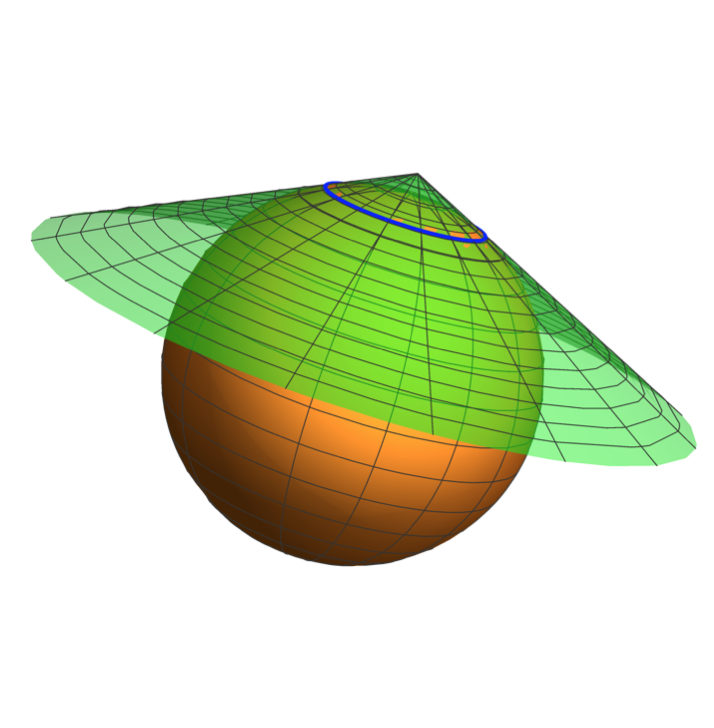
\includegraphics[width=\linewidth]{gauss8}
		\end{subfigure}
		\begin{subfigure}{0.5\textwidth}
			\centering
			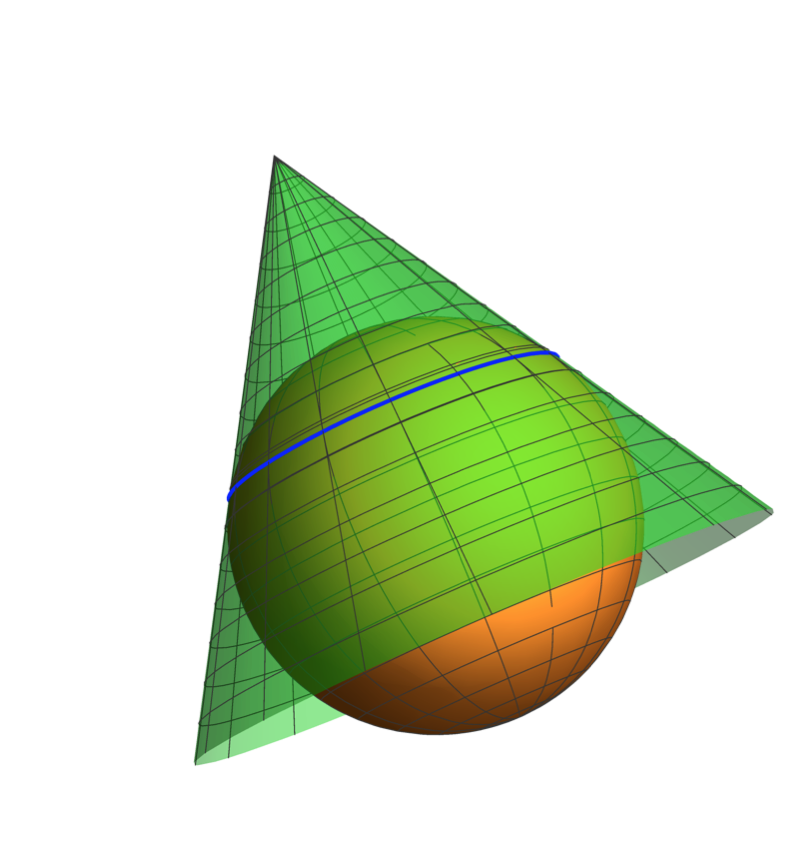
\includegraphics[width=\linewidth]{gauss9}
		\end{subfigure}
	\end{figure}
	\vspace{-3cm}
	\begin{figure}[H]
		\begin{subfigure}{0.5\textwidth}
			\centering
			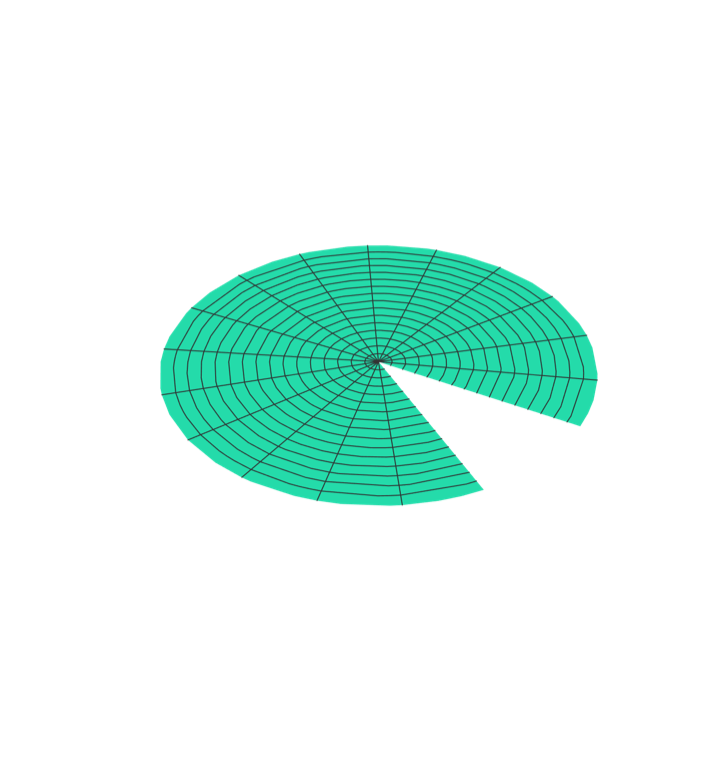
\includegraphics[width=\linewidth]{gauss10}
			\vspace{-2cm}
			\subcaption*{$\varphi=\pi/7$}
		\end{subfigure}
		\begin{subfigure}{0.5\textwidth}
			\centering
			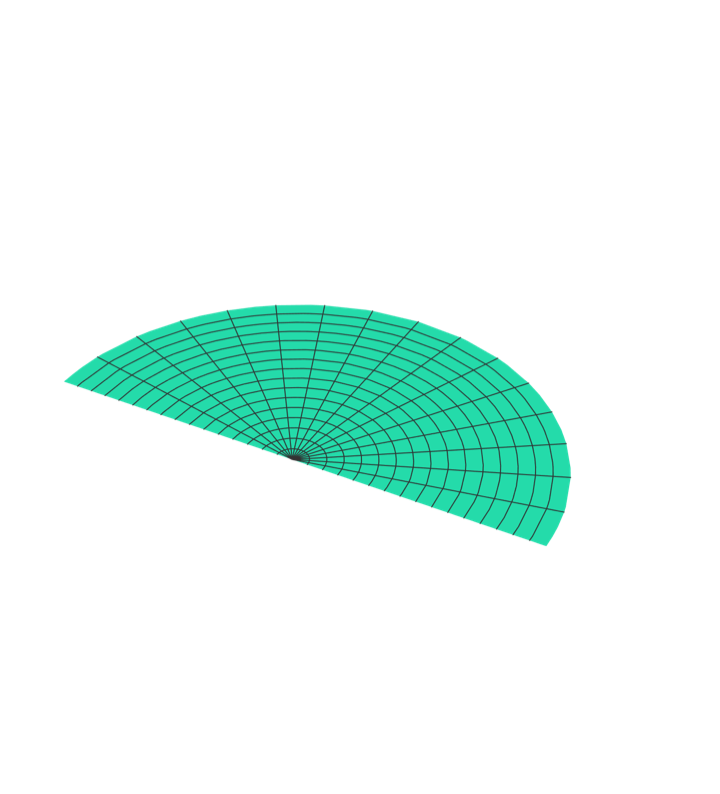
\includegraphics[width=\linewidth]{gauss11}
			\vspace{-2cm}
			\subcaption*{$\varphi=\pi/3$}
		\end{subfigure}
	\end{figure}
\end{ejem}

\section{Geodésicas}
En el ejemplo anterior, el transporte paralelo de un vector tangente a la curva $C$ forma un ángulo de $\theta$ con el vector tangente tras un desplazamiento de ángulo central $\theta$. Esto quiere decir que el transporte paralelo de un vector tangente no coincide con el campo de vectores tangentes a la curva.

En el plano, esto sucede sólo si la curva no es una recta: de otra forma los vectores tangentes forman un campo paralelo, que es constante. Este fenómeno se traduce de igual forma: cuando el campo de vectores velocidad de una curva no es un campo paralelo, la curva se está curvando "más de la cuenta" sobre la superficie. Esto nos lleva a:
\begin{defn}
	Una curva $\alpha:I\to S$ es una \textbf{geodésica}  si $\frac{D\alpha''}{dt}=0$. Es decir, si el campo vectorial de la segunda derivada es paralelo, ie. perpendicular al plano tangente en cada punto.
\end{defn}
\begin{obs}
	Do Carmo define primero "geodésica parametrizada" para el caso de cualquier parametrización de la curva, y luego da otra definición pidiendo la condición sólo para una parametrización por longitud de arco en alguna vecindad local.
\end{obs}
\begin{ejem}
	Toda línea recta contenida en una superficie es una geodésica, pues admite una parametrización por longitud de arco, con la cual tiene segunda derivada igual a cero.
\end{ejem}
\begin{ejem}
	Las geodésicas en la esfera. Consideremos un círculo máximo en $S^2$, que obtenemos al intersectar la esfera con un plano que pasa por el origen. Sabemos que la segunda derivada la parametrización de un círculo tiene la misma dirección que el vector posición (el vector que va del centro del círculo al punto en el círculo). Así, la segunda derivada es de hecho perpendicular al plano tangente.
\end{ejem}
\begin{ejem}
	Las geodésicas en el cilindro. En analogía con la esfera, los círculos paralelos en un cilindro tienen vector normal ortogonal al plano tangente al cilindro, por lo que son geodésicas. Las líneas verticales también. Y, usando que el cilindro es localmente isométrico al plano, la imagen de cualquier recta en el plano bajo esta isometría (que es una hélice) es una geodésica.
\end{ejem}
\begin{figure}[H]
	\centering
	\includegraphics[width=\linewidth]{gauss12}
\end{figure}

\subsection{En coordenadas locales}
Consideremos una curva $\gamma: J\to S$ y un sistema de coordenadas locales $\mathbf x(u,v)$ en alguna vecindad de $\gamma(t_0)$, de forma que curva se expresa como $\gamma(t)=\mathbf x(u(t),v(t))$ y su campo de vectores velocidad $w(t)=u'\mathbf x_u +v'\mathbf x_v$. Recordemos la ecuación $(2)$:
\begin{equation*}
	\begin{aligned}
		\frac{Dw}{dt}&=(a'+\Gamma^1_{11}au'+\Gamma^1_{12}av'+\Gamma^1_{12}bu'+\Gamma^1_{22}bv')\mathbf x_u\\
		&+(b'+\Gamma^2_{11}au'+\Gamma^2_{12}av'+\Gamma^2_{12}bu'+\Gamma^2_{22}bv')\mathbf x_v
	\end{aligned}
\end{equation*}
Sustituyendo con $a=u'$ y $b=v'$,
\begin{equation*}
	\begin{aligned}
		\frac{Dw}{dt}&=(u''+\Gamma^1_{11}(u')^2+2\Gamma^1_{12}u'v'+\Gamma^1_{22}(v')^2)\mathbf x_u\\
		&+(v''+\Gamma^2_{11}(u')^2+2\Gamma^2_{12}u'v'+\Gamma^2_{22}(v')^2)\mathbf x_v
	\end{aligned}
\end{equation*}

Así que para que $\gamma$ sea geodésica simplemente queremos que 
\begin{equation*}
	\begin{aligned}
		u''+\Gamma^1_{11}(u')^2+2\Gamma^1_{12}u'v'+\Gamma^1_{22}(v')^2=0\\
		v''+\Gamma^2_{11}(u')^2+2\Gamma^2_{12}u'v'+\Gamma^2_{22}(v')^2=0
	\end{aligned}
\end{equation*}
Y por teorema de existencia y unicidad, dado un vector tangente en algún punto de una superficie, existe una única geodésica que pasa por el punto en esa dirección.

\subsection{Las geodésicas en una superficie de revolución}
Usaremos las fórmulas que se encontraron para los símbolos de Christoffel de una superficie de revolución parametrizada por
\[\mathbf x(u,v)=(f(v)\cos u,f(v)\sin u,g(v)),\qquad f(v)\neq0\]
Sustituyendo locamente, las ecuaciones diferenciales de las geodésicas se vuelven:
\begin{align*}
	u''+\frac{2ff'}{f^2}u'v'&=0\\
	v''-\frac{ff'}{(f')^2+(g')^2}(u')^2+\frac{f'f''+g'g''}{(f')^2+(g')^2}(v')^2&=0
\end{align*}
Vamos a hacer algunas conclusiones a partir de estas ecuaciones.

Consideremos en primer lugar un meridiano con $u=$ constante, y $v=v(s)$ parametrizado por longitud de arco. La primera ecuación se hace cero y de la segunda quedan dos factores que manejaremos como sigue.

Calculemos el vector tangente al meridiano como función del parámetro $s$:
\[\mathbf x_v(s)= \left(f'(v(s))\cos u,f'(v(s))\sin u,g'(v(s))\right)v'(s)\]
Y de aquí que
\begin{align*}
	G=\langle\mathbf{x}_v(s),\mathbf x_v(s)\rangle= \left(f'(v(s))^2+g'(v(s))^2\right)v'(s)^2\\
	\iff (v')^2=\frac{1}{(f')^2+(g')^2}
\end{align*}
Derivando con cuidado llegamos a que:
\begin{align*}
	2v'v''=\frac{2(f'f''+g'g'')}{\big((f')^2+(g')^2\big)^2}v'=\frac{2(f'f''+g'g'')}{(f')^2+(g')^2}(v')^3\\
	\iff v''=\frac{(f'f''+g'g'')}{(f')^2+(g')^2}(v')^2
\end{align*}
O sea que sí. Ahora veamos qué pasa con $u=u(s)$ y $v=$ constante. La primera ecuación se traduce en que $u'=$ constante y la segunda se vuelve
\[\frac{ff'}{(f')^2+(g')^2}(u')^2=0\]
Ahora $u'\neq0$ para que sí estemos hablando de una curva. Y además, como el denominador es precisamente el valor de $G$, no puede ser cero. Y por fin, $f$ tampoco puede ser cero para que no colapse la superficie. Así es que si nuestra curva es geodésica, $f'=0$, que son los paralelos cuyo radio alcanza un mínimo o un máximo.
\begin{figure}
	\centering
	\includegraphics[width=0.6\linewidth]{gauss13}
\end{figure}
\begin{ejem}[las geodésicas en el paraboloide]
	Las geodésicas en el paraboloide que no son meridianos se intersectan una infinidad de veces. **(Falta)**
\end{ejem}
\begin{prop}[Los caminos más cortos son geodésicas]
	Sea $\alpha: I\to S$ una curva regular con parámetro proporcional a la longitud de arco. Si la longitud de la curva entre cualesquiera dos puntos $t_0$ y $t_1$ en $I$ es menor que la longitud de cualquier curva que pase por $\alpha(t_0)$ y $\alpha(t_1)$ entonces $\alpha$ es una geodésica.
\end{prop}
\begin{obs}
	¿Qué pasa con el recíproco? Necesita ser enunciado en vecindades pequeñas.
\end{obs}
\subsection{Curvatura geodésica}
Definamos un último concepto que será de utilidad en la siguiente sección. Consideremos un campo vectorial diferenciable unitario definido en una curva sobre una superficie. En cada punto de la curva hay una base ortonormal dada por el campo vectorial, el vector normal unitario y el producto cruz de los dos anteriores.

Como el campo vectorial es unitario, $\langle w(t),w(t)\rangle=1$ y derivando obtenemos
\[0=\frac{d}{dt}\langle w(t),w(t)\rangle=2\langle w(t),\frac{d}{dt}w(t)\rangle\]
Así que el campo vectorial es ortogonal a su derivada.

Bueno, el chiste es que entonces la derivada del campo $\frac{d}{dt}w(t)$ está en el plano generado por el vector normal y el producto cruz del normal con el tangente (el tercero de la base que dijimos arriba). Es decir, existen las funciones que hacen cierta esta ecuación:
\[\frac{d}{dt}w(t)=\mu N+\lambda\left(\mathbf N\wedge w(t)\right)\]
Pero además, si consideramos la derivada covariante del campo $\frac{D}{dt}w(t)$, perdemos la componente normal así que simplemente debe existir la función $\lambda$ tal que
\[\frac{D}{dt}w(t)=\lambda\left(\mathbf{N}\wedge w(t)\right)\]
Éste es el \textbf{valor algebraico} de la derivada covariante de $w$ en $t$.

Ahora si pensamos que el campo vectorial es el campo de velocidades de una curva parametrizada por longitud de arco, este valor se llamará la \textbf{curvatura geodésica} y se denotará por $k_g$.

\section{El teorema de Gauss-Bonnet}
Recordemos una de las implicaciones del Teorema de Gauss como la presentó en el abstract de su artículo:
\begin{quotation}
	The excess of the sum of the angles of a triangle formed by shortest lines over two right angles is equal to the total curvature of the triangle.
\end{quotation}
Aunque parece un resultado interesante, de inicio no podemos estar seguros de qué quiere decir porque hace referencia a la "curvatura total" de un triángulo.

Según Do Carmo, esto es lo que quiere decir:
\[\varphi_1+\varphi_2+\varphi_3-\pi=\iint_TKd\sigma\]
donde $\varphi_i$ son los ángulos internos del tríangulo $T$.

La integral es doble porque está definida sobre el dominio de la parametrización, como hacíamos para calcular el área de regiones en superficies. ¿Qué será $d\sigma$? Aunque Do Carmo no lo dice explícitamente, podemos descubrirlo con las siguientes observaciones que hace:
\begin{itemize}
	\item Si la superficie es plana, obtenemos la fórmula conocida de que los ángulos internos de un triángulo suman $\pi$.
	\item Si, por otro lado, la superficie es esférica, la curvatura es constante igual a 1, así que la integral "es exactamente el área de $T$". Para que esto sea cierto necesitamos que el integrando para $K\equiv1$ sea, como sabemos, $\sqrt{EG-F^2}$. Así que de esta forma se define la expresión $d\sigma$, el elemento de área.
	
	Y bueno, como el área de un triángulo es siempre positiva, concluímos que la suma de los ángulos internos de un triángulo esférico es de mayor que $\pi$.
	\item Y bueno, en una superficie como la pseudoesfera con curvatura constante igual a -1, la suma de los ángulos internos es menor que $\pi$.
\end{itemize}
Éste fue el teorema que Gauss demostró en su artículo (con tres consecuencias inmediatas). De acuerdo a Petrunin, Pierre Bonnet y Jacques Binet generalizaron el resultado independientemente para regiones delimitadas por curvas no necesariamente geodésicas.

Tenemos con Do Carmo (sin entrar en detalle de todos los conceptos que aquí se enuncian):
\begin{teo}[Teorema de Gauss-Bonnet local]
	Sea $\mathbf x: U\to S$ una parametrización local ortogonal (para la cual $F=0$) de una superficie orientada $S$. Supongamos que $U$ es homeomorfo a un disco abierto y la parametrización $\mathbf x$ es compatible con la orientación. Sea $R=\mathbf x(U)$ una región simple en la superficie y supongamos que $\alpha:I\to S$ paramaetriza su frontera $\partial R$ con longitud de arco, orientada positivamente y supongamos que $\alpha(s_0),...,\alpha(s_k)$ son los vértices de esta curva y $\theta_0,...,\theta_k$, respectivamente, los ángulos externos en cada vértice.
	Entonces,
	\[\sum_{i=0}^k\int_{s_i}^{s_{i+1}} k_g(s)ds+\iint_R Kd\sigma+\sum_{i=0}^k\theta_i=2\pi\]
	donde $k_g$ es la curvatura geodésica de cada pedazo regular de $\alpha$.
\end{teo}
El siguiente objetivo es dar un resultado que no esté sujeto a una parametrización local. A grandes rasgos, lo que hace Do Carmo es usar varias proposiciones (sin demostrar) para triangular una superficie y usar el resultado local por todos lados.

El concepto de triangulación está íntimamente asociado con un número que se llama \textbf{la característica de Euler}. (Él la llama la característica de Euler-Poincaré, y sí, en efecto aquí Poincaré entra con muchísima potencia por sus ideas relacionadas con la topología, de la cual fue un importante precursor. De hecho algunas de las proposiciones que cita Do Carmo se demuestran en cursos de topología algebraica. Poincaré vivió entre 1854 y 1912, posterior a Riemann).

Bueno, este número tiene una definición muy sencilla:
\[\chi(S)=V-A+C\]
donde $V$ es la cantidad de vértices de la triangulación, $A$ la cantidad de aristas y $C$ la cantidad de caras. Una triangulación es lo que nos imaginamos: una "partición" o teselación de la superficie en triangulitos que cubren toda la superficie y la intersección de sus interiores es vacía.

Los resultados que no podemos demostrar nos aseguran que (1) existen triangulaciones "buenas" para cualquier superficie (lo "bueno" tiene que ver con la orientación de los triángulos), (2) superficies homeomorfas tienen la misma característica de Euler, (3) las únicas superficies compactas y conexas en $\R^3$ son homeomorfas a sumas conexas de toros o a la esfera, y (4) se pueden integrar funciones en superficies usando triangulaciones bastante finas como para que cada triángulo esté contenido en una parametrización local y de hecho la integral no depende ni de la triangulación ni de las parametrizaciones.

Bueno, el chiste es que con todo esto Do Carmo muestra que:
\begin{teo}[Teorema de Gauss-Bonnet global]
	Sea $R\subseteq S$ una región regular de una superficie orientada $S$. Sean $C_1,...,C_n$ las curvas cerradas simples y regulares por pedazos que conforman la frontera de $R$. Supongamos que cada una de las $C_i$ tiene una orientación positiva, de tal forma que podemos definir sus ángulos externos $\theta_1,...,\theta_p$. Entonces
	\[\sum_{i=0}^k\int_{C_i} k_g(s)ds+\iint_R Kd\sigma+\sum_{i=0}^p\theta_i=2\pi\chi(R)\]
	donde $s$ es una parametrización por longitud de arco de cada $C_i$ y la integral sobre $C_i$ está definida como la suma de las integrales en cada pedazo regular.
\end{teo}
Y bueno, todo esto para decir que para una superficie compacta orientable $S$,
\[\iint_SKd\sigma=2\pi\chi(S)\]
ya que no tiene frontera.

\subsection{Implicaciones}
Ahora veamos algunas implicaciones de este brutal resultado.
\begin{prop}
	Toda superficie compacta con curvatura positiva es homeomorfa a una esfera.
\end{prop}
\begin{proof}
Como dijimos (sin demostrar) las únicas superficies compactas  en $\R^3$ son homeomorfas a la esfera o sumas conexas de toros.
\begin{itemize}
	\item La esfera tiene característica de Euler 2, lo que se puede corroborar haciendo la cuenta para cualquier sólido platónico (el caso más fácil es el tetraedro).
	\item Para calcular la característica de Euler del todo usaremos los diagramas de Hatcher, Algebraic Topology. Aquí usamos \textbf{descomposiciones CW} para las superficies, que son como triangulaciones, pero más fáciles de manejar.
	
	El toro tiene característica de Euler 0, como podemos ver en este dibujo:
	\begin{figure}[H]
		\centering
		\includegraphics[width=0.7\linewidth]{gauss14}
	\end{figure}
	\item La superficie de género $g$, denotada por $S_g$ (si el toro tiene 1 hoyo, ésta tiene $g$ hoyos) tiene característica de Euler
	\[\chi(S)=2g-2\]
	\begin{itemize}
		\item Veamos el caso para $g=2$ en analogía con el ejemplo anterior:
		\begin{figure}[H]
			\centering
			\includegraphics[width=0.7\linewidth]{gauss15}
		\end{figure}
		\item Y de una vez mostrmos $g=3$ aprovechando los diagramas de Hatcher
		\begin{figure}[H]
			\centering
			\includegraphics[width=0.7\linewidth]{gauss16}
		\end{figure}
		O sea que la característica de Euler para superficies compactas en $\R^3$ puede ser $2, 0, -2, -4, -6, \ldots$
		\vspace{-.5cm}
	\end{itemize}
\end{itemize}
\end{proof}
Como segunda implicación, estudiemos los ángulos de un triángulo geodésico. Comenzamos enunciando el teorema de Gauss-Bonnet como lo enunció Gauss en su artículo Disquisitiones Circa Superficies Curvas. Comentamos que la suma de los ángulos internos de un triángulo geodésico es:
\begin{itemize}
	\item Igual a $\pi$ para superficies con $K\equiv0$.
	\item Mayor que $\pi$ para superficies con curvatura positiva.
	\item Menor que $\pi$ para superficies con curvatura negativa.
\end{itemize}
De hecho, el resultado para curvatura nula es equivalente al quinto postulado de Euclides. Así que las superficies con curvatura positiva o negativa están a nada de ser modelos de geometría no euclidiana. Pero, ¿qué falta? El axioma 2 de Euclides: cualquier línea (para nosotros, geodésica) puede ser extendida indefinidamente. Chin, parece que en las superficies que conocemos con curvatura constante diferente de cero siempre hay geodésicas cerradas (¿qué pasa con la pseudoesfera?).
\begin{figure}
	\centering
	\includegraphics[width=0.7\linewidth]{gauss17}
\end{figure}
Y de hecho, en 1901 Hilbert demostró que no existe una superficie regular en $\R^3$ con curvatura constante negativa cuyas geodésicas se puedan extender indefinidamente, mostrando así que la geometría no euclidiana (hiperbólica) no se puede modelar globalmente por una superficie regular en $\R^3$.

Mostramos el teorema en la versión que prueba Do Carmo hacia el final de su libro (usando ideas que no hemos definido, sobre todo el de superficie abstracta y encaje):
\begin{teo}[Hilbert]
	Una superficie geométrica completa (sus geodésicas se pueden extender indefinidamente) con curvatura constante negativa no se puede encajar isométricamente en $\R^3$.
\end{teo}
Y hay muchas otras implicaciones y generalizaciones de este teorema.
\begin{ejer}[Círculos en una superficie con $K>1$. Petrunin, What is differential geometry? Ejer 15.2]
	Terminaremos estas notas considerando una curva regular $\gamma:I\to S$ cerrada y sin intersecciones en una superficie $S$ con curvatura Gaussiana positiva. Mostraremos que si la curvatura geodésica de $\gamma$ es constante igual a 1, entonces su longitud es menor que $2\pi$.
	
	Para dar un significado geométrico a este problema notemos que una curva plana con curvatura geodésica constante igual a 1 es un círculo. Claro, al inicio del curso dijimos que dada la función de curvatura de una curva plana existe una única curva salvo movimientos rígidos en el plano (traslaciones, rotaciones y reflexiones) que tiene esa curvatura.
\end{ejer}
\begin{proof}[Solución]
	Pensando que esta curva es la frontera de un disco topológico $\Delta$ en la superficie (por ahora supongámoslo), podemos aplicar Gauss-Bonnet. Como la curva es regular, los ángulos $\theta_i$ son cero, así que obtenemos
	\[\int_{s_0}^{s_1} k_g(s)ds+\iint_\Delta Kd\sigma=2\pi\]
	Pero si la curvatura geodésica es 1, entonces la integral es la longitud de $\gamma$, y como la curvatura es positiva, terminamos.
	
	Para ver que esta curva es la frontera de un disco, deberíamos argumentar que (1) la superficie se puede parametrizar con una función diferenciable y regular $\mathbf x:S^1\to S$ (la superficie es "una esfera suave") y (2) una curva cerrada simple en una esfera suave divide la superficie en dos discos topológicos (teorema de Jordan).
	
	Esto es, "los círculos" en una superficie con curvatura positiva miden menos que $2\pi$.\nocite{DoCarmo}
\end{proof}
\chapter{Referencias}
\printbibliography
\end{document}